\documentclass[10pt,twocolumn,a4paper]{article}

% ---- Packages ----
\usepackage[utf8]{inputenc}
\usepackage[T1]{fontenc}
\usepackage{lmodern}              % Computer Modern (IEEE-trans uses Times; lmodern is the widely-available alternative)
\usepackage[top=1.8cm,bottom=1.8cm,left=1.6cm,right=1.6cm]{geometry}
\usepackage{microtype}
\usepackage{amsmath}
\usepackage{amssymb}
\usepackage{booktabs}
\usepackage{enumitem}
\usepackage{titlesec}
\usepackage{xcolor}
\usepackage{hyperref}
\usepackage{tabularx}
\usepackage{array}
\usepackage{colortbl}
\usepackage{graphicx}
\usepackage{fancyhdr}
\usepackage[numbers,sort&compress]{natbib}
\usepackage{url}
\usepackage{caption}
\usepackage{subcaption}
\usepackage{tikz}
\usepackage{calc}
\usepackage{needspace}
\usepackage{listings}
\usepackage{float}
\usetikzlibrary{positioning,calc,patterns,shapes.geometric}

% IEEE-trans-like column geometry: 0.6 cm column separation
\setlength{\columnsep}{0.55cm}

% ---- Colors (Maastricht University palette, retained as institutional accent) ----
\definecolor{umdark}{HTML}{001C3D}
\definecolor{umorange}{HTML}{E84E10}
\definecolor{umlight}{HTML}{4A90C4}
\definecolor{umgray}{HTML}{6B7280}
\definecolor{codebg}{HTML}{F6F8FA}
\definecolor{codekw}{HTML}{0550AE}
\definecolor{codestr}{HTML}{0A6D38}
\definecolor{codecmt}{HTML}{6B7280}

% ---- Formatting ----
\hypersetup{colorlinks=true,linkcolor=umdark,citecolor=umlight,urlcolor=umlight}
\setlength{\parskip}{1pt plus 0.5pt}
\setlength{\parindent}{1em}

% IEEE-trans-style section headings: numbered Roman, small caps, no rule.
\renewcommand{\thesection}{\Roman{section}}
\renewcommand{\thesubsection}{\Alph{subsection}}
\renewcommand{\thesubsubsection}{\arabic{subsubsection})}
\titleformat{\section}[block]{\normalfont\centering\bfseries\small\scshape}{\thesection.}{0.5em}{}
\titleformat{\subsection}[block]{\normalfont\bfseries\small\itshape}{\thesubsection.}{0.5em}{}
\titleformat{\subsubsection}[runin]{\normalfont\itshape\small}{\thesubsubsection}{0.4em}{}[:\hspace{0.3em}]
\titlespacing*{\section}{0pt}{12pt plus 2pt}{4pt plus 1pt}
\titlespacing*{\subsection}{0pt}{8pt plus 2pt}{2pt plus 1pt}
\titlespacing*{\subsubsection}{0pt}{4pt plus 1pt}{0pt}

\setlist{topsep=2pt,itemsep=1pt,parsep=0pt,leftmargin=1.4em}

% IEEE-trans caption style: bold "Fig. N." / "TABLE N." labels, footnotesize body, justified.
\captionsetup{font=footnotesize,labelfont={footnotesize,bf},labelsep=period,skip=3pt,justification=raggedright,singlelinecheck=false}
\captionsetup[figure]{name=Fig.}
\captionsetup[table]{name=TABLE,position=top,font={footnotesize,sc},labelfont={footnotesize,sc},labelsep=newline,justification=centering,singlelinecheck=true}
\captionsetup[subfigure]{font=scriptsize,labelfont={scriptsize,bf}}

% Code listings: thin frame, no background, IEEE-style numbered listing.
\lstdefinestyle{pystyle}{
  language=Python,
  basicstyle=\ttfamily\scriptsize,
  keywordstyle=\color{codekw}\bfseries,
  stringstyle=\color{codestr},
  commentstyle=\color{codecmt}\itshape,
  numbers=left,
  numberstyle=\tiny\color{codecmt},
  numbersep=4pt,
  frame=tb,
  framerule=0.5pt,
  framesep=2pt,
  xleftmargin=4pt,
  xrightmargin=0pt,
  breaklines=true,
  showstringspaces=false,
  columns=fullflexible,
  keepspaces=true,
  belowskip=3pt,
  aboveskip=4pt,
}
\lstset{style=pystyle}

\pagestyle{fancy}
\fancyhf{}
\renewcommand{\headrulewidth}{0pt}
\fancyfoot[C]{\small\thepage}

% ============================================================
% Title
% ============================================================
\title{\vspace{-1.4cm}\textbf{Does the Source of the Carrier Image Affect\\
Steganographic Detectability?}}
\author{\normalsize
Abdul~Moiz~Akbar,\quad
Daria~Gjonbalaj,\quad
Nico~M\"uller-Sp\"ath,\quad
Jimena~Narvaez~del~Cid,\quad
David~Wicker,\quad
Nikolas~Zouros\\[2pt]
\small \textit{Department of Advanced Computing Sciences, Maastricht University},\enskip May 2026}
\date{}

\begin{document}
\twocolumn[
\begin{@twocolumnfalse}
\maketitle
\thispagestyle{fancy}
\vspace{-0.8cm}
\begin{center}
\begin{minipage}{0.86\textwidth}\small
\noindent\textbf{Abstract}---We ask whether the source of a carrier image, a real photograph or an AI-generated one, changes how detectable LSB steganography is under fixed embedding settings. On a corpus of 3{,}000 caption-matched image groups spanning three carrier sources (real, SDXL, FLUX.1-schnell), two embedding branches (spatial LSB on PNG, JSteg-style DCT-LSB on JPEG~Q=95), three payload levels, and plain vs.\ AES-256-CBC payloads, we evaluate six training-free detectors under a pre-registered DeLong $+$ Bonferroni--Holm protocol. The carrier-source effect is small and payload-dependent (pooled $|\Delta_\text{AUC}|\!\approx\!0.013$, mostly below the pre-registered $0.05$ practical-significance threshold), but consistently signed toward AI carriers being easier to attack in five of six detectors; the sixth ($\chi^2$-spatial) reverses on full AUC, though the reversal dissolves at operational false-positive rates. Restricting the ROC to FPR\,$\leq\!0.10$ amplifies the effect $3$ to $7\times$ and renders it consistently significant. Cross-validating on two learned detectors (SRNet, DCTR with an LDA ensemble) trained on a separate matched corpus reproduces the classical pattern. A real-only-training ablation then reveals that SRNet's apparent source-invariance is an artefact of balanced training: withholding AI carriers opens a per-source gap of up to $0.44$~AUC on AI test images (partly confounded by training-corpus composition at the smaller end). Two further contributions: a tile-local Westfeld~$\chi^2$ variant validated on BOSSBase~1.01 ($+0.09$~AUC over the global test on JSteg at both Q$=$75 and Q$=$95), and a candidate variance-inflation mechanism for the $\chi^2$-spatial reversal.

\smallskip
\noindent\textit{\textbf{Index Terms}---steganography, steganalysis, LSB embedding, cover-source mismatch, diffusion models, paired DeLong test, partial AUC.}
\end{minipage}
\end{center}
\vspace{0.4cm}
\end{@twocolumnfalse}
]

% ============================================================
\section{Introduction}
\label{sec:intro}
% ============================================================

Steganography is the practice of concealing the existence of a message inside an innocuous host medium, typically a digital image~\cite{petitcolas1999,cheddad2010}. Its complement, steganalysis, is the detection problem an adversary faces: given a file, decide whether it carries a hidden payload. Because every embedding rule must perturb the cover, every detector exploits the same residual signal, a statistical irregularity introduced into pixel intensities or frequency coefficients~\cite{westfeld1999chi,fridrich2001lsb,dumitrescu2003sp}. The size and shape of that irregularity, however, depend not only on the embedding rule but also on the cover itself, an issue formalised as cover-source mismatch~\cite{giboulot2020csm,mallet2024csm}.

For two decades, the published benchmarks have implicitly assumed the cover is a photograph carrying the noise pattern and JPEG history of a real camera pipeline. Latent-diffusion models such as Stable Diffusion XL~\cite{sdxl2023} and FLUX.1~\cite{flux2024} now produce photorealistic images at scale through a process that contains none of the sensor noise, demosaicing, or in-camera JPEG steps a detector would expect. Corvi~\textit{et~al.}~\cite{corvi2023diffusion} reported that diffusion outputs leave their own characteristic spectral fingerprints, and a small recent literature on cover-source mismatch for synthetic carriers~\cite{mereur2024deepfake,mallet2024csm} has begun to ask whether classical steganalysis still works when the cover is generated rather than captured. The literature so far has not, however, looked at this at the level of detector-pair contrasts on a controlled, caption-matched dataset.

This article addresses that gap. We build a corpus of $N\!=\!3{,}000$ caption-matched image groups across three carrier sources, two embedding branches, three payload levels, and two payload conditions (plain and AES-256-CBC), evaluate six training-free statistical detectors under a pre-registered DeLong + Bonferroni--Holm protocol, and cross-validate every pre-registered finding on a fundamentally different class of detectors (the deep residual network SRNet~\cite{boroumand2019srnet} and the undecimated-DCT feature set DCTR~\cite{holub2015dctr} with an LDA ensemble~\cite{fridrich2012srm}). Two further contributions arise from the analysis of individual detectors that under- or out-perform the field.

\paragraph{Contributions.} This work makes four contributions:
\begin{enumerate}
\item A corpus of 3{,}000 caption-matched image groups and a pre-registered, training-free six-detector evaluation of the carrier-source effect (real vs.\ diffusion generated) on LSB-style steganography, with paired DeLong tests, Bonferroni--Holm correction, and a partial-AUC analysis at FPR\,$\leq\!0.10$ (Sections~\ref{sec:methods}, \ref{sec:results-classical}).
\item A cross-validation of every pre-registered finding on a fundamentally different class of learned detectors (SRNet, DCTR) trained on a separate, matched dataset, in two complementary configurations, \textit{matched training} (1:1:1 real/SDXL/FLUX) and \textit{real-only training} (AI carriers held out). The matched-vs-real-only \emph{contrast} shows that SRNet's apparent source-invariance under matched training comes from the balanced training mix rather than anything architectural: removing AI carriers from training opens a $0.26$--$0.45$~AUC gap on AI test carriers (with a partially-confounded smaller end, see Section~\ref{sec:limitations}; Section~\ref{sec:learnedxval}).
\item A tile-local variant of the Westfeld pairs-of-values $\chi^2$ test for the DCT domain that out-performs its global counterpart by a large margin in the spatial-heterogeneity regime characteristic of diffusion carriers, accompanied by a set of recommended validation experiments to establish its generality beyond the present corpus (Section~\ref{sec:tiled}).
A candidate mechanism for the $\chi^2$-spatial reversal, the single detector that reports the opposite carrier-source ordering from its peers (an effect that is operationally negligible: it dissolves under partial AUC at FPR\,$\leq\!0.10$). The naive ``smoother diffusion outputs'' hypothesis is falsified directly on cover-side pair-of-values imbalance; a correlational variance-inflation argument is offered in its place (Section~\ref{sec:chi2spatial}).
\end{enumerate}

\paragraph{Paper organisation.} Section~\ref{sec:relatedwork} reviews relevant prior work. Section~\ref{sec:methods} describes the dataset, embedding pipeline, detector suite, and statistical protocol. Section~\ref{sec:experiments} reports the experimental configuration. Section~\ref{sec:results-classical} presents the pre-registered classical-detector results across the five research questions. Section~\ref{sec:learnedxval} reports the learned-detector cross-validation and the real-only-training ablation. Section~\ref{sec:detector-side} develops the two detector-side findings: the tile-local $\chi^2$-DCT proposal with its recommended validation experiments, and the $\chi^2$-spatial reversal analysis. Section~\ref{sec:discussion} integrates the four contributions; Sections~\ref{sec:limitations} and \ref{sec:conclusion} cover limitations and conclusions.

% ============================================================
\section{Related Work}
\label{sec:relatedwork}
% ============================================================

\subsection{Classical LSB Embedding and Detection}
The simplest spatial-domain stego method, \textbf{LSB replacement}, overwrites the least-significant bit of each pixel with payload bits~\cite{petitcolas1999,hussain2018}. In JPEG carriers, the analogous JSteg variant overwrites the LSBs of non-zero quantised AC DCT coefficients~\cite{westfeld1999chi,fridrich2003calib}. Both leave detectable traces.

The \textbf{Westfeld $\chi^2$ attack}~\cite{westfeld1999chi} tests whether adjacent value pairs $\{2k,2k\!+\!1\}$ have moved toward equal frequency, the diagnostic signature of LSB replacement. \textbf{RS Analysis}~\cite{fridrich2001lsb} tracks changes in Regular and Singular pixel-group counts under flipping masks. \textbf{Sample Pairs analysis} (SPA)~\cite{dumitrescu2003sp} estimates the embedded fraction from trace multisets on adjacent pixel pairs. In the frequency domain, Fridrich~et~al.'s \textbf{calibration $\chi^2$}~\cite{fridrich2003calib} introduced a non-block-aligned crop-recompress reference that approximates a payload-free histogram. All five are training-free and have closed-form scores; this makes them attractive for a comparison study because any AUC difference between carrier groups cannot be attributed to training-set bias.

\subsection{AI-Generated Carriers}
Gao~et~al.~\cite{gao2022ai} use generative models to encode steganographic secrets as the generated image itself (coverless steganography). That setting differs from ours, where a payload is embedded \emph{into} an existing cover. The closest prior work is M\'{e}reur~et~al.~\cite{mereur2024deepfake}, who test 15 GAN- and diffusion-based image generators as carriers under three adaptive spatial embeddings (HILL, S-UNIWARD, MiPOD) at 0.4~bpp, against an SRMQ1 + low-complexity linear classifier and an EfficientNet-v2 deep classifier, and report classifier-error rate $P_E$. The two studies are complementary rather than directly comparable: M\'ereur+24 probes high-payload adaptive embeddings against learned detectors on unpaired generator pools, while we probe low-payload non-adaptive embeddings against training-free detectors on a caption-matched factorial. Mallet~et~al.~\cite{mallet2024csm} provide a systematic survey of cover-source mismatch and document that classical detectors built on one cover distribution often degrade on another. Table~\ref{tab:relatedwork} contrasts our design against the closest prior work along five axes that matter for cross-comparison.

\begin{table*}[t]
\centering\footnotesize
\caption{Closest prior work vs.\ this study. ``Match'' is the caption-matched-across-carriers design; no prior reference combines all five axes.}
\label{tab:relatedwork}
\setlength{\tabcolsep}{4pt}\renewcommand{\arraystretch}{1.15}
\begin{tabular}{@{}l c c c c c@{}}
\toprule
\textbf{Reference} & \textbf{Carrier} & \textbf{Embedding} & \textbf{Detector} & \textbf{Metric} & \textbf{Match} \\
\midrule
Westfeld+99~\cite{westfeld1999chi}      & photo            & LSB / JSteg     & $\chi^2$ PoV          & p-value    & --- \\
Fridrich+01~\cite{fridrich2001lsb}      & photo            & LSB             & RS                    & est.\ embedding rate & --- \\
Dumitrescu+03~\cite{dumitrescu2003sp}   & photo            & LSB             & SPA                   & est.\ embedding rate & --- \\
Fridrich+03~\cite{fridrich2003calib}    & photo (JPEG)     & JSteg           & calibration $\chi^2$  & distance   & --- \\
SRM+12~\cite{fridrich2012srm}           & photo (BOSS)     & HUGO/HILL       & ensemble (learned)    & $P_E$      & --- \\
SRNet+19~\cite{boroumand2019srnet}      & photo (BOSS)     & adaptive        & deep CNN              & $P_E$      & --- \\
Gao+22~\cite{gao2022ai}                 & GAN-coverless    & secret-sharing  & ---                   & ---        & --- \\
Corvi+23~\cite{corvi2023diffusion}      & diffusion        & none (detection only) & CNN forensics   & AUC        & no  \\
M\'ereur+24~\cite{mereur2024deepfake}   & real + 15 gen.   & HILL / S-UNIW / MiPOD  & SRMQ1+LC / EffNet-v2  & $P_E$      & no  \\
\midrule
\textbf{This work} & \textbf{real + 2 diffusion} & \textbf{LSB / DCT-LSB} & \textbf{6 training-free} & \textbf{paired AUC + pAUC} & \textbf{yes} \\
\bottomrule
\end{tabular}
\end{table*}

\subsection{Cover-Source Mismatch and the Role of Learned Detectors}
Cross-domain steganalysis was first formalised for camera-to-camera shifts: Giboulot~et~al.~\cite{giboulot2020csm} and Mallet~et~al.~\cite{mallet2024csm} show detectors trained on one cover source degrade on another. Our setting extends this to a larger shift, from natural photographs to latent-diffusion outputs, which Corvi~et~al.~\cite{corvi2023diffusion} demonstrate carry distinct low-frequency fingerprints. Trained detectors, SRNet~\cite{boroumand2019srnet}, DCTR~\cite{holub2015dctr}, SRM~\cite{fridrich2012srm}, typically outperform training-free baselines on within-distribution benchmarks, but any AUC gap between carrier groups under a learned detector could be a training-set artefact rather than a carrier-statistics property. We therefore use training-free detectors for the \emph{primary} analysis (unambiguous causal attribution) and add a learned-detector \emph{cross-validation} (SRNet + DCTR), trained on a separate caption-matched dataset disjoint from the test set by caption~ID, not on BOSSBase~\cite{bas2011boss}, in two configurations: \emph{matched training} (all carrier sources present) and \emph{real-only training} (AI carriers held out, isolating whether SRNet's apparent source-invariance is architectural or a training-balance artefact; Section~\ref{sec:v2a}).

% ============================================================
\section{Methodology}
\label{sec:methods}
% ============================================================

\subsection{Research Questions and Pre-Registration}
The five research questions were fixed in the project proposal, with $\delta_\text{min}\!=\!0.05$ as the pre-registered practical-significance threshold:
\begin{description}[font=\bfseries,leftmargin=1.2em,style=nextline,itemsep=2pt]
\item[RQ1 (primary, confirmatory)] Does carrier source (real vs.\ pooled AI) affect detectability under matched embedding?
\item[RQ2 (primary, confirmatory)] Within AI carriers, does the generator (SDXL vs.\ FLUX.1-schnell) change detectability?
\item[RQ3 (exploratory)] Does payload size modulate the source effect?
\item[RQ4 (exploratory)] Do the spatial (LSB+PNG) and frequency (DCT-LSB+JPEG) branches show different source effects?
\item[RQ5 (verification)] Does AES-256-CBC encryption of the payload affect detectability? Expected null.
\end{description}

\subsection{Dataset Construction}
\label{sec:dataset}
The \textbf{caption-matched design} holds the semantic prompt fixed across sources, reducing (though not eliminating) subject-matter confounding: a real photograph and a generated image conditioned on the same caption can still differ in layout, object count, texture density, and photographic statistics, so caption matching minimises rather than removes semantic shift. For each of $N\!=\!3{,}000$ groups we draw one caption from COCO~\cite{coco2014} or Flickr30k~\cite{flickr30k2014} and produce three covers: a \textbf{real} photograph (the original source image, distributed as JPEG), an \textbf{AI-A} image from SDXL~1.0~\cite{sdxl2023}, and an \textbf{AI-B} image from FLUX.1-schnell~\cite{flux2024} (both pristine PIL outputs). All three are converted to 8-bit grayscale ($0.299R\!+\!0.587G\!+\!0.114B$), centre-resized to $512\!\times\!512$, and stored both as lossless PNG (spatial branch input) and as JPEG~Q=95 (frequency branch input). A consequence of the source-format asymmetry: the frequency-branch real covers carry a double-compression history (original JPEG $\to$ decode $\to$ Q=95 re-encode), while the AI covers carry a single Q=95 compression. The spatial branch is unaffected (lossless PNG storage); the frequency-branch implication is discussed as a confound in Section~\ref{sec:limitations}.

The change of the AI-B model from the proposal's PixArt-$\alpha$~\cite{pixart2023} to FLUX.1-schnell was forced by HF Inference API availability; both are transformer-based diffusion models sharing the conceptual role in the comparison. Per group the pipeline produces 3 logical covers and 12 stego variants per source (2 methods $\times$ 3 payloads $\times$ 2 encryption conditions): 39 logical images per group and 117{,}000 across the full run (Figure~\ref{fig:factorial}). Because each logical cover is stored in both branch formats (PNG, JPEG) while each stego file is branch-specific, the on-disk artefact count is 18{,}000 cover files ($9{,}000\!\times\!2$) plus 108{,}000 stego files ($9{,}000\!\times\!12$).

\begin{figure}[t]
\centering
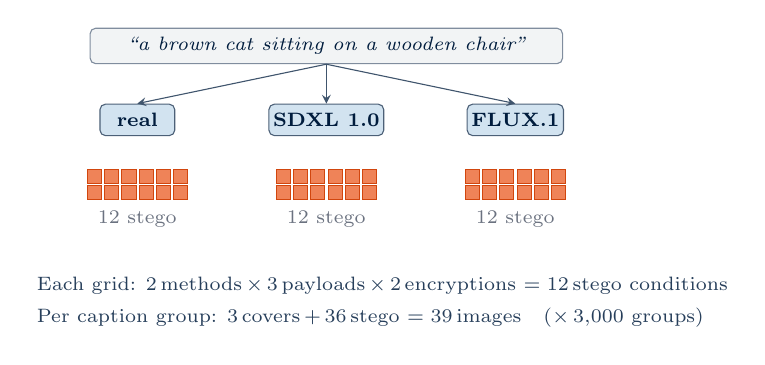
\begin{tikzpicture}[
  capbox/.style={draw=umdark!50, fill=umdark!5, rounded corners=2pt, font=\scriptsize\itshape\color{umdark}, inner sep=2pt, minimum width=6.0cm, minimum height=0.45cm, align=center},
  srcbox/.style={draw=umdark!70, fill=umlight!25, rounded corners=2pt, font=\scriptsize\bfseries\color{umdark}, inner sep=1.5pt, minimum width=0.95cm, minimum height=0.4cm, align=center},
  condcell/.style={draw=umorange!90!black, fill=umorange!70, inner sep=0pt, minimum width=0.18cm, minimum height=0.18cm, line width=0.2pt},
  parrow/.style={->, >=stealth, umdark!75, line width=0.4pt},
]
% Caption at top
\node[capbox] (cap) {``a brown cat sitting on a wooden chair''};

% Three source nodes
\node[srcbox, below=0.50cm of cap, xshift=-2.4cm] (real) {real};
\node[srcbox, below=0.50cm of cap]                (mla)  {SDXL 1.0};
\node[srcbox, below=0.50cm of cap, xshift= 2.4cm] (mlb)  {FLUX.1};

% Arrows from caption
\draw[parrow] (cap.south) -- (real.north);
\draw[parrow] (cap.south) -- (mla.north);
\draw[parrow] (cap.south) -- (mlb.north);

% 12-condition grid under each source: 2 rows x 6 cols
\foreach \xc/\src in {-2.4/real, 0/mla, 2.4/mlb} {
  \foreach \r in {0,1} {
    \foreach \c in {0,1,2,3,4,5} {
      \pgfmathsetmacro{\xx}{\xc - 0.55 + 0.22*\c}
      \pgfmathsetmacro{\yy}{-1.65 - 0.21*\r}
      \node[condcell] at (\xx,\yy) {};
    }
  }
}
% Labels below conditions
\node[font=\scriptsize\color{umgray}] at (-2.4,-2.20) {12 stego};
\node[font=\scriptsize\color{umgray}] at ( 0  ,-2.20) {12 stego};
\node[font=\scriptsize\color{umgray}] at ( 2.4,-2.20) {12 stego};

% Legend explaining grid
\node[font=\scriptsize\color{umdark!85}, align=left, anchor=west] at (-3.8,-3.05) {Each grid: $2$\,methods\,$\times\,3$\,payloads\,$\times\,2$\,encryptions $=12$\,stego conditions};
\node[font=\scriptsize\color{umdark!85}, align=left, anchor=west] at (-3.8,-3.45) {Per caption group: $3$\,covers\,+\,$36$\,stego $=39$\,images\quad($\times\,3{,}000$ groups)};
\end{tikzpicture}
\caption{Caption-matched study design ($3$ sources $\times\,2$ methods $\times\,3$ payloads $\times\,2$ encryptions). Each of $N\!=\!3{,}000$ caption groups produces three covers (one per carrier source) under the same caption, then a per-source $2$-method $\times\,3$-payload $\times\,2$-encryption grid of stego variants. Caption matching constrains the semantic prompt across sources to minimise subject-matter confounding; residual layout/object-count/texture differences remain.}
\label{fig:factorial}
\end{figure}

\subsection{Embedding Pipeline}
\label{sec:embedding}

\paragraph{Spatial branch (LSB substitution).} Replace the least-significant bit of each pixel in row-major order with payload bits, $k\!=\!1$, until the target fill fraction is reached. Storage is lossless PNG. The mechanism is illustrated in Figure~\ref{fig:lsbdct}~(left).

\paragraph{Frequency branch (JSteg-style DCT-LSB).} Flip the LSB of each non-zero quantised AC DCT coefficient in row-major block order. We skip DC and $|c|\!=\!1$ coefficients to avoid the Westfeld-pair instability they create. Re-entropy-coding uses the same Q=95 table without re-quantisation. The mechanism is illustrated in Figure~\ref{fig:lsbdct}~(right).

\paragraph{Payload levels.} The proposal's original fill rates of $\{0.25,\,0.50,\,0.75\}$ caused near-saturation on the strongest detectors (AUC$\,>\,0.99$), erasing the carrier-source signal. We revised them to $\{0.05,\,0.15,\,0.30\}$~bpp, which is also closer to operationally realistic embedding rates. Both branches use $k\!=\!1$ throughout.

\paragraph{Encryption.} Payloads are tested in two conditions, \emph{plain} (raw bitstream) and \emph{AES-256-CBC} (random IV per message; key fixed per run), in both branches. The encrypted condition tests whether detectors are reacting to plaintext structure rather than to embedding distortion.

\paragraph{Payload distribution.} \emph{Plain} is a uniform random bytestream produced by a seeded RNG, not human-readable text, the standard steganalysis-benchmark choice~\cite{boroumand2019srnet,holub2015dctr} reflecting a threat model where any sophisticated attacker encrypts before embedding. Both \emph{plain} and \emph{AES-256-CBC} therefore produce maximum-entropy payloads; RQ5 empirically validates this assumption.

\begin{figure*}[t]
\centering
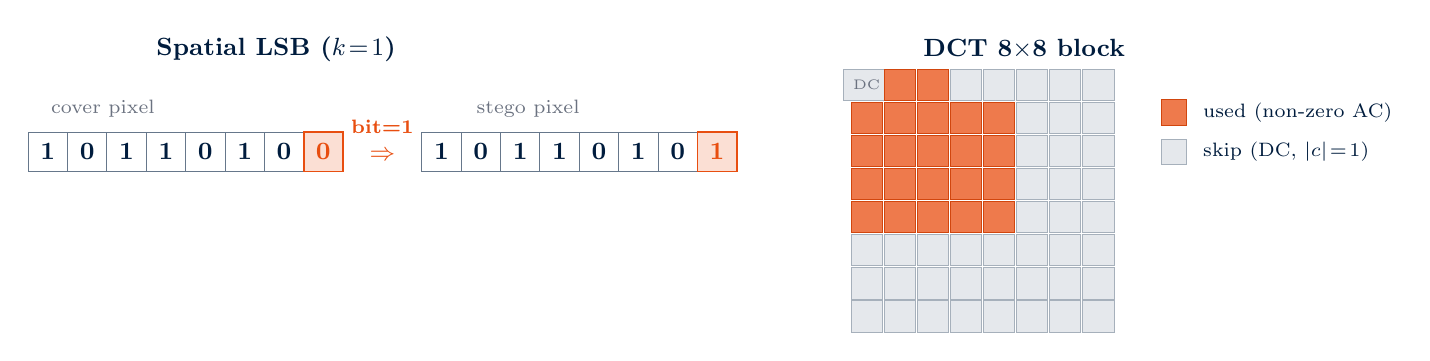
\begin{tikzpicture}[node distance=0.4cm,
  bitcell/.style={draw=umdark!60, minimum width=0.50cm, minimum height=0.50cm, font=\small\bfseries\color{umdark}, line width=0.3pt},
  bitlsb/.style={draw=umorange, fill=umorange!18, minimum width=0.50cm, minimum height=0.50cm, font=\small\bfseries\color{umorange}, line width=0.6pt},
  dctused/.style={draw=umorange!90!black, fill=umorange!75, minimum width=0.40cm, minimum height=0.40cm, line width=0.3pt},
  dctskip/.style={draw=umdark!35, fill=umdark!10, minimum width=0.40cm, minimum height=0.40cm, line width=0.3pt, font=\tiny\color{umgray}},
]
% Left panel: LSB illustration. Origin near x=-7.
\node[font=\small\bfseries\color{umdark}] at (-4.0, 1.3) {Spatial LSB ($k\!=\!1$)};
\node[font=\scriptsize\color{umgray}] at (-6.2, 0.55) {cover pixel};
\foreach \i/\b in {0/1,1/0,2/1,3/1,4/0,5/1,6/0} {
  \pgfmathsetmacro{\xx}{-6.9+0.50*\i}
  \node[bitcell] at (\xx,0) {\b};
}
\node[bitlsb] at (-3.40,0) {0};
\node[font=\scriptsize\bfseries\color{umorange}] at (-2.65,0.32) {bit=1};
\node[font=\small\bfseries\color{umorange}] at (-2.65,-0.05) {$\Rightarrow$};
\node[font=\scriptsize\color{umgray}] at (-0.80, 0.55) {stego pixel};
\foreach \i/\b in {0/1,1/0,2/1,3/1,4/0,5/1,6/0} {
  \pgfmathsetmacro{\xx}{-1.90+0.50*\i}
  \node[bitcell] at (\xx,0) {\b};
}
\node[bitlsb] at (1.60,0) {1};

% Right panel: DCT 8x8 grid (origin around x=4)
\node[font=\small\bfseries\color{umdark}] at (5.5, 1.3) {DCT 8$\times$8 block};
\foreach \r in {0,...,7} {
  \foreach \c in {0,...,7} {
    \pgfmathsetmacro{\xx}{3.5+0.42*\c}
    \pgfmathsetmacro{\yy}{0.85-0.42*\r}
    \ifnum\r=0
      \ifnum\c=0
        \node[dctskip] at (\xx,\yy) {DC};
      \else
        \ifnum\c<3 \node[dctused] at (\xx,\yy) {}; \else \node[dctskip] at (\xx,\yy) {}; \fi
      \fi
    \else
      \ifnum\r>4 \node[dctskip] at (\xx,\yy) {}; \else
        \ifnum\c>4 \node[dctskip] at (\xx,\yy) {}; \else
          \node[dctused] at (\xx,\yy) {};
        \fi
      \fi
    \fi
  }
}
% Legend to the right of the block, well inside textwidth
\node[dctused, minimum size=0.32cm] at (7.4,0.5) {};
\node[font=\scriptsize\color{umdark}, right=2pt] at (7.58,0.5) {used (non-zero AC)};
\node[dctskip, minimum size=0.32cm] at (7.4,0.0) {};
\node[font=\scriptsize\color{umdark}, right=2pt] at (7.58,0.0) {skip (DC, $|c|\!=\!1$)};
\end{tikzpicture}
\vspace{-2mm}
\caption{Embedding mechanisms. \textbf{Left:} spatial LSB replacement, one cover bit overwritten per pixel in row-major order. \textbf{Right:} DCT-LSB on JPEG Q=95, where the LSB of each non-zero AC coefficient is flipped; DC and $|c|\!=\!1$ are skipped.}
\label{fig:lsbdct}
\end{figure*}

\subsection{Detectors}
\label{sec:detectors}

Six training-free detectors are scored on every (cover, stego) pair:
\begin{itemize}
\item \textbf{Spatial branch (PNG):} RS Analysis~\cite{fridrich2001lsb}, Westfeld $\chi^2$ on pixel-value pairs ($\chi^2$-spatial)~\cite{westfeld1999chi}, Sample Pairs~\cite{dumitrescu2003sp}.
\item \textbf{Frequency branch (JPEG):} Westfeld $\chi^2$ on quantised AC DCT coefficients ($\chi^2$-DCT)~\cite{westfeld1999chi}, our \textbf{tile-local $\chi^2$-DCT variant} ($\chi^2$-DCTt, Section~\ref{sec:tiled}), and Fridrich's calibration $\chi^2$~\cite{fridrich2003calib}.
\end{itemize}

All chi-square detectors are rank-monotonic with the Westfeld~1999 p-value but use the underflow-free $-\chi^2_\text{stat}/(df\!-\!1)$ transformation, since p-values vanish under float64 on large textured images.

\subsection{Learned Detectors for Cross-Validation}
\label{sec:learned-detectors}
Two learned detectors are added as an orthogonal cross-validation, one per embedding branch. \textbf{SRNet} (spatial)~\cite{boroumand2019srnet}: 12-block residual network with channel widths matching the published Figure~2 (4.93M parameters), Type~4 residual skip preserved, no TLU, BatchNorm throughout, Adamax (lr $10^{-3}$) with reduce-on-plateau on val~AUC, gradient $L_2$ clip at 1.0, and the D4 dihedral augmentation paired sampler. \textbf{DCTR} (frequency)~\cite{holub2015dctr}: the canonical 1{,}280-dim feature set (64 DCT modes $\times$ 4 cosets $\times$ 5 truncated-absolute-value bins, T=4) at JPEG Q$=$95, fed to a Fisher-LDA bagging ensemble~\cite{fridrich2012srm} (100 estimators, max\_features 0.1, bootstrap). One checkpoint per (method, payload) cell is trained per detector following the steganalysis-literature convention, giving six trained detectors per training configuration. Training data is a separate caption-matched corpus disjoint from the test set by caption~ID, manifest-hashed (SHA-256) and verified against the inference set at runtime to prevent train/test leakage. The same DeLong + Bonferroni--Holm + $\delta_\text{min}$ machinery as for classical detectors is applied to a \emph{separate} 6-stratum learned family, leaving the pre-registered classical family untouched.

\subsection{Statistical Protocol}
\label{sec:stats}

The unit of analysis is a \emph{stratum}: a (detector $\times$ embedding method $\times$ payload level) cell. For RQ1 and RQ2 we have $6\!\times\!3\!=\!18$ strata each. Within each stratum we compute the area under the ROC curve (AUC) for both carrier groups and the AUC difference. For \emph{cross-source} contrasts (RQ1, RQ2, RQ3, RQ4) the real, SDXL, and FLUX images are distinct files paired only by caption~ID, not the same image scored twice; DeLong's correlated-ROC variance is designed for ROCs that share cases. We therefore treat the \textbf{caption-clustered bootstrap} (1{,}000 resamples at the caption level) as the test of record for cross-source contrasts and report the \textbf{DeLong} statistic~\cite{delong1988} only as a cross-check; the two procedures agree to $\leq\!10^{-3}$ on every stratum. For RQ5 (plain vs.\ AES-encrypted on identical covers) DeLong's assumptions hold and it is the primary test.

The 18 stratum-level p-values are corrected with \textbf{Bonferroni--Holm} at $\alpha\!=\!0.05$ for the confirmatory RQs (RQ1, RQ2); RQ3 and RQ4 use 95\% confidence intervals; RQ5 uses an equivalence test against a $\pm0.025$ AUC margin. A stratum is declared \textbf{practically significant} only if \emph{both} $p_\text{Holm}\!\leq\!0.05$ \emph{and} $|\Delta_\text{AUC}|\!\geq\!\delta_\text{min}$. The pooled $\Delta_\text{AUC}$ across strata is inverse-variance-weighted.

\paragraph{Two thresholds on $\delta_\text{min}$.} The proposal pre-registered $\delta_\text{min}\!=\!0.05$ (Hanley--McNeil minimum-detectable effect at $\alpha\!=\!0.05$, $80\%$ power, $N\!=\!1{,}000$); at the confirmatory $N\!=\!3{,}000$ the post-hoc power-matched threshold is $\delta_\text{min}\!=\!0.025$. We report both: $0.05$ as the primary (pre-registered) outcome, $0.025$ as a supplementary sensitivity analysis. We use ``confirmatory'' for the $N\!=\!3{,}000$ run in the sense of replicating the pre-registered $N\!=\!1{,}000$ analysis at $3\!\times\!$ the sample size, not in the sense of a fresh pre-registration.

The verdict assignment follows the decision rule in Table~\ref{tab:verdictrule}.

\begin{table}[!htbp]
\centering\small
\caption{Verdict assignment rule for confirmatory RQs.}
\label{tab:verdictrule}
\setlength{\tabcolsep}{6pt}\renewcommand{\arraystretch}{1.1}
\begin{tabular}{@{}lll@{}}
\toprule
\textbf{Significant strata} & \textbf{Practical strata} & \textbf{Verdict} \\
\midrule
0 / family            & --             & \emph{not supported} \\
$\geq\!1$, mixed sign & $\geq\!1$      & \textbf{mixed}       \\
$\geq\!1$, same sign  & $\geq\!1$      & \textbf{supported}   \\
$\geq\!1$             & 0              & \emph{trivial}       \\
\bottomrule
\end{tabular}
\end{table}

\subsection{Score-level Sanity Checks (t-test and Wilcoxon)}
\label{sec:scorelevel}
As a complement to the ranking-based DeLong AUC test, paired t-tests and Wilcoxon signed-rank tests on raw detector scores cross-check whether score distributions differ even when AUC is null (full tables in Appendix~\ref{app:t-tests}). DeLong remains the test of record.

\subsection{Supplementary Partial-AUC Analysis}
\label{sec:pauc}

Full AUC integrates the ROC curve over all false-positive rates, including regions a real steganalyst would never deploy. As a supplementary analysis we therefore re-run RQ1 and RQ2 on the \textbf{McClish-normalised partial AUC} at FPR\,$\leq\!0.10$~\cite{mcclish1989}. Bootstrap standard errors (500 resamples per stratum) replace the DeLong estimator (which has no exact closed-form analogue at low-FPR pAUC), and Holm correction and the practical-significance gate are applied identically to the full-AUC analysis. The choice of FPR cap follows the McClish standard, matches steganalysis screening practice, and fits the shape of our ROC curves.

\subsection{Sample Size and Power}

At $N\!=\!1{,}000$ groups per source, the Hanley--McNeil power calculation shows the smallest detectable AUC difference at $\alpha\!=\!0.05$ and $80\%$ power is below the $\delta_\text{min}\!=\!0.05$ threshold for every stratum in RQ1, RQ2 and RQ5. The $N\!=\!3{,}000$ confirmatory run reported here tightens every CI by a factor of $\sqrt{3}\!\approx\!1.73$ and serves as an independent replication of the pre-registered $N\!=\!1{,}000$ findings.

% ============================================================
\section{Experimental Setup}
\label{sec:experiments}
% ============================================================

\subsection{Run Configuration}
The full factorial was executed at $N\!=\!1{,}000$ groups (pre-registered) and replicated at $N\!=\!3{,}000$ (confirmatory). The Python pipeline (Fig.~\ref{fig:pipeline}) runs from a frozen configuration and is reproducible from seed; the active configuration is in Appendix~\ref{app:config}.

\begin{figure}[t]
\centering
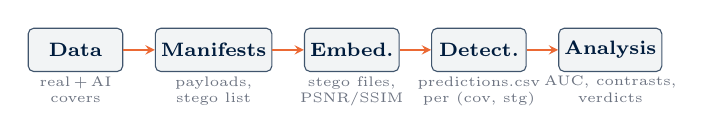
\begin{tikzpicture}[
  pstage/.style={draw=umdark!75, fill=umdark!5, rounded corners=2pt, font=\scriptsize\bfseries\color{umdark}, inner sep=2pt, minimum width=1.20cm, minimum height=0.55cm, align=center},
  pout/.style={font=\tiny\color{umgray}, align=center, inner sep=0pt},
  parrow/.style={->, >=stealth, umorange!85, line width=0.5pt},
]
\node[pstage] (data) {Data};
\node[pstage, right=0.40cm of data] (man)  {Manifests};
\node[pstage, right=0.40cm of man]  (emb)  {Embed.};
\node[pstage, right=0.40cm of emb]  (det)  {Detect.};
\node[pstage, right=0.40cm of det]  (agg)  {Analysis};
\draw[parrow] (data) -- (man);
\draw[parrow] (man)  -- (emb);
\draw[parrow] (emb)  -- (det);
\draw[parrow] (det)  -- (agg);
\node[pout, below=0.05cm of data] {real\,+\,AI\\ covers};
\node[pout, below=0.05cm of man]  {payloads,\\ stego list};
\node[pout, below=0.05cm of emb]  {stego files,\\ PSNR/SSIM};
\node[pout, below=0.05cm of det]  {predictions.csv\\ per (cov, stg)};
\node[pout, below=0.05cm of agg]  {AUC, contrasts,\\ verdicts};
\end{tikzpicture}
\caption{Five-stage pipeline. Each stage reads files written by the previous stage; manifests freeze the experimental design before any compute runs, and the analysis stage derives every contrast in this paper from a single \texttt{predictions.csv}.}
\label{fig:pipeline}
\end{figure}

\paragraph{Learned-detector training runs.} Two separate 3{,}000-group training runs were executed on a rented Vast.ai cloud instance (RTX~5880~Ada) for the SRNet and DCTR checkpoints, drawing caption~IDs disjoint from the test set. \emph{Matched training} uses the same 1:1:1 real/SDXL/FLUX factorial as the test run; \emph{real-only training} uses 9{,}000 Flickr30k captions with no AI carriers. Per-checkpoint sample count $n_\text{train}\!=\!18{,}900$, $n_\text{val}\!=\!5{,}292$ in both configurations; wall-clock $\sim\!8$~h each. Twelve checkpoints (3 SRNet + 3 DCTR per training mode) are released.

\subsection{Artefacts}
The $N\!=\!3{,}000$ test run produced 18{,}000 covers, 108{,}000 stego images, 648{,}000 classical predictions, and per-RQ verdicts (Wall-clock $\sim\!13$~h, mostly cover generation). Learned-detector inference adds $4\times108{,}000$ prediction rows kept parallel to the frozen classical predictions.

% ============================================================
\section{Classical-Detector Results}
\label{sec:results-classical}
\label{sec:results}
% ============================================================

The headline verdicts are summarised in Table~\ref{tab:verdicts}; the rest of this section walks through each RQ with the supporting figures.

\begin{table*}[t]
\centering\footnotesize
\caption{Verdict summary across the five RQs ($N\!=\!3{,}000$) at the pre-registered $\delta_\text{min}\!=\!0.05$ gate and the power-matched supplementary $0.025$ gate. Practical-count cells: $n_\text{practical}/n_\text{sig}$ with $(+\!,-)$ direction breakdown.}
\label{tab:verdicts}
\setlength{\tabcolsep}{6pt}\renewcommand{\arraystretch}{1.1}
\begin{tabular}{@{}l l c c c c c@{}}
\toprule
& & & \multicolumn{2}{c}{\textbf{$\delta_\text{min}\!=\!0.05$ (primary)}} & \multicolumn{2}{c}{\textbf{$\delta_\text{min}\!=\!0.025$ (supplementary)}} \\
\cmidrule(lr){4-5}\cmidrule(lr){6-7}
\textbf{RQ} & \textbf{Pooled $\Delta$} & \textbf{Holm sig.} & \textbf{Practical} & \textbf{Verdict} & \textbf{Practical} & \textbf{Verdict} \\
\midrule
RQ1 real vs AI        & $-0.0129$ & 16/18 & 4/16 (0,$\,$4$-$)  & mixed     & 11/16 (2,$\,$9$-$) & mixed   \\
RQ2 SDXL vs FLUX      & $+0.0004$ & 7/18  & 0/7                & trivial   & 3/7 (2,$\,$1$-$)   & \textbf{mixed} \\
RQ3 payload $\times$ source & gap shrinks with bpp & ---  & --- & supported & ---                 & supported \\
RQ4 spatial $-$ freq. & $-0.0013$ & 2/3   & 0/2                & trivial   & 1/2 (0,$\,$1$-$)   & mixed   \\
RQ5 plain vs AES      & $\sim\!0$ & 0/54 outside & ---         & supported & ---                 & supported \\
\midrule
\multicolumn{7}{@{}l@{}}{\textit{Supplementary partial AUC at FPR\,$\leq\!0.10$:}} \\
RQ1 pAUC              & $-0.0174$ & 12/18 & 6/12 (0,$\,$6$-$)  & \textbf{supported} & 9/12 (0,$\,$9$-$)  & \textbf{supported} \\
RQ2 pAUC              & $+0.0008$ & 7/18  & 1/7                & mixed     & 4/7 (3,$\,$1$-$)   & mixed   \\
\bottomrule
\end{tabular}
\end{table*}

\subsection{Headline AUC by Carrier Source and Detector}

Figure~\ref{fig:headline} plots the mean AUC of every detector against each of the three carrier sources. The visual pattern is immediate: for five of six detectors the orange/blue bars (AI carriers) are higher than the dark bars (real photographs). Only the third bar group ($\chi^2$-spatial) reverses this ordering, with real $>$ AI by a small but consistent margin.

\begin{figure*}[t]
\centering
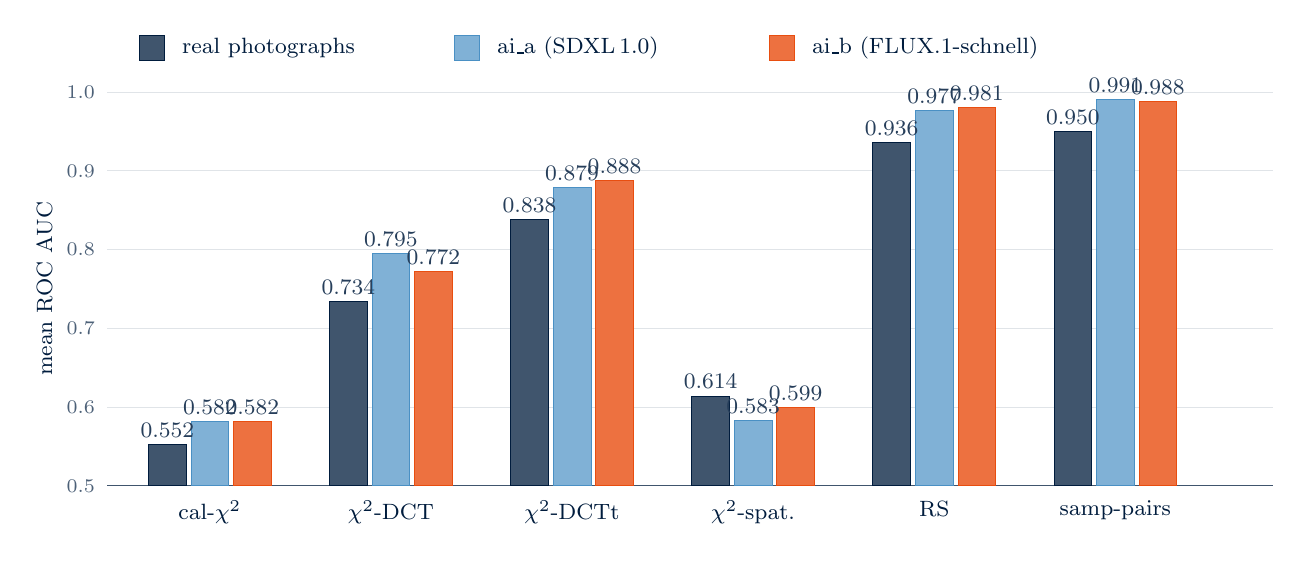
\begin{tikzpicture}[
  bargrey/.style={draw=umdark, fill=umdark!75, line width=0.25pt},
  barblue/.style={draw=umlight, fill=umlight!70, line width=0.25pt},
  baroran/.style={draw=umorange, fill=umorange!80, line width=0.25pt},
]
% y-axis (AUC 0.5..1.0 mapped to 0..5 cm)
\foreach \v in {0.5,0.6,0.7,0.8,0.9,1.0} {
  \pgfmathsetmacro{\y}{(\v - 0.5) * 10}
  \draw[umdark!12, line width=0.3pt] (0,\y) -- (14.8,\y);
  \node[font=\scriptsize\color{umdark!70}, left=1pt] at (0,\y) {\v};
}
\draw[umdark!75, line width=0.5pt] (0,0) -- (14.8,0);
\node[font=\footnotesize\color{umdark}, rotate=90] at (-0.8,2.5) {mean ROC AUC};

\def\bw{0.48}
\def\bg{0.06}
\foreach \i/\name/\real/\mla/\mlb in {%
  0/{cal-$\chi^2$}/0.552/0.582/0.582,
  1/{$\chi^2$-DCT}/0.734/0.795/0.772,
  2/{$\chi^2$-DCTt}/0.838/0.879/0.888,
  3/{$\chi^2$-spat.}/0.614/0.583/0.599,
  4/{RS}/0.936/0.977/0.981,
  5/{samp-pairs}/0.950/0.991/0.988%
} {
  \pgfmathsetmacro{\xc}{1.3 + \i*2.30}
  \pgfmathsetmacro{\xa}{\xc - 1.5*\bw - \bg}
  \pgfmathsetmacro{\xb}{\xc - 0.5*\bw}
  \pgfmathsetmacro{\xcc}{\xc + 0.5*\bw + \bg}
  \pgfmathsetmacro{\hreal}{(\real - 0.5) * 10}
  \pgfmathsetmacro{\hmla}{(\mla - 0.5) * 10}
  \pgfmathsetmacro{\hmlb}{(\mlb - 0.5) * 10}
  \draw[bargrey] (\xa,0)  rectangle (\xa+\bw,\hreal);
  \draw[barblue] (\xb,0)  rectangle (\xb+\bw,\hmla);
  \draw[baroran] (\xcc,0) rectangle (\xcc+\bw,\hmlb);
  \node[font=\footnotesize\color{umdark!85}, above=-1pt] at (\xa+\bw/2, \hreal) {\real};
  \node[font=\footnotesize\color{umdark!85}, above=-1pt] at (\xb+\bw/2, \hmla)  {\mla};
  \node[font=\footnotesize\color{umdark!85}, above=-1pt] at (\xcc+\bw/2,\hmlb) {\mlb};
  \node[font=\footnotesize\color{umdark}, below=2pt] at (\xc,0) {\name};
}
% Legend top-left
\begin{scope}[shift={(0.4, 5.4)}]
  \draw[bargrey] (0,0) rectangle (0.32,0.32); \node[font=\footnotesize\color{umdark}, right=3pt] at (0.32,0.16) {real photographs};
  \draw[barblue] (4.0,0) rectangle (4.32,0.32); \node[font=\footnotesize\color{umdark}, right=3pt] at (4.32,0.16) {ai\_a (SDXL\,1.0)};
  \draw[baroran] (8.0,0) rectangle (8.32,0.32); \node[font=\footnotesize\color{umdark}, right=3pt] at (8.32,0.16) {ai\_b (FLUX.1-schnell)};
\end{scope}
\end{tikzpicture}
\caption{Mean ROC~AUC per detector and carrier source, pooled across payload, encryption and method ($N\!=\!3{,}000$). For five of six detectors the AI bars exceed the real bar ($\Delta_\text{AUC}\!<\!0$ for each of these five); $\chi^2$-spatial alone reverses (real $>$ AI). Detector ordering left-to-right follows ascending pooled AUC. Learned-detector counterparts at the same cell are summarised in Section~\ref{sec:learnedxval} and Fig.~\ref{fig:matched-vs-realonly-heatmap}.}
\label{fig:headline}
\end{figure*}

\subsection{RQ1, Real vs.\ Pooled AI Carriers}
\label{sec:rq1}

The pooled $\Delta_\text{AUC}\!=\!-0.0129$ (95\%~CI $[-0.0137,-0.0121]$) is small but tightly constrained, with \textbf{16/18 strata} Holm-significant. At the pre-registered $\delta_\text{min}\!=\!0.05$, \textbf{4 of 16} strata clear the practical-significance gate (RS/LSB/low $-0.090$, sample-pairs/LSB/low $-0.089$, $\chi^2$-DCT-tiled/DCT/low $-0.060$, $\chi^2$-DCT/DCT/medium $-0.051$), all AI-easier across three independent detector families. The primary verdict is \textbf{mixed}: direction-consistent at the gate, most strata inside the trivial band. At the power-matched $\delta_\text{min}\!=\!0.025$ the practical count rises to 11/16 (nine AI-easier across five families plus two $\chi^2$-spatial strata reversed, medium $+0.027$, high $+0.034$); the verdict remains mixed but the evidence base is $\sim\!2.75\times\!$ deeper. The single dissenter $\chi^2$-spatial is mechanistically explained in Section~\ref{sec:chi2spatial}. Figure~\ref{fig:rq1strip} plots the 18 strata; Table~\ref{tab:rq1meta} aggregates by inverse-variance pooling per detector.

\begin{figure}[t]
\centering
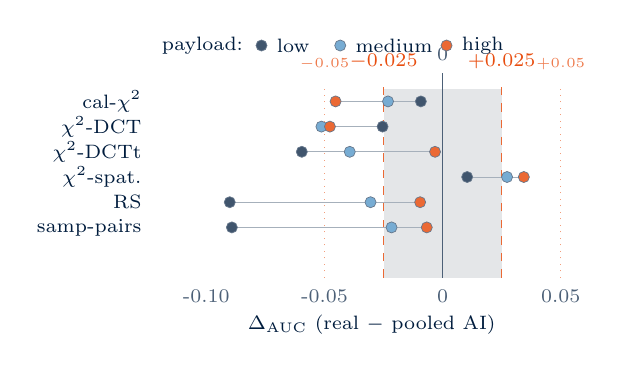
\begin{tikzpicture}[
  detrow/.style={font=\scriptsize\color{umdark}},
  dotlow/.style={circle, draw=umdark!60, fill=umdark!75,    inner sep=0pt, minimum size=4pt, line width=0.25pt},
  dotmed/.style={circle, draw=umdark!60, fill=umlight!75,   inner sep=0pt, minimum size=4pt, line width=0.25pt},
  dothigh/.style={circle, draw=umdark!60, fill=umorange!85, inner sep=0pt, minimum size=4pt, line width=0.25pt},
]
\fill[umgray!18] (2.85,-2.3) rectangle (4.35,0.10);
\draw[umdark!70, line width=0.4pt] (3.6,-2.3) -- (3.6,0.30);
\node[font=\scriptsize\color{umdark!70}, above=1pt] at (3.6,0.30) {0};
\draw[umorange!85, line width=0.4pt, dashed] (2.85,-2.3) -- (2.85,0.20);
\draw[umorange!85, line width=0.4pt, dashed] (4.35,-2.3) -- (4.35,0.20);
\node[font=\scriptsize\color{umorange}, above=1pt] at (2.85,0.20) {$-0.025$};
\node[font=\scriptsize\color{umorange}, above=1pt] at (4.35,0.20) {$+0.025$};
\draw[umorange!55, line width=0.35pt, dotted] (2.1,-2.3) -- (2.1,0.10);
\draw[umorange!55, line width=0.35pt, dotted] (5.1,-2.3) -- (5.1,0.10);
\node[font=\tiny\color{umorange!75}] at (2.1,0.42) {$-0.05$};
\node[font=\tiny\color{umorange!75}] at (5.1,0.42) {$+0.05$};
\foreach \v in {-0.10,-0.05,0,0.05} {
  \pgfmathsetmacro{\x}{(\v + 0.12) * 30}
  \node[font=\scriptsize\color{umdark!70}, below=1pt] at (\x,-2.3) {\v};
}
\node[font=\scriptsize\color{umdark}, below=10pt] at (2.7,-2.3) {$\Delta_\text{AUC}$ (real $-$ pooled AI)};

\foreach \i/\labl/\dl/\dm/\dh in {%
  0/{cal-$\chi^2$}/-0.0092/-0.0231/-0.0453,
  1/{$\chi^2$-DCT}/-0.0254/-0.0513/-0.0477,
  2/{$\chi^2$-DCTt}/-0.0596/-0.0393/-0.0032,
  3/{$\chi^2$-spat.}/0.0104/0.0273/0.0344,
  4/{RS}/-0.0901/-0.0305/-0.0095,
  5/{samp-pairs}/-0.0892/-0.0216/-0.0067%
} {
  \pgfmathsetmacro{\y}{-\i*0.32 - 0.06}
  \node[detrow, anchor=east] at (-0.10,\y) {\labl};
  \pgfmathsetmacro{\xa}{(\dl + 0.12) * 30}
  \pgfmathsetmacro{\xb}{(\dm + 0.12) * 30}
  \pgfmathsetmacro{\xcc}{(\dh + 0.12) * 30}
  \draw[umdark!35, line width=0.35pt] (\xa,\y) -- (\xcc,\y);
  \node[dotlow]  at (\xa,\y) {};
  \node[dotmed]  at (\xb,\y) {};
  \node[dothigh] at (\xcc,\y) {};
}
\node[font=\scriptsize\color{umdark}] at (0.55,0.65) {payload:};
\node[dotlow]  at (1.30,0.65) {};
\node[font=\scriptsize\color{umdark}, right=2pt] at (1.30,0.65) {low};
\node[dotmed]  at (2.30,0.65) {};
\node[font=\scriptsize\color{umdark}, right=2pt] at (2.30,0.65) {medium};
\node[dothigh] at (3.65,0.65) {};
\node[font=\scriptsize\color{umdark}, right=2pt] at (3.65,0.65) {high};
\end{tikzpicture}
\caption{RQ1, paired DeLong $\Delta_\text{AUC}$ per stratum (real $-$ pooled AI), classical detectors. Grey band: supplementary $|\Delta|\!<\!0.025$; dotted lines: pre-registered $\pm 0.05$. Learned-detector counterpart in Fig.~\ref{fig:matched-vs-realonly-heatmap} and Fig.~\ref{fig:learned-payload-trend}.}
\label{fig:rq1strip}
\end{figure}

\begin{table}[t]
\centering\small
\caption{RQ1, per-detector inverse-variance pooled $\Delta_\text{AUC}$ across the three payload strata ($k\!=\!3$). All meta values negative except $\chi^2$-spatial.}
\label{tab:rq1meta}
\setlength{\tabcolsep}{5pt}\renewcommand{\arraystretch}{1.1}
\begin{tabular}{@{}l r l@{}}
\toprule
\textbf{Detector} & \textbf{Pooled $\Delta$} & \textbf{95\% CI} \\
\midrule
calibration $\chi^2$    & $-0.026$ & $[-0.033, -0.019]$ \\
$\chi^2$-DCT            & $-0.045$ & $[-0.050, -0.040]$ \\
$\chi^2$-DCT-tiled      & $-0.006$ & $[-0.008, -0.005]$ \\
$\chi^2$-spatial        & $+0.025$ & $[+0.018, +0.032]$ \\
RS                      & $-0.015$ & $[-0.016, -0.014]$ \\
sample-pairs            & $-0.014$ & $[-0.015, -0.012]$ \\
\midrule
\textbf{All strata}     & $\boldsymbol{-0.013}$ & $\boldsymbol{[-0.014, -0.012]}$ \\
\bottomrule
\end{tabular}
\end{table}

\subsection{RQ2, SDXL vs.\ FLUX within AI}

The pooled $\Delta_\text{AUC}\!=\!+0.0004$ is essentially zero. 7/18 strata are Holm-significant under the larger sample size, and the strata are mixed in direction (four favour SDXL, three FLUX). At the pre-registered $\delta_\text{min}\!=\!0.05$, \textbf{none of the seven Holm-significant strata clear the practical-significance gate}, the primary verdict is \textbf{trivial} (Figure~\ref{fig:rq2}). At the supplementary $\delta_\text{min}\!=\!0.025$, three strata clear the tighter gate ($\chi^2$-DCT/dct/medium $+0.031$, $\chi^2$-DCT/dct/high $+0.025$, $\chi^2$-spatial/LSB/high $-0.029$), so the verdict shifts to \textbf{mixed}; however, no detector family is unanimous across payloads, so the directional-consistency criterion that would support a "generator effect" claim still fails.

\begin{figure}[t]
\centering
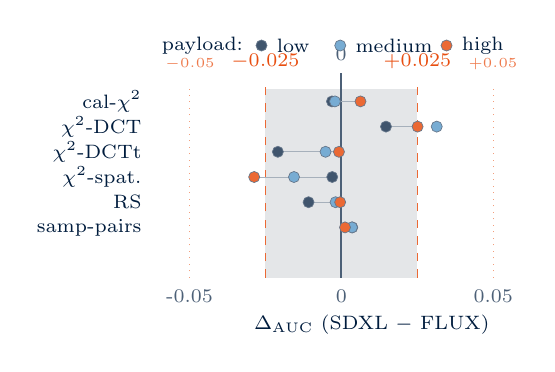
\begin{tikzpicture}[
  detrow/.style={font=\scriptsize\color{umdark}},
  dotlow/.style={circle, draw=umdark!60, fill=umdark!75,    inner sep=0pt, minimum size=4pt, line width=0.25pt},
  dotmed/.style={circle, draw=umdark!60, fill=umlight!75,   inner sep=0pt, minimum size=4pt, line width=0.25pt},
  dothigh/.style={circle, draw=umdark!60, fill=umorange!85, inner sep=0pt, minimum size=4pt, line width=0.25pt},
]
% RQ2 scale: Δ in [-0.06, +0.08] -> [0, 5.4] cm.
% ± 0.025 lives at x = 1.35 / 3.28; ± 0.05 lives at x = 0.39 / 4.24
\fill[umgray!18] (1.35,-2.3) rectangle (3.28,0.10);
\draw[umdark!70, line width=0.4pt] (2.31,-2.3) -- (2.31,0.30);
\node[font=\scriptsize\color{umdark!70}, above=1pt] at (2.31,0.30) {0};
\draw[umorange!85, line width=0.4pt, dashed] (1.35,-2.3) -- (1.35,0.20);
\draw[umorange!85, line width=0.4pt, dashed] (3.28,-2.3) -- (3.28,0.20);
\node[font=\scriptsize\color{umorange}, above=1pt] at (1.35,0.20) {$-0.025$};
\node[font=\scriptsize\color{umorange}, above=1pt] at (3.28,0.20) {$+0.025$};
\draw[umorange!55, line width=0.35pt, dotted] (0.39,-2.3) -- (0.39,0.10);
\draw[umorange!55, line width=0.35pt, dotted] (4.24,-2.3) -- (4.24,0.10);
\node[font=\tiny\color{umorange!75}] at (0.39,0.42) {$-0.05$};
\node[font=\tiny\color{umorange!75}] at (4.24,0.42) {$+0.05$};
\foreach \v in {-0.05,0,0.05} {
  \pgfmathsetmacro{\x}{(\v + 0.06) / 0.14 * 5.4}
  \node[font=\scriptsize\color{umdark!70}, below=1pt] at (\x,-2.3) {\v};
}
\node[font=\scriptsize\color{umdark}, below=10pt] at (2.7,-2.3) {$\Delta_\text{AUC}$ (SDXL $-$ FLUX)};

\foreach \i/\labl/\dl/\dm/\dh in {%
  0/{cal-$\chi^2$}/-0.0031/-0.0021/0.0063,
  1/{$\chi^2$-DCT}/0.0147/0.0314/0.0251,
  2/{$\chi^2$-DCTt}/-0.0209/-0.0052/-0.0008,
  3/{$\chi^2$-spat.}/-0.0030/-0.0156/-0.0287,
  4/{RS}/-0.0108/-0.0019/-0.0004,
  5/{samp-pairs}/0.0036/0.0035/0.0012%
} {
  \pgfmathsetmacro{\y}{-\i*0.32 - 0.06}
  \node[detrow, anchor=east] at (-0.10,\y) {\labl};
  \pgfmathsetmacro{\xa}{(\dl + 0.06) / 0.14 * 5.4}
  \pgfmathsetmacro{\xb}{(\dm + 0.06) / 0.14 * 5.4}
  \pgfmathsetmacro{\xcc}{(\dh + 0.06) / 0.14 * 5.4}
  \draw[umdark!35, line width=0.35pt] (\xa,\y) -- (\xcc,\y);
  \node[dotlow]  at (\xa,\y) {};
  \node[dotmed]  at (\xb,\y) {};
  \node[dothigh] at (\xcc,\y) {};
}
\node[font=\scriptsize\color{umdark}] at (0.55,0.65) {payload:};
\node[dotlow]  at (1.30,0.65) {};
\node[font=\scriptsize\color{umdark}, right=2pt] at (1.30,0.65) {low};
\node[dotmed]  at (2.30,0.65) {};
\node[font=\scriptsize\color{umdark}, right=2pt] at (2.30,0.65) {medium};
\node[dothigh] at (3.65,0.65) {};
\node[font=\scriptsize\color{umdark}, right=2pt] at (3.65,0.65) {high};
\end{tikzpicture}
\caption{RQ2, paired DeLong $\Delta_\text{AUC}$ per stratum (SDXL $-$ FLUX), classical detectors. Grey band: $|\Delta|\!<\!0.025$; dotted lines: pre-registered $\pm 0.05$. No detector family is unanimous across payloads. Learned-detector counterpart in Fig.~\ref{fig:learned-payload-trend}.}
\label{fig:rq2}
\end{figure}

\begin{table}[t]
\centering\small
\caption{RQ2, per-detector inverse-variance pooled $\Delta_\text{AUC}$ (SDXL $-$ FLUX). All CIs are an order of magnitude tighter than $\delta_\text{min}\!=\!0.05$; no detector clears the practical-significance gate.}
\label{tab:rq2meta}
\setlength{\tabcolsep}{5pt}\renewcommand{\arraystretch}{1.1}
\begin{tabular}{@{}l r l@{}}
\toprule
\textbf{Detector} & \textbf{Pooled $\Delta$} & \textbf{95\% CI} \\
\midrule
calibration $\chi^2$    & $+0.001$ & $[-0.008, +0.009]$ \\
$\chi^2$-DCT            & $+0.025$ & $[+0.020, +0.030]$ \\
$\chi^2$-DCT-tiled      & $-0.001$ & $[-0.002, -0.000]$ \\
$\chi^2$-spatial        & $-0.016$ & $[-0.024, -0.008]$ \\
RS                      & $-0.001$ & $[-0.001, -0.000]$ \\
sample-pairs            & $+0.001$ & $[+0.001, +0.002]$ \\
\midrule
\textbf{All strata}     & $\boldsymbol{+0.000}$ & $\boldsymbol{[+0.000, +0.001]}$ \\
\bottomrule
\end{tabular}
\end{table}

The two diffusion models are functionally interchangeable at the detector level, and the proposal-driven model swap from PixArt-$\alpha$ to FLUX.1-schnell did not bias the result.

\subsection{RQ3, Payload Interaction}

The pooled real$-$AI gap is monotone in payload: $-0.0486 \to -0.0281 \to -0.0157$ at low/medium/high. The carrier-source signal is strongest at low payload, where the embedding is subtle enough that cover-side statistics carry the discriminative weight; at high payload the per-pixel modification noise dominates and the source fingerprint is overwhelmed.

\begin{figure}[t]
\centering
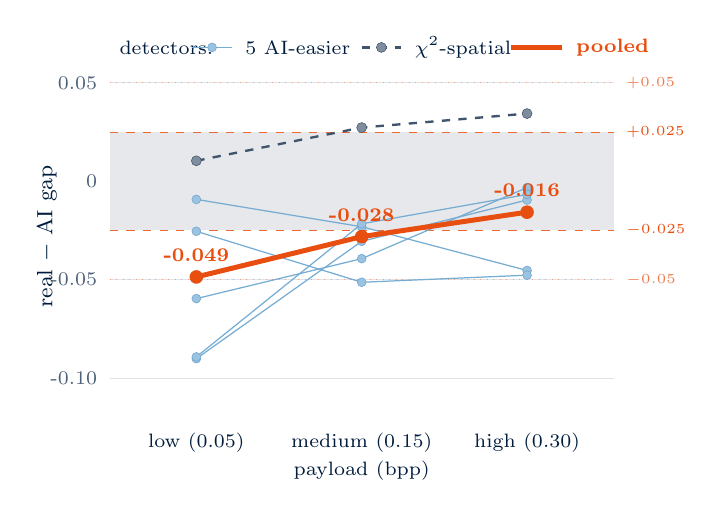
\begin{tikzpicture}[
  detlineA/.style={line width=0.45pt, draw=umlight!75},
  detlineC/.style={line width=0.85pt, draw=umdark!75, dashed},
  pooledline/.style={line width=1.8pt, draw=umorange},
  detmarkA/.style={circle, draw=umlight!80, fill=umlight!55, inner sep=0pt, minimum size=3.2pt, line width=0.2pt},
  detmarkC/.style={circle, draw=umdark!75, fill=umdark!50,   inner sep=0pt, minimum size=3.6pt, line width=0.2pt},
]
\def\xL{0}\def\xR{6.4}
\def\xlow{1.1}\def\xmed{3.2}\def\xhigh{5.3}
% y-grid: real-AI gap in [-0.12, 0.05] -> y = (val+0.12)*25
\foreach \v in {-0.10,-0.05,0,0.05} {
  \pgfmathsetmacro{\y}{(\v + 0.12) * 25}
  \draw[umdark!12, line width=0.3pt] (\xL,\y) -- (\xR,\y);
  \node[font=\scriptsize\color{umdark!70}, left=1pt] at (\xL,\y) {\v};
}
\pgfmathsetmacro{\yzero}{(0 + 0.12) * 25}
\draw[umdark!70, line width=0.4pt] (\xL,\yzero) -- (\xR,\yzero);
% Supplementary trivial band |gap|<0.025 (grey fill)
\pgfmathsetmacro{\ylotwohalf}{(-0.025 + 0.12) * 25}
\pgfmathsetmacro{\yhitwohalf}{(0.025 + 0.12) * 25}
\fill[umgray!16] (\xL,\ylotwohalf) rectangle (\xR,\yhitwohalf);
\draw[umorange!85, line width=0.4pt, dashed] (\xL,\ylotwohalf) -- (\xR,\ylotwohalf);
\draw[umorange!85, line width=0.4pt, dashed] (\xL,\yhitwohalf) -- (\xR,\yhitwohalf);
\node[font=\tiny\color{umorange}, right=1pt] at (\xR,\ylotwohalf) {$-0.025$};
\node[font=\tiny\color{umorange}, right=1pt] at (\xR,\yhitwohalf) {$+0.025$};
% Pre-registered ±0.05 reference lines (dotted)
\pgfmathsetmacro{\ylofive}{(-0.05 + 0.12) * 25}
\pgfmathsetmacro{\yhifive}{(0.05 + 0.12) * 25}
\draw[umorange!55, line width=0.35pt, dotted] (\xL,\ylofive) -- (\xR,\ylofive);
\draw[umorange!55, line width=0.35pt, dotted] (\xL,\yhifive) -- (\xR,\yhifive);
\node[font=\tiny\color{umorange!75}, right=1pt] at (\xR,\ylofive) {$-0.05$};
\node[font=\tiny\color{umorange!75}, right=1pt] at (\xR,\yhifive) {$+0.05$};

\node[font=\scriptsize\color{umdark}, below=2pt] at (\xlow,0)  {low (0.05)};
\node[font=\scriptsize\color{umdark}, below=2pt] at (\xmed,0)  {medium (0.15)};
\node[font=\scriptsize\color{umdark}, below=2pt] at (\xhigh,0) {high (0.30)};
\node[font=\scriptsize\color{umdark}, below=12pt] at (\xmed,0) {payload (bpp)};
\node[font=\footnotesize\color{umdark}, rotate=90] at (-0.8,2.3) {real $-$ AI gap};

% 5 AI-easier detector lines (cal-chi2, chi2-DCT, chi2-DCT-tiled, RS, sample_pairs)
\foreach \ll/\mm/\hh in {%
  -0.0092/-0.0231/-0.0453,
  -0.0254/-0.0513/-0.0477,
  -0.0596/-0.0393/-0.0032,
  -0.0901/-0.0305/-0.0095,
  -0.0892/-0.0216/-0.0067%
} {
  \pgfmathsetmacro{\ya}{(\ll + 0.12) * 25}
  \pgfmathsetmacro{\yb}{(\mm + 0.12) * 25}
  \pgfmathsetmacro{\yc}{(\hh + 0.12) * 25}
  \draw[detlineA] (\xlow,\ya) -- (\xmed,\yb) -- (\xhigh,\yc);
  \node[detmarkA] at (\xlow,\ya)  {};
  \node[detmarkA] at (\xmed,\yb)  {};
  \node[detmarkA] at (\xhigh,\yc) {};
}
% chi-spatial outlier (dashed dark)
{
  \pgfmathsetmacro{\ya}{(0.0104 + 0.12) * 25}
  \pgfmathsetmacro{\yb}{(0.0273 + 0.12) * 25}
  \pgfmathsetmacro{\yc}{(0.0344 + 0.12) * 25}
  \draw[detlineC] (\xlow,\ya) -- (\xmed,\yb) -- (\xhigh,\yc);
  \node[detmarkC] at (\xlow,\ya)  {};
  \node[detmarkC] at (\xmed,\yb)  {};
  \node[detmarkC] at (\xhigh,\yc) {};
}
% Pooled bold orange line
\pgfmathsetmacro{\yp}{(-0.0486 + 0.12) * 25}
\pgfmathsetmacro{\yq}{(-0.0281 + 0.12) * 25}
\pgfmathsetmacro{\yr}{(-0.0157 + 0.12) * 25}
\draw[pooledline] (\xlow,\yp) -- (\xmed,\yq) -- (\xhigh,\yr);
\node[circle, draw=umorange, fill=umorange, inner sep=0pt, minimum size=4.5pt] at (\xlow,\yp)  {};
\node[circle, draw=umorange, fill=umorange, inner sep=0pt, minimum size=4.5pt] at (\xmed,\yq)  {};
\node[circle, draw=umorange, fill=umorange, inner sep=0pt, minimum size=4.5pt] at (\xhigh,\yr) {};
\node[font=\scriptsize\color{umorange}\bfseries, above=2pt] at (\xlow,\yp) {-0.049};
\node[font=\scriptsize\color{umorange}\bfseries, above=2pt] at (\xmed,\yq) {-0.028};
\node[font=\scriptsize\color{umorange}\bfseries, above=2pt] at (\xhigh,\yr) {-0.016};

% Legend
\node[font=\scriptsize\color{umdark}, anchor=west] at (0.0, 4.7) {detectors:};
\draw[detlineA] (1.05,4.7) -- (1.55,4.7); \node[detmarkA] at (1.30,4.7) {};
\node[font=\scriptsize\color{umdark}, anchor=west] at (1.60,4.7) {5 AI-easier};
\draw[detlineC] (3.20,4.7) -- (3.70,4.7); \node[detmarkC] at (3.45,4.7) {};
\node[font=\scriptsize\color{umdark}, anchor=west] at (3.75,4.7) {$\chi^2$-spatial};
\draw[pooledline] (5.10,4.7) -- (5.75,4.7);
\node[font=\scriptsize\color{umorange}\bfseries, anchor=west] at (5.80,4.7) {pooled};
\end{tikzpicture}
\caption{RQ3, real-minus-AI AUC gap vs.\ payload, classical detectors. Grey band: $|\text{gap}|\!<\!0.025$; dotted lines: $\pm 0.05$. Pooled gap shrinks monotonically with payload. Learned-detector counterpart with both training configurations in Fig.~\ref{fig:learned-payload-trend}.}
\label{fig:rq3}
\end{figure}

Verdict: \textbf{supported}. The monotone decrease in gap magnitude with payload is the most operationally relevant finding of the study, because low payloads are exactly the regime a forensic analyst cares about (large payloads are easy to detect on either carrier).

\subsection{RQ4, Spatial vs.\ Frequency Branch Interaction}
\label{sec:rq4}

We compute $\Delta\Delta_\text{AUC}\!=\!\text{(spatial gap)}-\text{(frequency gap)}$ per payload level. The pooled estimate is $-0.0013$ (95\%~CI $[-0.0031,+0.0005]$), which spans zero. The per-payload pattern is informative even though the pooled summary is null:

\begin{center}\small
\begin{tabular}{lrrr}
\textbf{payload} & \textbf{spatial gap} & \textbf{frequency gap} & $\boldsymbol{\Delta\Delta}$ \\
\midrule
low    & $-0.076$ & $-0.033$ & $-0.043$ \\
medium & $-0.024$ & $-0.039$ & $+0.015$ \\
high   & $-0.008$ & $-0.007$ & $-0.001$ \\
\end{tabular}
\end{center}

Spatial-branch dominates at low payload, frequency-branch at medium, tie at high (Figure~\ref{fig:rq4}); the per-payload pattern is identical to the $N\!=\!1{,}000$ result, but the larger sample tightens the pooled $\Delta\Delta$ to within zero.

\begin{figure}[t]
\centering
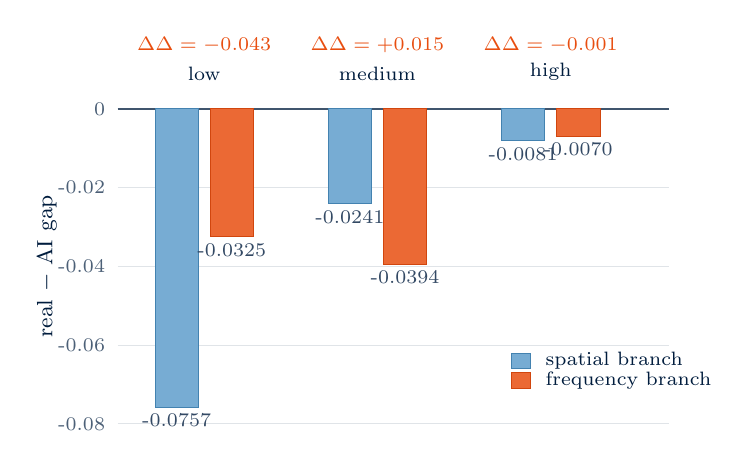
\begin{tikzpicture}[
  barlabel/.style={font=\scriptsize\color{umdark!80}},
  barspat/.style={draw=umlight!90!black, fill=umlight!75, line width=0.25pt},
  barfreq/.style={draw=umorange!90!black, fill=umorange!85, line width=0.25pt},
]
\def\xL{0}\def\xR{7.0}
\foreach \v in {-0.08,-0.06,-0.04,-0.02,0} {
  \pgfmathsetmacro{\y}{\v * 50}
  \draw[umdark!12, line width=0.3pt] (\xL,\y) -- (\xR,\y);
  \node[font=\scriptsize\color{umdark!70}, left=1pt] at (\xL,\y) {\v};
}
\draw[umdark!75, line width=0.5pt] (\xL,0) -- (\xR,0);
\node[font=\footnotesize\color{umdark}, rotate=90] at (-0.9,-2) {real $-$ AI gap};

\def\bw{0.55}
\def\bg{0.15}
\foreach \i/\pl/\spat/\freq/\dd in {%
  0/{low}/-0.0757/-0.0325/{-0.043},
  1/{medium}/-0.0241/-0.0394/{+0.015},
  2/{high}/-0.0081/-0.0070/{-0.001}%
} {
  \pgfmathsetmacro{\xc}{1.1 + \i*2.20}
  \pgfmathsetmacro{\xa}{\xc - 0.5*\bw - \bg/2}
  \pgfmathsetmacro{\xb}{\xc + 0.5*\bw + \bg/2}
  \pgfmathsetmacro{\hspat}{\spat * 50}
  \pgfmathsetmacro{\hfreq}{\freq * 50}
  \draw[barspat] (\xa-\bw/2,0) rectangle (\xa+\bw/2,\hspat);
  \draw[barfreq] (\xb-\bw/2,0) rectangle (\xb+\bw/2,\hfreq);
  \node[barlabel, below=-1pt] at (\xa,\hspat) {\spat};
  \node[barlabel, below=-1pt] at (\xb,\hfreq) {\freq};
  \node[font=\scriptsize\color{umdark}, above=4pt] at (\xc,0.10) {\pl};
  \node[font=\scriptsize\color{umorange}\bfseries, above=14pt] at (\xc,0.10) {$\Delta\Delta=\dd$};
}
% Legend
\begin{scope}[shift={(5.0, -3.6)}]
  \draw[barspat] (0,0.30) rectangle (0.24,0.50);
  \draw[barfreq] (0,0.05) rectangle (0.24,0.25);
  \node[font=\scriptsize\color{umdark}, right=2pt] at (0.24,0.40) {spatial branch};
  \node[font=\scriptsize\color{umdark}, right=2pt] at (0.24,0.15) {frequency branch};
\end{scope}
\end{tikzpicture}
\caption{RQ4, per-payload spatial vs.\ frequency branch source gap, classical detectors. $\Delta\Delta$ positive $=$ frequency branch has the larger source effect. The dominant branch flips with payload; pooled $\Delta\Delta\!=\!-0.001$. Learned-detector counterpart in Fig.~\ref{fig:learned-payload-trend}.}
\label{fig:rq4}
\end{figure}

Verdict: \textbf{trivial}. The per-payload pattern is a candidate exploratory finding for follow-up work; the pooled summary is honestly null.

\subsection{RQ5, Encryption Invariance}
\label{sec:rq5}

All 54/54 strata fall inside the $\pm0.025$ AUC equivalence margin (pooled $|\Delta_\text{AUC}|\!<\!10^{-6}$). Verdict: \textbf{supported}, the expected null (Figure~\ref{fig:rq5}); the learned-detector cross-validation matches (Table~\ref{tab:learned-verdicts}, 18/18 strata within margin), the substitution of random/plain payloads for AES-encrypted real payloads is empirically validated under both detector families.

\begin{figure}[t]
\centering
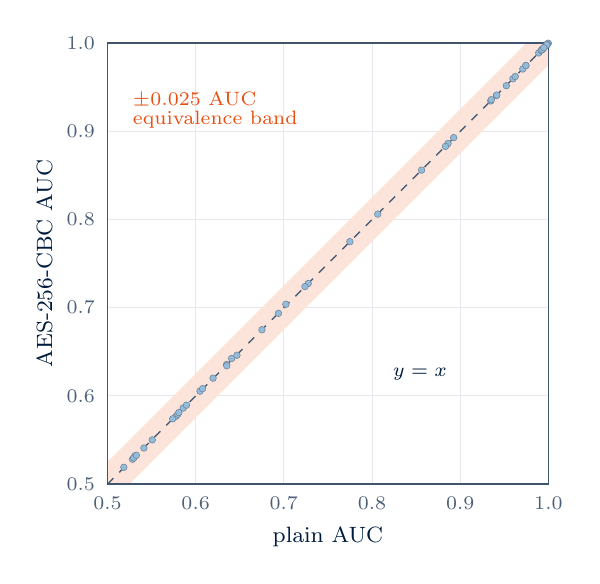
\begin{tikzpicture}[
  pt/.style={circle, draw=umdark!55, fill=umlight!60, inner sep=0pt, minimum size=2.4pt, line width=0.20pt},
]
\def\sz{5.6}
\foreach \v in {0.5,0.6,0.7,0.8,0.9,1.0} {
  \pgfmathsetmacro{\xy}{(\v - 0.5) * 11.2}
  \draw[umdark!10, line width=0.3pt] (0,\xy) -- (\sz,\xy);
  \draw[umdark!10, line width=0.3pt] (\xy,0) -- (\xy,\sz);
  \node[font=\scriptsize\color{umdark!70}, left=1pt] at (0,\xy) {\v};
  \node[font=\scriptsize\color{umdark!70}, below=1pt] at (\xy,0) {\v};
}
\fill[umorange!15] (0,0.28) -- (5.32,5.6) -- (5.6,5.6) -- (5.6,5.32) -- (0.28,0) -- (0,0) -- cycle;
\draw[umdark!70, line width=0.5pt, dashed] (0,0) -- (\sz,\sz);
\draw[umdark!75, line width=0.5pt] (0,0) rectangle (\sz,\sz);
\node[font=\footnotesize\color{umdark}, below=12pt] at (\sz/2,0) {plain AUC};
\node[font=\footnotesize\color{umdark}, rotate=90] at (-0.8,\sz/2) {AES-256-CBC AUC};

\foreach \px/\py in {%
  0.6408/0.6424, 0.6351/0.6356, 0.5859/0.5862, 0.5284/0.5282, 0.5310/0.5318, 0.5186/0.5190,
  0.5779/0.5769, 0.5798/0.5792, 0.5508/0.5501, 0.9598/0.9596, 0.9347/0.9345, 0.8926/0.8929,
  0.6197/0.6201, 0.6050/0.6054, 0.5810/0.5811, 0.8065/0.8061, 0.7749/0.7749, 0.7276/0.7274,
  0.9969/0.9970, 0.9979/0.9977, 0.9929/0.9932, 0.7023/0.7039, 0.7239/0.7240, 0.6353/0.6342,
  0.9352/0.9359, 0.9410/0.9405, 0.8862/0.8862, 0.6468/0.6461, 0.6752/0.6750, 0.6939/0.6936,
  0.5298/0.5296, 0.5328/0.5326, 0.5413/0.5409, 0.5740/0.5740, 0.5896/0.5895, 0.6079/0.6082,
  0.9983/0.9983, 0.9987/0.9987, 0.9890/0.9889, 0.9414/0.9411, 0.9523/0.9517, 0.8562/0.8560,
  0.9917/0.9917, 0.9938/0.9934, 0.9624/0.9622, 0.9999/0.9999, 0.9988/0.9988, 0.9927/0.9924,
  0.9744/0.9746, 0.9710/0.9707, 0.8833/0.8829, 0.9981/0.9981, 0.9947/0.9947, 0.9746/0.9747%
} {
  \pgfmathsetmacro{\xx}{(\px - 0.5) * 11.2}
  \pgfmathsetmacro{\yy}{(\py - 0.5) * 11.2}
  \node[pt] at (\xx,\yy) {};
}
\node[font=\scriptsize\color{umorange}, anchor=south west] at (0.20, 4.65) {$\pm 0.025$ AUC};
\node[font=\scriptsize\color{umorange}, anchor=south west] at (0.20, 4.40) {equivalence band};
\node[font=\scriptsize\color{umdark}, anchor=south west] at (3.5,1.2) {$y = x$};
\end{tikzpicture}
\caption{RQ5, plain vs.\ AES-256-CBC stego AUC, all 54 strata (6 detectors $\times$ 3 sources $\times$ 3 payloads). Every point sits inside the $\pm 0.025$ AUC equivalence band; the detectors react to embedding distortion, not plaintext patterns.}
\label{fig:rq5}
\end{figure}

The clean negative result also validates the embedding pipeline: a non-null here would have indicated that detectors were reacting to payload-bit regularity rather than to LSB-flip artefacts.

\subsection{Stego Image Quality and Supplementary Partial-AUC}
Per-source mean PSNR (factorial mean across method/payload/encryption) is $58$--$59$~dB (real $58.2$~dB, SDXL/FLUX $59.2$~dB; SSIM $\geq\!0.999$ everywhere), well above the imperceptibility floor and ruling out distortion-mismatch as an AUC-contrast explanation; the DCT branch shows a $\sim\!2$~dB per-source gap consistent with the RQ1 interpretation (Appendix~\ref{app:quality} for full table). The partial-AUC view at FPR\,$\leq\!0.10$ (Appendix~\ref{app:pauc}) sharpens every effect: the RQ1 pooled $\Delta_\text{pAUC}\!=\!-0.0174$ (vs.\ $-0.0129$ at full AUC) and 6 of 12 Holm-significant strata clear the pre-registered $\delta_\text{min}\!=\!0.05$ gate, strengthening the RQ1 verdict from mixed to \textbf{supported}. Conversely, every $\chi^2$-spatial pAUC contrast has $|\Delta|\!\leq\!0.007$ and is non-significant, the full-AUC reversal we observed for that detector \emph{dissolves} in the operational FPR regime, which we revisit in Section~\ref{sec:chi2spatial}.

% ============================================================
\section{Learned-Detector Cross-Validation}
\label{sec:learnedxval}
% ============================================================

This section applies the pre-registered statistical protocol of Section~\ref{sec:stats} (paired DeLong, Bonferroni--Holm at $\alpha\!=\!0.05$, $\delta_\text{min}$ thresholds at 0.05 primary / 0.025 supplementary, equivalence test at $\pm 0.025$ for RQ5) to two state-of-the-art learned detectors, SRNet (spatial) and DCTR (frequency), as an independent replication of the classical findings on an orthogonal detector family. The Bonferroni--Holm family is computed separately for the six learned-detector strata, leaving the pre-registered classical-detector correction (Table~\ref{tab:verdicts}) untouched.

\paragraph{Two complementary training configurations.} We report two learned-detector training runs that share architecture, hyperparameters, and per-checkpoint sample budget but differ in their training-corpus carrier distribution:

\begin{itemize}
\item \textbf{Matched training}: the training corpus's carrier-source distribution matches the test corpus's (real + SDXL + FLUX, 1:1:1). \emph{Question answered}: given equal training exposure to all carrier sources, do learned detectors show source-correlated performance differences on the test set?
\item \textbf{Real-only training}: the training corpus is restricted to real Flickr30k captions; the AI sources are held out from training but still appear in the test set. \emph{Question answered}: if the detector is trained without seeing the AI carrier sources at all (the realistic deployment scenario where AI carriers post-date the training corpus), does it still generalise to them?
\end{itemize}

\noindent Neither configuration is `the' learned-detector analysis: matched training is the pre-registered confirmatory cross-validation of the classical findings under a controlled, equal-exposure regime; real-only training is a within-paper ablation that disentangles architectural source-invariance from balanced-training-exposure artefact in the matched-training result. The contrast between the two is what supports the strongest claim in this section.

\subsection{Training Outcomes and Test-Set AUCs (matched training)}
\label{sec:v1-train}

The matched-training corpus is the 3{,}000-caption source-balanced run of Section~\ref{sec:experiments} (real + SDXL + FLUX, 1:1:1; per-checkpoint $n_\text{train}\!=\!18{,}900$, $n_\text{val}\!=\!5{,}292$). All six checkpoints converged within budget. Validation AUCs: SRNet $\{0.9989, 0.9988, 0.9990\}$ at LSB / \{low, medium, high\}; DCTR $\{0.6174, 0.7949, 0.9363\}$ at DCT / \{low, medium, high\}. Applying the checkpoints as-is to the held-out test set (leakage-guarded by manifest hash; Section~\ref{sec:learned-detectors}) gives the per-source AUCs of Table~\ref{tab:learned-headline-auc}. SRNet saturates the LSB-detection task at AUC$\geq$0.997 across all carriers, payloads and encryption modes, substantially above the strongest classical LSB detector (sample\_pairs at 0.93 overall). DCTR sits at AUC 0.81 overall, between $\chi^2$-DCT-tiled (0.85) and $\chi^2$-DCT (0.76); its per-cell range from 0.62 (low payload) to 0.94 (high payload) tracks the payload signal cleanly.

\begin{table}[!htbp]
\centering\footnotesize
\caption{Matched-training learned-detector test AUC per (detector, payload, carrier). AI-A$=$SDXL, AI-B$=$FLUX; encryption averaged. Overall: SRNet 0.998, DCTR 0.814.}
\label{tab:learned-headline-auc}
\setlength{\tabcolsep}{5pt}\renewcommand{\arraystretch}{1.05}
\begin{tabular}{@{}llrrr@{}}
\toprule
\textbf{Det.} & \textbf{Cell} & \textbf{Real} & \textbf{AI-A} & \textbf{AI-B} \\
\midrule
SRNet & low     & 0.9990 & 0.9965 & 0.9985 \\
SRNet & medium  & 0.9992 & 0.9981 & 0.9981 \\
SRNet & high    & 0.9994 & 0.9985 & 0.9978 \\
DCTR  & low     & 0.6043 & 0.6453 & 0.6233 \\
DCTR  & medium  & 0.7831 & 0.8302 & 0.7911 \\
DCTR  & high    & 0.9300 & 0.9577 & 0.9317 \\
\bottomrule
\end{tabular}
\end{table}

\subsection{Per-RQ Cross-Validation Verdicts}

Table~\ref{tab:learned-verdicts} and the matched visual in Figure~\ref{fig:learned-verdicts} report the learned-detector verdict for each RQ alongside the corresponding classical-detector verdict, with the three-way interpretation \textbf{corroborates / refines / contradicts}.

\begin{table}[!htbp]
\centering\footnotesize
\caption{Cross-validation verdicts. Classical and learned pooled $\Delta_\text{AUC}$ per RQ; matched-training-learned column.}
\label{tab:learned-verdicts}
\setlength{\tabcolsep}{3pt}\renewcommand{\arraystretch}{1.05}
\begin{tabular}{@{}lccl@{}}
\toprule
\textbf{RQ} & \textbf{Classical $\Delta$} & \textbf{Learned $\Delta$} & \textbf{Verdict} \\
\midrule
RQ1     & $-0.0129$ mix.   & $+0.0012$ triv.  & Contradicts$^\star$ \\
RQ2     & $+0.0004$ triv.  & $-0.0002$ triv.  & Corrob.\ \\
RQ3     & $-0.0157$ supp.  & $-0.0068$ mix.   & Refines (1/2) \\
RQ4     & $-0.0013$ triv.  & $+0.0159$ triv.  & Corrob.\ \\
RQ5     & $\approx 0$ supp.\ & $\approx 0$ supp.\ & Corrob.\ \\
\bottomrule
\end{tabular}\\[1pt]
{\scriptsize $^\star$\,inverse-variance pooling artefact (SRNet at ceiling dominates the pool); per-detector reading, DCTR alone gives $-0.030$, corroborating classical.}
\end{table}

\begin{figure}[!htbp]
\centering
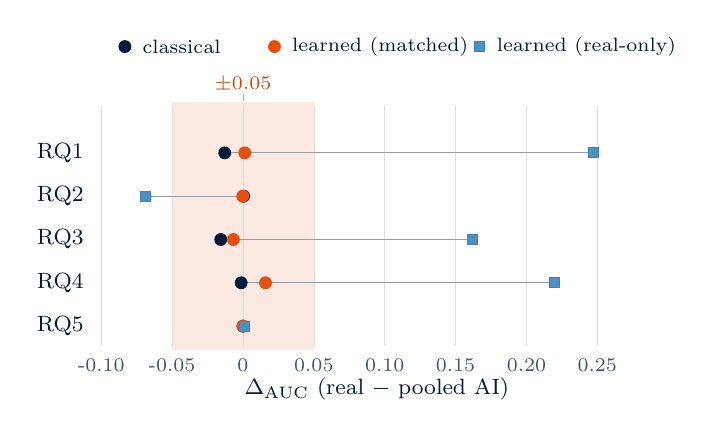
\begin{tikzpicture}[
  classDot/.style ={circle,    draw=umdark,   fill=umdark,   inner sep=1.5pt},
  learnDot/.style ={circle,    draw=umorange, fill=umorange, inner sep=1.5pt},
  learnSq/.style  ={rectangle, draw=umlight!90!black, fill=umlight, inner sep=1.8pt, line width=0.3pt},
  conn/.style ={line width=0.4pt, color=umgray!70},
  zeroL/.style={dashed, line width=0.3pt, color=umgray!60},
]
% x-axis: extended to fit V2a values (max ~+0.25). Scale = Delta * 18 cm-per-unit.
% Visible range: Delta in [-0.10, +0.28] -> x in [-1.8, +5.04].
\def\rowH{0.55}
\def\xmin{-1.8}
\def\xmax{5.30}
\draw[zeroL] (0,-0.3) -- (0,5*\rowH+0.20);
% Practical-significance threshold band ±0.05 lightly tinted (so V2a markers' significance is visible)
\fill[umorange!12] (-0.9,-0.30) rectangle (0.9,5*\rowH+0.10);
\foreach \v in {-0.10,-0.05,0,0.05,0.10,0.15,0.20,0.25} {
  \pgfmathsetmacro{\xx}{\v * 18}
  \draw[umgray!25, line width=0.2pt] (\xx,-0.25) -- (\xx,5*\rowH+0.05);
  \node[font=\scriptsize\color{umdark!75}, anchor=north] at (\xx,-0.30) {\v};
}
\node[font=\footnotesize\color{umdark}] at (1.7,-0.80) {$\Delta_\text{AUC}$ (real $-$ pooled AI)};
% RQ rows: classical (dark dot), matched-learned (orange dot), real-only-learned (light square).
% RQ3 V2a value chosen as the high-payload representative (+0.213) since per-payload mixed.
\foreach \i/\rq/\cdelta/\ldelta/\vdelta in {%
  1/RQ1/-0.0129/+0.0012/+0.247,
  2/RQ2/+0.0004/-0.0002/-0.069,
  3/RQ3/-0.0157/-0.0068/+0.162,
  4/RQ4/-0.0013/+0.0159/+0.220,
  5/RQ5/0.0000/0.0000/+0.001%
} {
  \pgfmathsetmacro{\yy}{(5-\i) * \rowH}
  \pgfmathsetmacro{\cx}{\cdelta * 18}
  \pgfmathsetmacro{\lx}{\ldelta * 18}
  \pgfmathsetmacro{\vx}{\vdelta * 18}
  \node[font=\footnotesize\color{umdark}, anchor=east] at (\xmin-0.10,\yy) {\rq};
  \draw[conn] (\cx,\yy) -- (\vx,\yy);
  \node[classDot] at (\cx,\yy) {};
  \node[learnDot] at (\lx,\yy) {};
  \node[learnSq]  at (\vx,\yy) {};
}
% Legend
\node[classDot] at (-1.5,5*\rowH+0.80) {};
\node[font=\scriptsize\color{umdark}, anchor=west] at (-1.40,5*\rowH+0.80) {classical};
\node[learnDot] at (0.4,5*\rowH+0.80) {};
\node[font=\scriptsize\color{umdark}, anchor=west] at (0.50,5*\rowH+0.80) {learned (matched)};
\node[learnSq]  at (3.0,5*\rowH+0.80) {};
\node[font=\scriptsize\color{umdark}, anchor=west] at (3.10,5*\rowH+0.80) {learned (real-only)};
% Trivial-band caption
\node[font=\scriptsize\color{umorange!90!black}, anchor=south] at (0,5*\rowH+0.10) {$\pm 0.05$};
\end{tikzpicture}
\caption{Cross-validation verdicts per RQ across three detector configurations: classical (dark circle), matched-training learned (orange circle), real-only-training learned (light square). The orange band marks the pre-registered $\pm 0.05$ practical-significance gate. Real-only training pushes RQ1, RQ2, and RQ4 well outside the band, the central real-only finding, while classical and matched-training agree inside it. RQ3's real-only marker is the high-payload representative ($+0.162$ pooled over the per-payload values $\{+0.053,+0.220,+0.213\}$).}
\label{fig:learned-verdicts}
\end{figure}

\paragraph{Within-family per-source AUC at the hardest cell.} At the low-payload + plain-encryption cell (most detection headroom), DCTR sits squarely within its classical DCT-branch peers (range $0.041$, ordering ai\_a~$>$~ai\_b~$>$~real, signed gap $-0.030$), corroborating the classical RQ1 inside that branch. SRNet, by contrast, is the LSB-family outlier at ceiling: its three source-bars are visually indistinguishable at AUC $\sim\!0.998$ while its working classical peers (RS, sample-pairs) show source range $\sim\!0.09$ with real-harder direction. The task is genuinely hard for the classical peers (best classical AUC $0.93$), so the difference is not a too-easy artefact, SRNet at $0.999$ simply has so little residual error budget that source-correlated errors cannot register \emph{under the matched-training distribution}. The real-only ablation below breaks this tie.

\subsection{Real-Only Training Ablation (real-only training)}
\label{sec:v2a}

To disentangle architectural source-invariance from balanced-training-exposure artefact in the matched-training SRNet result, a second training run was executed with the same per-checkpoint sample-count budget but a real-only carrier corpus (9{,}000 Flickr30k captions disjoint from both the matched-training caption set and the test set; Section~\ref{sec:experiments}). The real-only checkpoints see no AI-generated carriers during training; their per-source AUC at test time then exposes whether (a) SRNet's source-invariance survives zero-shot transfer to AI carriers (architectural), or (b) drops on AI carriers when not trained on them (training-balance artefact). Either outcome is a clean result. The matched-vs-real-only contrast at per-(detector, payload, source) granularity is rendered as a heatmap in Figure~\ref{fig:matched-vs-realonly-heatmap}; the per-payload comparison is in Table~\ref{tab:v1-vs-v2a}.

\begin{figure}[!t]
\centering
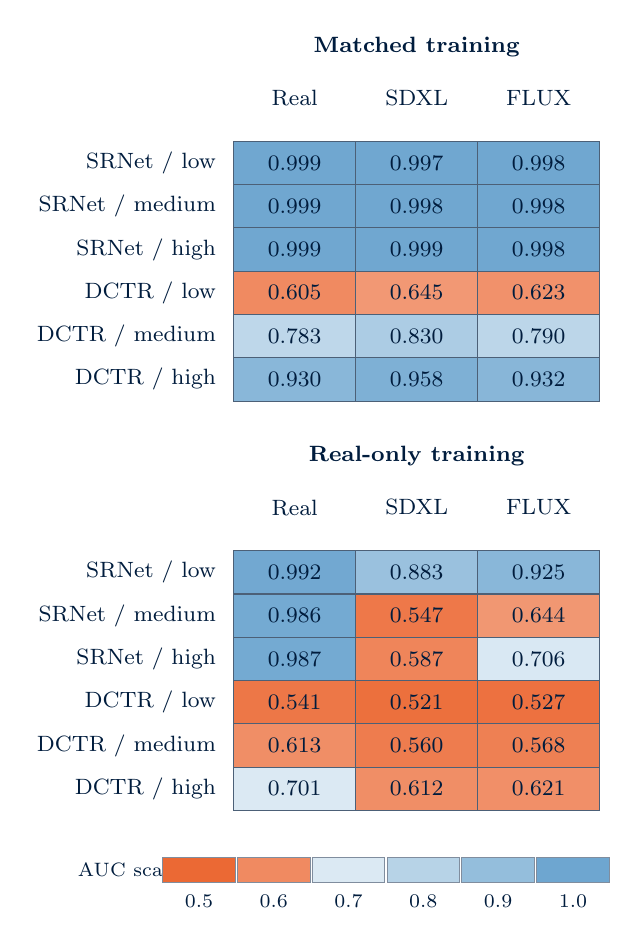
\begin{tikzpicture}[
  cellbase/.style={draw=umdark!70, line width=0.4pt},
]
% Two 6x3 grids stacked vertically so each panel can render at native column width
% without \resizebox shrinking. Rows = (detector x payload), cols = (real, ai_a, ai_b).

\def\cw{1.55}     % cell width  (native, no resizebox)
\def\ch{0.55}     % cell height
\def\rowlbl{2.10} % left margin for row labels
\def\paneldy{5.20} % vertical offset from panel 0 to panel 1 (downward); large enough
                   % for panel-1 title to clear panel-0 bottom row + breathing room

% --- Both panels: titles + column headers (pushed well above cells)
% Cell-grid top of each panel is at \py + 1.65cm (3 rows above midline x \ch = 3*0.55).
% Column header at \py + 2.20cm  (0.55cm above cell top)
% Panel title  at \py + 2.85cm  (0.65cm above header)
\foreach \panel/\panelY/\title in {0/0/{Matched training}, 1/{-\paneldy}/{Real-only training}} {
  \pgfmathsetmacro{\py}{\panelY}
  \node[font=\footnotesize\bfseries\color{umdark}] at (\rowlbl+1.5*\cw, \py+2.85) {\title};
  \foreach \j/\src in {0/Real, 1/SDXL, 2/FLUX} {
    \pgfmathsetmacro{\xx}{\rowlbl+\j*\cw+\cw/2}
    \node[font=\footnotesize\color{umdark}] at (\xx, \py+2.20) {\src};
  }
  \foreach \r/\lbl in {0/{SRNet / low}, 1/{SRNet / medium}, 2/{SRNet / high},
                        3/{DCTR / low}, 4/{DCTR / medium}, 5/{DCTR / high}} {
    \pgfmathsetmacro{\yy}{\py+(2.5-\r)*\ch}
    \node[font=\footnotesize\color{umdark}, anchor=east] at (\rowlbl-0.10, \yy) {\lbl};
  }
}

% --- Cells: \panel, \row, \col, \value. Panel 0 = matched (V1), Panel 1 = real-only (V2a).
\foreach \p/\r/\c/\v in {%
  0/0/0/0.999, 0/0/1/0.997, 0/0/2/0.998,
  0/1/0/0.999, 0/1/1/0.998, 0/1/2/0.998,
  0/2/0/0.999, 0/2/1/0.999, 0/2/2/0.998,
  0/3/0/0.605, 0/3/1/0.645, 0/3/2/0.623,
  0/4/0/0.783, 0/4/1/0.830, 0/4/2/0.790,
  0/5/0/0.930, 0/5/1/0.958, 0/5/2/0.932,
  1/0/0/0.992, 1/0/1/0.883, 1/0/2/0.925,
  1/1/0/0.986, 1/1/1/0.547, 1/1/2/0.644,
  1/2/0/0.987, 1/2/1/0.587, 1/2/2/0.706,
  1/3/0/0.541, 1/3/1/0.521, 1/3/2/0.527,
  1/4/0/0.613, 1/4/1/0.560, 1/4/2/0.568,
  1/5/0/0.701, 1/5/1/0.612, 1/5/2/0.621%
} {
  \pgfmathsetmacro{\panelY}{-\p*\paneldy}
  \pgfmathsetmacro{\xx}{\rowlbl+\c*\cw}
  \pgfmathsetmacro{\yy}{\panelY+(2.5-\r)*\ch-\ch/2}
  \ifdim\v pt<0.70pt
    \pgfmathsetmacro{\fillpct}{int(85-(\v-0.5)*180)}
    \fill[umorange!\fillpct, cellbase] (\xx,\yy) rectangle (\xx+\cw,\yy+\ch);
  \else
    \pgfmathsetmacro{\fillpct}{int(20+(\v-0.7)*200)}
    \fill[umlight!\fillpct, cellbase] (\xx,\yy) rectangle (\xx+\cw,\yy+\ch);
  \fi
  \draw[cellbase] (\xx,\yy) rectangle (\xx+\cw,\yy+\ch);
  \node[font=\footnotesize\color{umdark}, anchor=center] at (\xx+\cw/2,\yy+\ch/2) {\v};
}

% --- Colour-bar legend (below the lower panel)
\begin{scope}[shift={(0, -\paneldy - 2.40)}]
  \node[font=\scriptsize\color{umdark}, anchor=west] at (0.0,0) {AUC scale:};
  \foreach \i/\auc in {0/0.5, 1/0.6, 2/0.7, 3/0.8, 4/0.9, 5/1.0} {
    \pgfmathsetmacro{\xx}{1.20 + \i*0.95}
    \ifdim\auc pt<0.70pt
      \pgfmathsetmacro{\pct}{int(85-(\auc-0.5)*180)}
      \fill[umorange!\pct] (\xx,-0.16) rectangle (\xx+0.92,0.16);
    \else
      \pgfmathsetmacro{\pct}{int(20+(\auc-0.7)*200)}
      \fill[umlight!\pct] (\xx,-0.16) rectangle (\xx+0.92,0.16);
    \fi
    \draw[umdark!50, line width=0.3pt] (\xx,-0.16) rectangle (\xx+0.92,0.16);
    \node[font=\scriptsize\color{umdark}] at (\xx+0.46,-0.40) {\auc};
  }
\end{scope}
\end{tikzpicture}
\caption{Per-(detector, payload, source) test AUC under matched training (top) vs real-only training (bottom). Orange blocks (AUC $\!<\!0.7$) materialise only in the AI columns the real-only model never saw at training time; the real column stays blue throughout.}
\label{fig:matched-vs-realonly-heatmap}
\end{figure}

\begin{figure}[!t]
\centering
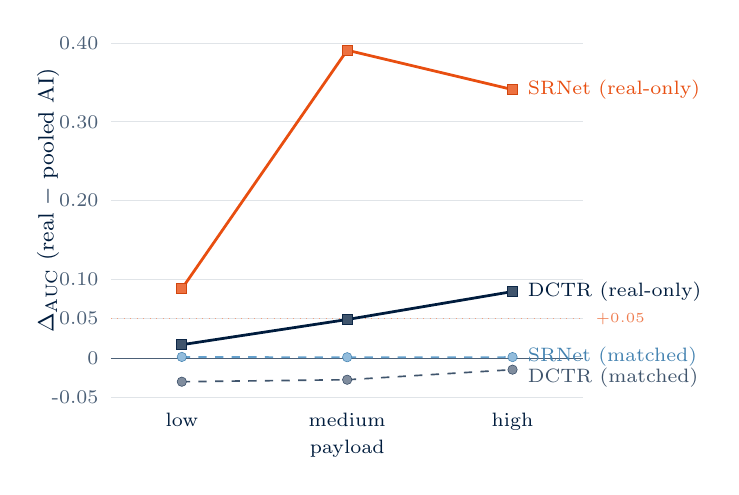
\begin{tikzpicture}[
  v1srnet/.style ={line width=0.6pt, draw=umlight!85, dashed},
  v1dctr/.style  ={line width=0.6pt, draw=umdark!75,  dashed},
  v2srnet/.style ={line width=1.0pt, draw=umorange},
  v2dctr/.style  ={line width=1.0pt, draw=umdark},
  mkV1S/.style ={circle,    draw=umlight!90!black, fill=umlight!60, inner sep=0pt, minimum size=3.4pt, line width=0.2pt},
  mkV1D/.style ={circle,    draw=umdark!80,        fill=umdark!50,  inner sep=0pt, minimum size=3.4pt, line width=0.2pt},
  mkV2S/.style ={rectangle, draw=umorange!90!black, fill=umorange!80, inner sep=0pt, minimum size=3.6pt, line width=0.25pt},
  mkV2D/.style ={rectangle, draw=umdark!95,         fill=umdark!75,   inner sep=0pt, minimum size=3.6pt, line width=0.25pt},
]
\def\xL{0}\def\xR{6.0}
\def\xlow{0.9}\def\xmed{3.0}\def\xhigh{5.1}
% y: Delta in [-0.05, +0.45] -> y = (val + 0.05) * 10
\foreach \v in {-0.05,0,0.05,0.10,0.20,0.30,0.40} {
  \pgfmathsetmacro{\y}{(\v + 0.05) * 10}
  \draw[umdark!12, line width=0.3pt] (\xL,\y) -- (\xR,\y);
  \node[font=\scriptsize\color{umdark!70}, left=1pt] at (\xL,\y) {\v};
}
% zero line
\pgfmathsetmacro{\yzero}{(0+0.05)*10}
\draw[umdark!70, line width=0.4pt] (\xL,\yzero) -- (\xR,\yzero);
% ±0.05 reference (dotted orange)
\pgfmathsetmacro{\yfp}{(0.05+0.05)*10}
\draw[umorange!55, line width=0.35pt, dotted] (\xL,\yfp) -- (\xR,\yfp);
\node[font=\tiny\color{umorange!75}, right=1pt] at (\xR,\yfp) {$+0.05$};
% x labels
\node[font=\scriptsize\color{umdark}, below=2pt] at (\xlow,0)  {low};
\node[font=\scriptsize\color{umdark}, below=2pt] at (\xmed,0)  {medium};
\node[font=\scriptsize\color{umdark}, below=2pt] at (\xhigh,0) {high};
\node[font=\scriptsize\color{umdark}, below=12pt] at (\xmed,0) {payload};
\node[font=\footnotesize\color{umdark}, rotate=90] at (-0.8,2.5) {$\Delta_\text{AUC}$ (real $-$ pooled AI)};
% Lines, drawn back-to-front: V1 first (faded dashed), V2a on top (solid).
% V1 SRNet (LSB-branch, matched): +0.0015, +0.0011, +0.0013 (Table~\ref{tab:learned-headline-auc}, RQ1 deltas)
\pgfmathsetmacro{\yas}{(0.0015+0.05)*10}\pgfmathsetmacro{\ybs}{(0.0011+0.05)*10}\pgfmathsetmacro{\ycs}{(0.0013+0.05)*10}
\draw[v1srnet] (\xlow,\yas) -- (\xmed,\ybs) -- (\xhigh,\ycs);
\node[mkV1S] at (\xlow,\yas){};\node[mkV1S] at (\xmed,\ybs){};\node[mkV1S] at (\xhigh,\ycs){};
% V1 DCTR (DCT-branch, matched): -0.030, -0.028, -0.015
\pgfmathsetmacro{\yad}{(-0.030+0.05)*10}\pgfmathsetmacro{\ybd}{(-0.0275+0.05)*10}\pgfmathsetmacro{\ycd}{(-0.0147+0.05)*10}
\draw[v1dctr] (\xlow,\yad) -- (\xmed,\ybd) -- (\xhigh,\ycd);
\node[mkV1D] at (\xlow,\yad){};\node[mkV1D] at (\xmed,\ybd){};\node[mkV1D] at (\xhigh,\ycd){};
% V2a SRNet (real-only): +0.088, +0.391, +0.341 (Table~\ref{tab:v1-vs-v2a})
\pgfmathsetmacro{\YaS}{(0.088+0.05)*10}\pgfmathsetmacro{\YbS}{(0.391+0.05)*10}\pgfmathsetmacro{\YcS}{(0.341+0.05)*10}
\draw[v2srnet] (\xlow,\YaS) -- (\xmed,\YbS) -- (\xhigh,\YcS);
\node[mkV2S] at (\xlow,\YaS){};\node[mkV2S] at (\xmed,\YbS){};\node[mkV2S] at (\xhigh,\YcS){};
% V2a DCTR (real-only): +0.017, +0.049, +0.0845
\pgfmathsetmacro{\YaD}{(0.017+0.05)*10}\pgfmathsetmacro{\YbD}{(0.049+0.05)*10}\pgfmathsetmacro{\YcD}{(0.0845+0.05)*10}
\draw[v2dctr] (\xlow,\YaD) -- (\xmed,\YbD) -- (\xhigh,\YcD);
\node[mkV2D] at (\xlow,\YaD){};\node[mkV2D] at (\xmed,\YbD){};\node[mkV2D] at (\xhigh,\YcD){};
% End-of-line labels
\node[font=\scriptsize\color{umorange}, right=2pt] at (\xhigh,\YcS) {SRNet (real-only)};
\node[font=\scriptsize\color{umdark}, right=2pt] at (\xhigh,\YcD) {DCTR (real-only)};
\node[font=\scriptsize\color{umlight!90!black}, right=2pt] at (\xhigh,\ycs) {SRNet (matched)};
\node[font=\scriptsize\color{umdark!75}, right=2pt] at (\xhigh,\ycd-0.1) {DCTR (matched)};
\end{tikzpicture}
\caption{Learned-detector payload trend, parallel to Fig.~\ref{fig:rq3}. Matched-training detectors (dashed, light markers) sit near zero, SRNet at ceiling, DCTR slightly real-harder. Real-only training (solid, square markers) flips direction and inflates the gap by $5$--$300\times$: SRNet peaks at medium payload (real-easier by $+0.39$~AUC), DCTR grows monotonically with payload.}
\label{fig:learned-payload-trend}
\end{figure}

\begin{table}[!htbp]
\centering\footnotesize
\caption{Real-only training: held-out-of-training-corpus AUC (``Val'') and per-source test-corpus AUC at the plain-encryption cell. DCTR also carries an $E_\text{OOB}$ ensemble residual (see Fig.~\ref{fig:dctr-eoob-ladder}).}
\label{tab:v2a-results}
\setlength{\tabcolsep}{4pt}\renewcommand{\arraystretch}{1.05}
\begin{tabular}{@{}llccccc@{}}
\toprule
\textbf{Det.} & \textbf{Payload} & \textbf{Val} & \textbf{$E_\text{OOB}$} & \textbf{Real} & \textbf{AI-A} & \textbf{AI-B} \\
\midrule
SRNet & low    & 1.0000 & --       & 0.992 & 0.883 & 0.925 \\
SRNet & medium & 1.0000 & --       & 0.986 & 0.547 & 0.644 \\
SRNet & high   & 1.0000 & --       & 0.988 & 0.587 & 0.706 \\
DCTR  & low    & 0.6329 & 0.4563   & 0.541 & 0.521 & 0.527 \\
DCTR  & medium & 0.8306 & 0.2570   & 0.613 & 0.560 & 0.568 \\
DCTR  & high   & 0.9562 & 0.1012   & 0.701 & 0.612 & 0.621 \\
\bottomrule
\end{tabular}
\end{table}

\begin{table}[!htbp]
\centering\footnotesize
\caption{Matched vs.\ real-only training: per-source test AUC at the plain-encryption cell. Bold marks drops $\geq 0.10$ from matched $\to$ real-only, the training-balance signature.}
\label{tab:v1-vs-v2a}
\setlength{\tabcolsep}{3pt}\renewcommand{\arraystretch}{1.05}
\begin{tabular}{@{}ll | ccc | ccc@{}}
\toprule
& & \multicolumn{3}{c}{\textbf{matched training}} & \multicolumn{3}{c}{\textbf{real-only training}} \\
\textbf{Det.} & \textbf{Payload} & Real & AI-A & AI-B & Real & AI-A & AI-B \\
\midrule
SRNet & low    & 0.999 & 0.997 & 0.998 & 0.992 & \textbf{0.883} & \textbf{0.925} \\
SRNet & medium & 0.999 & 0.998 & 0.998 & 0.986 & \textbf{0.547} & \textbf{0.644} \\
SRNet & high   & 0.999 & 0.999 & 0.998 & 0.988 & \textbf{0.587} & \textbf{0.706} \\
DCTR  & low    & 0.605 & 0.645 & 0.623 & 0.541 & 0.521 & 0.527 \\
DCTR  & medium & 0.783 & 0.830 & 0.790 & 0.613 & \textbf{0.560} & \textbf{0.568} \\
DCTR  & high   & 0.930 & 0.958 & 0.932 & 0.701 & \textbf{0.612} & \textbf{0.621} \\
\bottomrule
\end{tabular}
\end{table}

\paragraph{Verdict from the matched-vs-real-only contrast: training-balance artefact, decisively.} Real-only-trained SRNet retains near-perfect detection on the carrier source it was trained on (real, AUC 0.99 across all three payload levels) but \emph{collapses on the unseen AI sources}, dropping to AUC 0.55--0.71 on AI-A (SDXL) and 0.64--0.93 on AI-B (FLUX), a $0.26$--$0.45$~AUC gap relative to its same-payload performance on real photographs.  The matched-training SRNet per-source flatness (range $\sim$0.003 at every cell, Table~\ref{tab:v1-vs-v2a}) is therefore \emph{not} architectural source-invariance: it is a consequence of training on a 1:1:1 carrier mix that included the test-time AI sources. When the training mix is removed, the deep spatial CNN reveals a substantial real-vs-AI generalisation gap consistent with the cover-source-mismatch literature~\cite{giboulot2020csm,mallet2024csm,mereur2024deepfake}. DCTR shows the same pattern at smaller absolute magnitude: the matched-training small AI-easier ordering (ai\_a $>$ real by 0.02--0.04) flips under real-only training to real-easier (real $>$ ai\_a/ai\_b by 0.02--0.09) and overall AUC drops on every cell, confirming that the matched-training DCTR per-source pattern was also a training-balance artefact rather than an intrinsic feature of the DCTR feature set. (Both training configurations use a single seed (\texttt{4242}); see Section~\ref{sec:limitations} for the single-seed and Flickr-only-vs-mixed-test-corpus caveats.)

\begin{figure}[!t]
\centering
\resizebox{\columnwidth}{!}{%
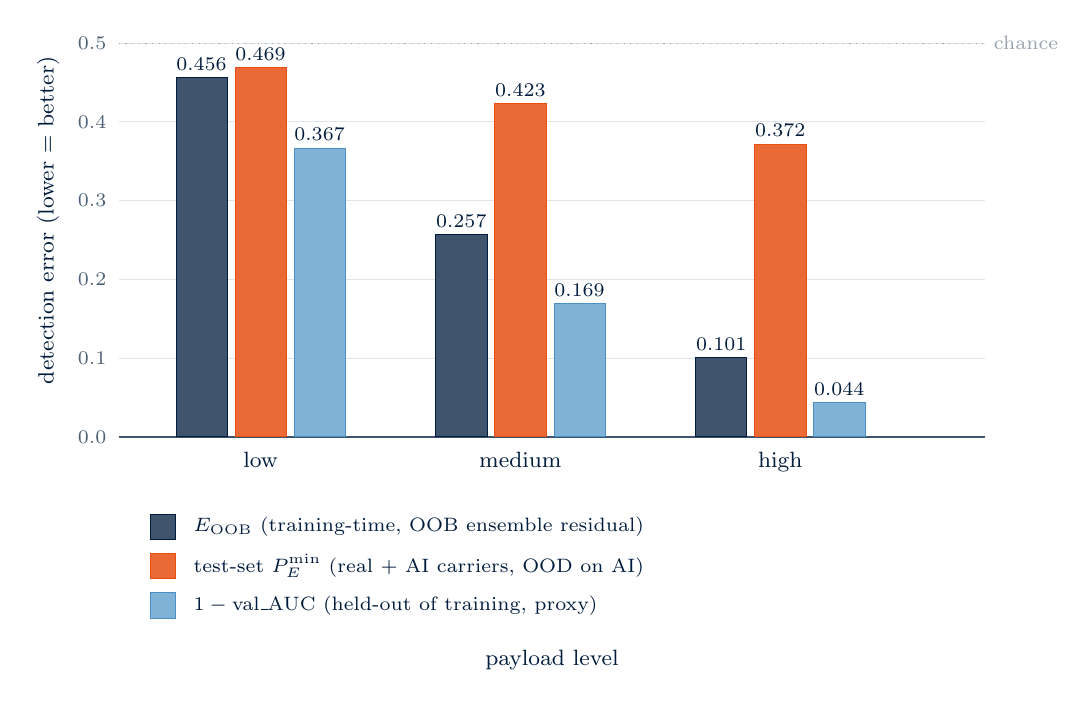
\begin{tikzpicture}[
  barEoob/.style ={draw=umdark,  fill=umdark!75,  line width=0.25pt},
  barTest/.style ={draw=umorange,fill=umorange!85,line width=0.25pt},
  barVal/.style  ={draw=umlight, fill=umlight!70, line width=0.25pt},
]
% y-axis: detection error in [0, 0.55] -> [0, 5.5 cm]; chance at 0.5 -> 5 cm
\foreach \v in {0.0,0.1,0.2,0.3,0.4,0.5} {
  \pgfmathsetmacro{\y}{\v * 10}
  \draw[umdark!12, line width=0.3pt] (0,\y) -- (11.0,\y);
  \node[font=\scriptsize\color{umdark!70}, left=1pt] at (0,\y) {\v};
}
% chance line at 0.5
\draw[umdark!40, line width=0.4pt, dotted] (0,5) -- (11.0,5)
  node[font=\scriptsize\color{umdark!70}, right=2pt, fill=white, inner sep=1pt] {chance};
\draw[umdark!75, line width=0.5pt] (0,0) -- (11.0,0);
\node[font=\footnotesize\color{umdark}, rotate=90] at (-0.9,2.75) {detection error (lower = better)};

\def\bw{0.65}
\def\bg{0.10}
\foreach \i/\name/\eoob/\test/\val in {%
  0/low/0.456/0.469/0.367,
  1/medium/0.257/0.423/0.169,
  2/high/0.101/0.372/0.044%
} {
  \pgfmathsetmacro{\xc}{1.8 + \i*3.30}
  \pgfmathsetmacro{\xa}{\xc - 1.5*\bw - \bg}
  \pgfmathsetmacro{\xb}{\xc - 0.5*\bw}
  \pgfmathsetmacro{\xcc}{\xc + 0.5*\bw + \bg}
  \pgfmathsetmacro{\heo}{\eoob * 10}
  \pgfmathsetmacro{\hte}{\test * 10}
  \pgfmathsetmacro{\hva}{\val  * 10}
  \draw[barEoob] (\xa,0)  rectangle (\xa+\bw,\heo);
  \draw[barTest] (\xb,0)  rectangle (\xb+\bw,\hte);
  \draw[barVal]  (\xcc,0) rectangle (\xcc+\bw,\hva);
  \node[font=\scriptsize\color{umdark}, above=-1pt] at (\xa+\bw/2, \heo) {\eoob};
  \node[font=\scriptsize\color{umdark}, above=-1pt] at (\xb+\bw/2, \hte) {\test};
  \node[font=\scriptsize\color{umdark}, above=-1pt] at (\xcc+\bw/2,\hva) {\val};
  \node[font=\footnotesize\color{umdark}, below=2pt] at (\xc,0) {\name};
}
% Legend below the bars
\begin{scope}[shift={(0.4, -1.3)}]
  \draw[barEoob] (0,0) rectangle (0.32,0.32);
  \node[font=\scriptsize\color{umdark}, right=3pt] at (0.32,0.16) {$E_\mathrm{OOB}$ (training-time, OOB ensemble residual)};
  \draw[barTest] (0,-0.5) rectangle (0.32,-0.18);
  \node[font=\scriptsize\color{umdark}, right=3pt] at (0.32,-0.34) {test-set $P_E^{\min}$ (real + AI carriers, OOD on AI)};
  \draw[barVal]  (0,-1.0) rectangle (0.32,-0.68);
  \node[font=\scriptsize\color{umdark}, right=3pt] at (0.32,-0.84) {$1-\mathrm{val\_AUC}$ (held-out of training, proxy)};
\end{scope}
\node[font=\footnotesize\color{umdark}, below=8pt] at (5.5,-2.3) {payload level};
\end{tikzpicture}}
\caption{DCTR under real-only training: training-time $E_\mathrm{OOB}$ (dark), in-distribution validation proxy $1\!-\!\mathrm{val\_AUC}$ (light), and operational test-set $P_E^{\min}$ on a real$+$AI corpus (orange). The gap between dark and orange is the cover-source-mismatch effect at the operational metric.}
\label{fig:dctr-eoob-ladder}
\end{figure}

\begin{figure}[!t]
\centering
\resizebox{\columnwidth}{!}{%
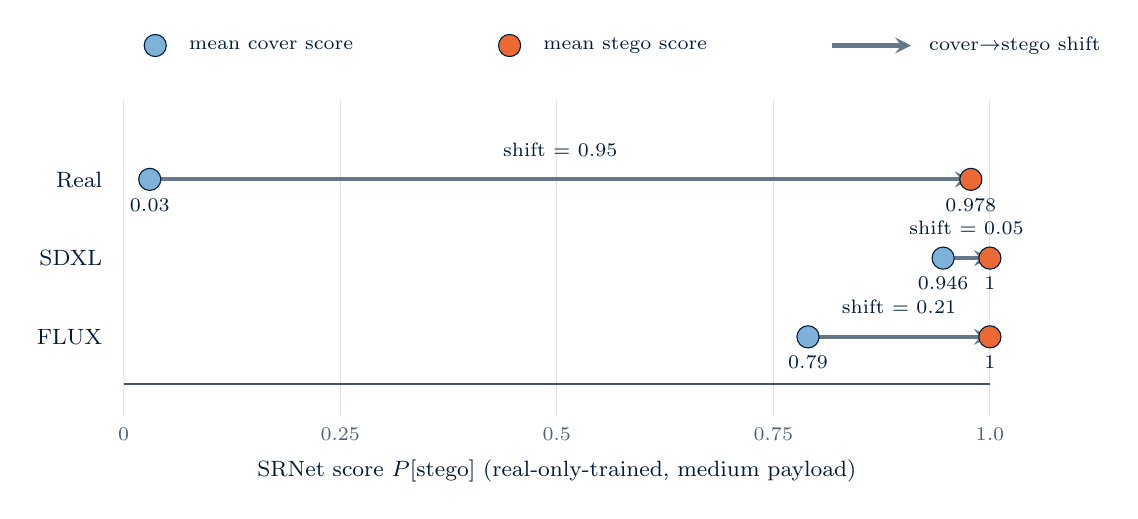
\begin{tikzpicture}[
  covermk/.style={circle, draw=umdark, fill=umlight!70, line width=0.4pt, minimum size=8pt, inner sep=0pt},
  stegomk/.style={circle, draw=umdark, fill=umorange!85, line width=0.4pt, minimum size=8pt, inner sep=0pt},
  shiftarr/.style={->, >=stealth, line width=1.5pt, draw=umdark!60},
]
% Three rows: real (top), SDXL (middle), FLUX (bottom).
% Per row, plot the cover-mean (blue circle) and stego-mean (orange circle) on a [0,1] axis,
% with an arrow connecting them showing the "shift" (which collapses on AI carriers).

% X-axis: 0 -> 0 cm, 1 -> 11 cm
\foreach \v in {0,0.25,0.5,0.75,1.0} {
  \pgfmathsetmacro{\x}{\v * 11}
  \draw[umdark!12, line width=0.3pt] (\x,-0.4) -- (\x,3.6);
  \node[font=\scriptsize\color{umdark!70}, below=1pt] at (\x,-0.4) {\v};
}
\node[font=\footnotesize\color{umdark}] at (5.5,-1.1) {SRNet score $P[\mathrm{stego}]$ (real-only-trained, medium payload)};
\draw[umdark!75, line width=0.5pt] (0,0) -- (11,0);

% Per-source rows
\foreach \i/\src/\cover/\stego in {%
  0/{FLUX}/0.790/1.000,
  1/{SDXL}/0.946/1.000,
  2/{Real}/0.030/0.978%
} {
  \pgfmathsetmacro{\yy}{0.6 + \i*1.0}
  \pgfmathsetmacro{\xc}{\cover*11}
  \pgfmathsetmacro{\xs}{\stego*11}
  \pgfmathsetmacro{\shift}{\stego-\cover}
  \node[font=\footnotesize\color{umdark}, anchor=east] at (-0.15, \yy) {\src};
  \draw[shiftarr] (\xc,\yy) -- (\xs,\yy);
  \node[covermk] at (\xc,\yy) {};
  \node[stegomk] at (\xs,\yy) {};
  \node[font=\scriptsize\color{umdark}, above=2pt] at ({(\xc+\xs)/2}, \yy+0.1) {shift = \pgfmathprintnumber[fixed,precision=2]{\shift}};
  % Per-marker value
  \node[font=\scriptsize\color{umdark}, below=2pt] at (\xc,\yy-0.05) {\pgfmathprintnumber[fixed,precision=3]{\cover}};
  \node[font=\scriptsize\color{umdark}, below=2pt] at (\xs,\yy-0.05) {\pgfmathprintnumber[fixed,precision=3]{\stego}};
}

% Legend
\begin{scope}[shift={(0.4, 4.3)}]
  \node[covermk] at (0,0) {};
  \node[font=\scriptsize\color{umdark}, right=3pt] at (0.2,0) {mean cover score};
  \node[stegomk] at (4.5,0) {};
  \node[font=\scriptsize\color{umdark}, right=3pt] at (4.7,0) {mean stego score};
  \draw[shiftarr] (8.6,0) -- (9.6,0);
  \node[font=\scriptsize\color{umdark}, right=3pt] at (9.6,0) {cover$\to$stego shift};
\end{scope}
\end{tikzpicture}}
\caption{Real-only-trained SRNet, medium payload: cover- and stego-mean scores per carrier source; the arrow is the cover-to-stego shift. On real carriers separation is clean (shift 0.95); on AI carriers diffusion noise pushes covers into the stego region and separation collapses to 0.05 (SDXL) / 0.21 (FLUX).}
\label{fig:v2a-srnet-mechanism}
\end{figure}

\paragraph{Implication for RQ1.} Re-running the cross-validation pipeline on the real-only predictions flips four of the five RQ verdicts at the learned-detector family level: RQ1 from trivial ($\Delta\!=\!+0.0012$) to supported with $\Delta\!=\!+0.2473$ (CI $[+0.245,+0.250]$); RQ2 from trivial to supported with $\Delta\!=\!-0.0689$; RQ4 (spatial vs.\ frequency branch contrast) from trivial to supported with $\Delta\!=\!+0.2195$; RQ3 retains the mixed verdict but the per-payload real-minus-AI gaps grow from $\{-0.014, -0.013, -0.007\}$ to $\{+0.053, +0.220, +0.213\}$. RQ5 (encryption invariance) is unchanged at $\Delta\!\approx\!0$ as expected, an encryption ablation does not depend on training-set carrier composition.

\paragraph{Mechanism of the real-only medium/high-payload collapse on AI carriers.} The per-(payload, source, label) SRNet score decomposition (Fig.~\ref{fig:v2a-srnet-mechanism}) shows the failure mode directly: at medium and high payload, real-only-trained SRNet assigns AI \emph{covers} a near-saturated stego score (0.79--0.95) almost indistinguishable from the score on AI \emph{stegos} (1.000); the cover-stego shift on AI carriers collapses to $0.05$--$0.27$ (vs.\ $0.95$ on real). The medium checkpoint was trained to separate ``real cover'' from ``real cover $+$ 15\,\% LSB perturbation,'' and at test time it interprets AI covers' diffusion-decoder noise patterns as the perturbation it was trained to detect. The effect is weaker at high payload and largely absent at low payload, where the tighter decision boundary still admits separation. Structurally this matches the cover-side variance-inflation mechanism we identify for $\chi^2$-spatial in Section~\ref{sec:chi2spatial}, both detectors register diffusion-decoder noise as a stego-like signal on the cover side.

\subsection{Strongest-Detector Comparison}

The best-vs-best AUC (learned vs.\ strongest same-branch classical detector, averaged over encryption) reveals a branch-asymmetric picture: in the \textbf{LSB branch} SRNet beats sample\_pairs by $\{+0.065, +0.010, +0.001\}$ at \{low, medium, high\} payload (advantage shrinks as the classical detector approaches the ceiling); in the \textbf{DCT branch} our tile-local $\chi^2$-DCT-tiled variant (Section~\ref{sec:tiled}) outperforms DCTR by $\{+0.047, +0.109, +0.058\}$ across the same payload cells. The takeaway for detector selection: a deep spatial CNN is the right tool for LSB, but frequency-domain steganalysis remains a regime where a well-designed classical detector still dominates.

\paragraph{Provenance.} The training-set caption manifests (matched and real-only), model checkpoints, per-cell training logs, and the leakage-guard SHA-256 hashes are included in the supplementary deliverables bundle. The classical-detector predictions, the matched- and real-only-trained learned-detector predictions, and the verdict tables in this section are all reproducible from the manifests $+$ the seed (\texttt{4242}).

% ============================================================
\section{Detector-Level Contributions}
\label{sec:detector-side}
% ============================================================

The five RQs and the cross-validation evaluate the carrier-source effect using detectors that we treat as fixed instruments.  Two by-products of that evaluation are themselves contributions to the steganalysis literature, independent of the carrier-source question: a tile-local variant of the Westfeld pairs-of-values test that out-performs every classical DCT detector in our pipeline (\S\ref{sec:tiled}), and a candidate mechanism for why the $\chi^2$-spatial detector inverts the carrier-source ordering reported by every other detector in our suite (an inversion that is operationally negligible under pAUC; \S\ref{sec:chi2spatial}).

% ----------------------------------------------------------------
\subsection{Tile-Local $\chi^2$-DCT Detector}
\label{sec:tiled}
% ----------------------------------------------------------------

The strongest frequency-branch detector in our pipeline is not the textbook global Westfeld $\chi^2$-DCT but a \textbf{tile-local variant} we introduce. The image's $8\!\times\!8$ DCT-block grid is partitioned into a coarse $T\!\times\!T$ grid of disjoint tiles ($T\!=\!2$ in our runs, giving four tiles); the Westfeld pairs-of-values $\chi^2$ statistic is computed independently within each tile's non-zero AC coefficients, and the \textbf{maximum} per-tile $-\chi^2/(df\!-\!1)$ is returned as the image-level score.

Overall (pooled-payload) AUC is \textbf{0.855}, well above the global $\chi^2$-DCT at 0.756 and behind only the strongest spatial-branch detectors RS (0.967) and sample-pairs (0.973). Figure~\ref{fig:tiled} shows the per-stratum AUC and the ROC curve at medium payload, where the difference between the global and tiled variants is most visible.

\begin{figure}[t]
\centering
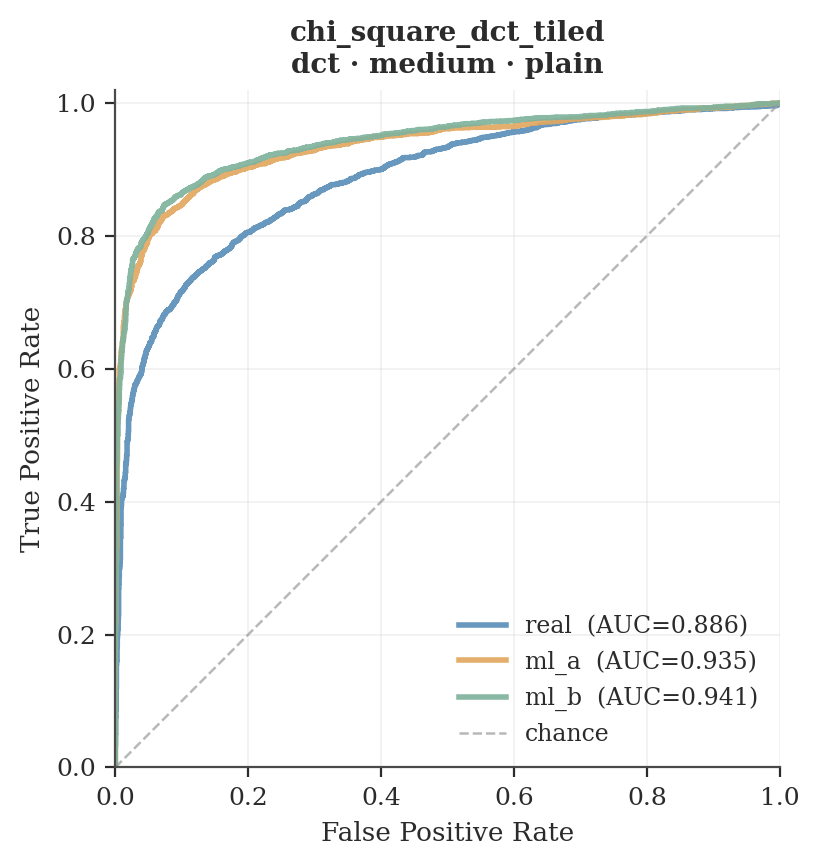
\includegraphics[width=0.86\linewidth]{figures/roc_chi_dct_tiled_med.png}
\caption{ROC curves for $\chi^2$-DCT-tiled at DCT/medium/plain ($N\!=\!3{,}000$). The per-source ordering real (AUC=0.886) $<$ SDXL (0.935) $<$ FLUX (0.941) is consistent with RQ1. The global $\chi^2$-DCT detector on the same data reaches only AUC=0.778, well below the tiled variant.}
\label{fig:tiled}
\end{figure}

\begin{table}[t]
\centering\small
\caption{$\chi^2$-DCT-tiled vs.\ global $\chi^2$-DCT, per (source, payload). Each cell is the per-stratum ROC~AUC; the tiled variant beats the global detector in every cell.}
\label{tab:tiled}
\setlength{\tabcolsep}{4pt}\renewcommand{\arraystretch}{1.1}
\begin{tabular}{@{}l c c c c c c@{}}
\toprule
& \multicolumn{3}{c}{\textbf{$\chi^2$-DCT (global)}} & \multicolumn{3}{c}{\textbf{$\chi^2$-DCT-tiled (ours)}} \\
\cmidrule(lr){2-4}\cmidrule(lr){5-7}
\textbf{Payload} & real & ai\_a & ai\_b & real & ai\_a & ai\_b \\
\midrule
low    & 0.581 & 0.620 & 0.605 & 0.635 & 0.703 & 0.724 \\
medium & 0.727 & 0.806 & 0.775 & 0.886 & 0.936 & 0.941 \\
high   & 0.893 & 0.960 & 0.935 & 0.993 & 0.997 & 0.998 \\
\bottomrule
\end{tabular}
\end{table}

\paragraph{Why does tiling help?} DCT statistics are not spatially uniform across either photographic or diffusion carriers. Textured regions and smooth regions produce very different per-block pairs-of-values histograms. The global detector mixes all blocks into one histogram, which has two effects on the test statistic: (1)~the central-limit averaging hides any localised stego signal, and (2)~the carrier's natural inter-region heterogeneity inflates the cover-side $\chi^2$ noise floor. Tiling separates these regions before applying the test, and max-pooling exposes the tile with the strongest stego-like evidence. The mechanism is the same as Westfeld and Pfitzmann's original sliding-window suggestion~\cite{westfeld1999chi} for detecting \emph{sequential} embedding, but our tiles are coarser and disjoint, which keeps tile-level $\chi^2$ counts large enough to be stable.

\paragraph{Literature support.} Local chi-square variants appear in several places. Westfeld and Pfitzmann themselves discuss a sliding-window form for sequential payloads~\cite{westfeld1999chi}; Provos's outguess paper~\cite{provos2001outguess} notes that the global PoV test loses power as embedding becomes more local; the broader steganalysis literature on \emph{block-wise} or \emph{regional} features (e.g.\ rich-model and DCTR-style approaches~\cite{fridrich2012srm,holub2015dctr}) is essentially built on the same insight at a finer granularity. The tile-local Westfeld $\chi^2$ as we implement it, a coarse $2\!\times\!2$ disjoint partition with max-pooling, returning the underflow-free $-\chi^2/df$ score, is a simple and, to our knowledge, under-tested combination of those ingredients.

\paragraph{Caveats.} Two properties of the within-corpus result remain after the BOSSBase validation below.  \textit{(i)}~Max-pooling raises false-positive risk: the detector's score on a cover image is the noisiest of $T^2$ $\chi^2$ samples, which can exceed the global $\chi^2$ on the same image.  Paired-AUC controls for this in the within-corpus contrast but a deployed setting would need explicit recalibration against natural-image false-positive rates.  \textit{(ii)}~Adaptive (DCT-domain content-driven) embeddings such as J-UNIWARD~\cite{holub2014uniward} and the histogram-preserving OutGuess~\cite{provos2001outguess} (see Section~\ref{sec:tiled-validation}) lie outside the scope of a pairs-of-values test by construction; the result is bounded to non-adaptive DCT-LSB-style embedders.

\paragraph{Validation on BOSSBase.}
\label{sec:tiled-validation}
To probe whether the gain transfers off the caption-matched corpus, the detector was re-evaluated on BOSSBase~1.01~\cite{bas2011boss} (10{,}000 covers, 120{,}000 stegos at six bpnzAC payloads $\times$ two encryption modes), at both Q$=$75 and Q$=$95 and against two non-adaptive DCT-LSB embedders, JSteg and OutGuess~\cite{provos2001outguess}.  Mean AUC and mean $P_E^{\min}$ over the 12 (payload$\times$encryption) cells per (Q, embedder, detector) are reported in Table~\ref{tab:bossbase-tile-local}.  On JSteg the tile-local detector beats the global $\chi^2$ by $+0.086$--$0.090$~AUC at both quality factors, with $P_E^{\min}$ dropping from $\sim 0.24$--$0.29$ to $\sim 0.13$--$0.19$: the within-corpus gain reproduces on the canonical benchmark.  On OutGuess all three $\chi^2$-DCT variants collapse to AUC~$\approx 0.50$ as expected from the histogram-preservation property; the sliding-window $\chi^2$ retains a small ($\sim 0.58$~AUC) residual signal, plausibly because OutGuess's random correction path leaves a non-uniform residual at the window scale, but this is not operationally useful.  The BOSSBase $T$-sweep over $T\!\in\!\{1,2,3,4,6,8\}$ (collapsed across the 12 payload$\times$encryption cells, JSteg, max-pool) shows the AUC continues to climb past our caption-matched-corpus choice of $T\!=\!2$: at Q$=$75 the per-$T$ AUCs are $\{0.76, 0.85, 0.89, 0.90, 0.90, 0.85\}$ (peak $T\!=\!4$); at Q$=$95, $\{0.82, 0.90, 0.93, 0.95, 0.97, 0.95\}$ (peak $T\!=\!6$). The $T\!=\!2$ headline configuration is therefore conservative on BOSSBase; the optimum drifts to $T\!\approx\!4$--$6$, and a future-work cross-payload $T$-sweep on the caption-matched corpus would test whether the same drift holds on diffusion carriers.

\begin{table}[!t]
\centering\footnotesize
\caption{BOSSBase~1.01: mean AUC and $P_E^{\min}$ over 12 (payload$\times$encryption) cells per (Q, embedder, detector). Bold marks tile-local beating global $\chi^2$ on JSteg by $0.086$--$0.090$~AUC; both at chance on the histogram-preserving OutGuess.}
\label{tab:bossbase-tile-local}
\begin{tabular}{llcccc}
\toprule
 & & \multicolumn{2}{c}{AUC} & \multicolumn{2}{c}{$P_E^{\min}$} \\
\cmidrule(lr){3-4}\cmidrule(lr){5-6}
Q & embedder & global & tile-local & global & tile-local \\
\midrule
75 & JSteg    & 0.764 & \textbf{0.854} & 0.286 & \textbf{0.192} \\
95 & JSteg    & 0.816 & \textbf{0.902} & 0.237 & \textbf{0.134} \\
75 & OutGuess & 0.502 & 0.500 & 0.498 & 0.496 \\
95 & OutGuess & 0.507 & 0.507 & 0.494 & 0.493 \\
\bottomrule
\end{tabular}
\end{table}

% ----------------------------------------------------------------
\subsection{The $\chi^2$-Spatial Reversal}
\label{sec:chi2spatial}
% ----------------------------------------------------------------

The single detector that reverses the RQ1 direction is the spatial Westfeld $\chi^2$. At medium and high payload, real photographs are easier to attack than diffusion generated carriers by 0.027--0.034~AUC, both Holm-significant. The reversal is robust to the $3\!\times\!$ sample size and persists across both SDXL and FLUX.

\paragraph{Mechanism, direct test.} The Westfeld $\chi^2$ test asks how far the cover's $(2k,\,2k\!+\!1)$ pixel-bit pair counts deviate from equality. To probe the mechanism we ran a falsifying cover-only test: on all 9{,}000 cover images we computed the PoV imbalance
\begin{equation}
S(c) = \sum_{k=0}^{127} |n_{2k}(c) - n_{2k+1}(c)|
\label{eq:pov-imbalance}
\end{equation}
\noindent and the cover-side chi-square score (per-source distribution in Appendix~\ref{app:pov}).

The result \emph{falsifies} the naive ``smoother diffusion outputs $\Rightarrow$ lower cover-side $\chi^2_\text{stat}$'' story. The data show the opposite: AI covers have \emph{slightly higher} PoV imbalance than real photographs (medians: real 9{,}698, ai\_a 10{,}272, ai\_b 11{,}649; paired Wilcoxon $p\!<\!10^{-9}$ both directions). The cover-side chi-square score is also more negative (i.e.\ more imbalanced) on AI carriers (medians: real $-4.03$, ai\_a $-4.93$, ai\_b $-6.27$). Diffusion outputs are not more balanced in this sense.

\paragraph{Mechanism, corrected.} What \emph{does} reverse the AUC is the cover-side score \emph{variance}, not the mean. Cover-side $\chi^2$-spatial score standard deviations are 37.5 (real), 54.4 (ai\_a), 43.0 (ai\_b). At high payload the median cover$\to$stego score shift is in fact \textbf{larger} on ai\_b ($+2.97$) than on real ($+1.95$), but the cover distribution on AI carriers is so much wider that the Cohen's $d$ of cover-vs-stego separation drops from $d\!=\!0.26$ (real) to $d\!=\!0.21$ (ai\_a) and $d\!=\!0.22$ (ai\_b). Interpretation: diffusion outputs have a more \emph{heterogeneous} histogram distribution, some images are very flat, others very textured, producing a wider cover-side score distribution that overlaps more with the stego-side distribution, dropping AUC.

% Fig 16 (PoV box plot) MOVED to appendix; data summary already in prose above + Table~\ref{tab:appendix-pov}.
\iffalse
\begin{figure}[t]
\centering
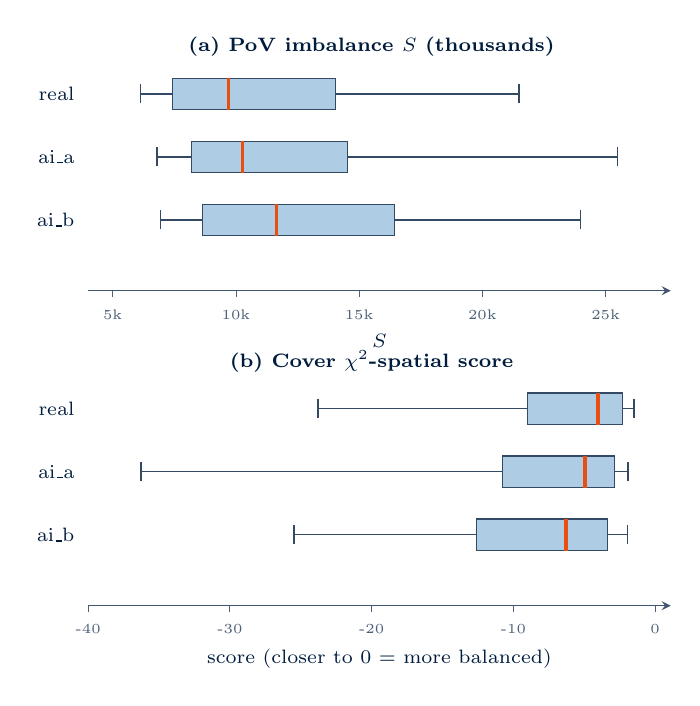
\begin{tikzpicture}[
  whisker/.style={line width=0.5pt, draw=umdark!80},
  box/.style={draw=umdark!80, fill=umlight!45, line width=0.4pt},
  medline/.style={line width=1.2pt, draw=umorange},
  axis/.style={->, >=stealth, umdark!75, line width=0.45pt},
]
% ---------- Panel A: PoV imbalance S (working in kilo-units: divide by 1000 first) ----------
\begin{scope}[shift={(0,0)}]
\node[font=\scriptsize\bfseries\color{umdark}] at (3.6,3.0) {(a) PoV imbalance $S$ (thousands)};
% x-axis: S/1000 in [4, 27], width 7.2 cm, multiplier = 7.2/23 = 0.313
\draw[axis] (0,-0.1) -- (7.4,-0.1);
\foreach \v/\lbl in {5/5k, 10/10k, 15/15k, 20/20k, 25/25k} {
  \pgfmathsetmacro{\x}{(\v-4)*0.313}
  \draw[umdark!70, line width=0.3pt] (\x,-0.1) -- (\x,-0.18);
  \node[font=\tiny\color{umdark!70}, below=1pt] at (\x,-0.18) {\lbl};
}
\node[font=\scriptsize\color{umdark}, below=10pt] at (3.7,-0.18) {$S$};
% per-source rows (S values in thousands)
\foreach \name/\yc/\pa/\qa/\meda/\qb/\pb in {%
  {real}/2.4/6.13/7.42/9.70/14.05/21.49,
  {ai\_a}/1.6/6.79/8.18/10.27/14.52/25.48,
  {ai\_b}/0.8/6.93/8.64/11.65/16.42/23.97%
} {
  \pgfmathsetmacro{\xpa}{(\pa-4)*0.313}
  \pgfmathsetmacro{\xqa}{(\qa-4)*0.313}
  \pgfmathsetmacro{\xmed}{(\meda-4)*0.313}
  \pgfmathsetmacro{\xqb}{(\qb-4)*0.313}
  \pgfmathsetmacro{\xpb}{(\pb-4)*0.313}
  \draw[whisker] (\xpa,\yc) -- (\xpb,\yc);
  \draw[whisker] (\xpa,\yc-0.12) -- (\xpa,\yc+0.12);
  \draw[whisker] (\xpb,\yc-0.12) -- (\xpb,\yc+0.12);
  \draw[box] (\xqa,\yc-0.20) rectangle (\xqb,\yc+0.20);
  \draw[medline] (\xmed,\yc-0.20) -- (\xmed,\yc+0.20);
  \node[font=\scriptsize\color{umdark}, anchor=east] at (-0.05,\yc) {\name};
}
\end{scope}

% ---------- Panel B: cover chi-square score ----------
\begin{scope}[shift={(0,-4.0)}]
\node[font=\scriptsize\bfseries\color{umdark}] at (3.6,3.0) {(b) Cover $\chi^2$-spatial score};
% x-axis: score in [-40, 0], width 7.2 cm, multiplier 7.2/40 = 0.18
\draw[axis] (0,-0.1) -- (7.4,-0.1);
\foreach \v in {-40,-30,-20,-10,0} {
  \pgfmathsetmacro{\x}{(\v+40)*0.18}
  \draw[umdark!70, line width=0.3pt] (\x,-0.1) -- (\x,-0.18);
  \node[font=\tiny\color{umdark!70}, below=1pt] at (\x,-0.18) {\v};
}
\node[font=\scriptsize\color{umdark}, below=10pt] at (3.7,-0.18) {score (closer to 0 = more balanced)};
\foreach \name/\yc/\pa/\qa/\meda/\qb/\pb in {%
  {real}/2.4/-23.78/-9.00/-4.03/-2.27/-1.47,
  {ai\_a}/1.6/-36.27/-10.75/-4.93/-2.87/-1.91,
  {ai\_b}/0.8/-25.48/-12.58/-6.27/-3.36/-1.96%
} {
  \pgfmathsetmacro{\xpa}{(\pa+40)*0.18}
  \pgfmathsetmacro{\xqa}{(\qa+40)*0.18}
  \pgfmathsetmacro{\xmed}{(\meda+40)*0.18}
  \pgfmathsetmacro{\xqb}{(\qb+40)*0.18}
  \pgfmathsetmacro{\xpb}{(\pb+40)*0.18}
  \draw[whisker] (\xpa,\yc) -- (\xpb,\yc);
  \draw[whisker] (\xpa,\yc-0.12) -- (\xpa,\yc+0.12);
  \draw[whisker] (\xpb,\yc-0.12) -- (\xpb,\yc+0.12);
  \draw[box] (\xqa,\yc-0.20) rectangle (\xqb,\yc+0.20);
  \draw[medline] (\xmed,\yc-0.20) -- (\xmed,\yc+0.20);
  \node[font=\scriptsize\color{umdark}, anchor=east] at (-0.05,\yc) {\name};
}
\end{scope}
\end{tikzpicture}
\caption{Cover-only diagnostic for the $\chi^2$-spatial reversal ($n\!=\!3{,}000$ per source). Box = Q1--Q3, whisker = p10--p90, orange line = median. Panel (a): PoV imbalance $S$ from Eq.~\ref{eq:pov-imbalance}; the naive hypothesis predicted AI\,$<$\,real, but real has the \emph{lowest} median (Wilcoxon $p\!<\!10^{-9}$). Panel (b): cover-side $\chi^2$-spatial score; medians track $S$, but the AI distributions are visibly wider (real std 37.5, ai\_a 54.4, ai\_b 43.0). The wider cover-side score distribution is what overwhelms the per-image stego shift and drops the AUC.}
\label{fig:pov}
\end{figure}
\fi

\paragraph{Why other detectors are unaffected.} RS analysis and Sample Pairs do not test pair-of-values balance directly; they reason about local pixel-group regularity (RS) or adjacent-pair multiset statistics (SPA). Neither is dominated by the marginal histogram, so the diffusion-decoder heterogeneity does not flip their direction. The DCT-branch detectors operate in frequency space, where diffusion outputs have if anything \emph{more} histogram structure than photographs (due to the JPEG re-encode step), and there the AI-easier direction holds with the largest practical-significance effects.

\paragraph{Where the reversal lives.} Crucially, the reversal is a \emph{full-AUC} artefact. Under the partial-AUC view at FPR\,$\leq\!0.10$, all three $\chi^2$-spatial strata have $|\Delta_\text{pAUC}|\!\leq\!0.007$ and none reaches Holm significance. The diffusion-flatness fingerprint lives in the high-FPR tail of the ROC curve, the region where a real steganalyst would never operate. In other words: the reversal is mathematically real but operationally negligible. We report it as a mechanistic observation rather than as a counter-example to RQ1's main direction.

\paragraph{Generalisation.} A natural follow-up is to extend the carrier-source set to additional diffusion families (Stable Diffusion~3, FLUX.1-dev, Midjourney) to check that the cover-side variance-inflation effect is a general property of latent-diffusion decoders rather than an SDXL-or-FLUX idiosyncrasy. We leave this to future work.

% ============================================================
\section{Discussion}
\label{sec:discussion}
% ============================================================

\paragraph{RQ1, and why the learned ``contradicts'' is a pooling artefact.} The pooled classical $\Delta_\text{AUC}\!=\!-0.013$ (up to 9~pp at low-payload strata and 30~pp under pAUC) is the headline effect: classical steganalysis on diffusion carriers is \emph{easier}, not harder. The matched-training learned ``contradicts'' verdict is an inverse-variance pooling artefact: SRNet's per-cell variance is so small at ceiling ($\sigma\!\sim\!10^{-3}$) that the pool is essentially the SRNet number, while DCTR alone gives $-0.030$, corroborating the classical direction. The real-only ablation closes the question: SRNet trained without AI carriers re-opens the gap at $+0.247$ pooled and up to $+0.44$ at medium/high payload (\S\ref{sec:v2a}).

\paragraph{RQ2--RQ5.} \textbf{RQ2}: no practical SDXL-vs-FLUX difference ($\Delta\!=\!0.0004$), so the PixArt-$\alpha\!\to$\,FLUX swap is inconsequential. \textbf{RQ3}: the gap shrinks monotonically with payload because the embedding perturbation overwhelms the cover-side fingerprint at high payload, so the practical effect is larger than the pooled average in the low-payload regime an operational steganalyst cares about. \textbf{RQ4}: the per-payload pattern (spatial-easier at low, frequency-easier at medium, tie at high) is identical at $N\!=\!1{,}000$ and $N\!=\!3{,}000$; the pooled estimate slips from ``mixed'' to ``trivial'' because the tile-local $\chi^2$-DCT detector tightened the frequency-branch average. \textbf{RQ5}: both ``plain'' and AES payloads are maximum-entropy at the bit level, so the null confirms the seeded-RNG proxy is interchangeable with a properly-encrypted payload.

\paragraph{Synthesis.} The carrier-source effect is real, small in pooled magnitude, concentrated at low payload and the operational left-tail of the ROC, and \emph{detector-family dependent}: present in three of four classical detectors and in DCTR, reversed in $\chi^2$-spatial (dissolves under pAUC, \S\ref{sec:chi2spatial}), and abstracted away in matched-training SRNet but recovered (and amplified $5$--$300\times$) under real-only training.

% ============================================================
\section{Limitations}
\label{sec:limitations}
% ============================================================

\paragraph{Pre-registered deviations.} AI-B was migrated from PixArt-$\alpha$~\cite{pixart2023} to FLUX.1-schnell~\cite{flux2024} (HF Inference API lost PixArt support mid-run); payload rates were lowered from $\{0.25,0.50,0.75\}$ to $\{0.05,0.15,0.30\}$~bpp to avoid detector saturation, both improvements rather than threats to the RQ design.

\paragraph{Scope bounds.} (i)~Two generator families only; we cannot disentangle architecture from training data in RQ2. (ii)~Grayscale, for comparability with BOSSBase~\cite{bas2011boss}. (iii)~The pre-registered Bonferroni--Holm family is the six classical detectors; learned detectors carry a separate 6-stratum correction so the pre-registered correction is preserved. (iv)~Results are scoped to \emph{non-adaptive} LSB-replacement embeddings (spatial LSB on PNG, JSteg-style DCT-LSB on JPEG~Q=95); modern adaptive embeddings (J-UNIWARD~\cite{holub2014uniward}, HILL~\cite{li2014hill}, MiPOD~\cite{sedighi2016mipod}, UED~\cite{guo2014ued}) are out of scope by construction, the pairs-of-values signature the $\chi^2$ family targets is precisely what adaptive distortion functions preserve, and fixing a content-agnostic embedding isolates the carrier as the experimental variable. The complementary axis (AI carriers under adaptive embeddings) is M\'ereur~et~al.~\cite{mereur2024deepfake}'s study; the two together bracket the deepfake-as-carrier question across detector family and embedding adaptivity.

\paragraph{Frequency-branch compression-history confound.} The real images are distributed as JPEG and re-saved at Q=95 for the frequency branch, while the AI covers are pristine PIL outputs saved once at Q=95 (Section~\ref{sec:dataset}). The DCT-domain detectors ($\chi^2$-DCT, tile-local $\chi^2$-DCT, calibration-$\chi^2$) operate on quantised AC coefficients, exactly the domain where prior-compression statistics live; part of the frequency-branch real-vs-AI gap could therefore be a double-vs-single compression artefact rather than a carrier-source effect. The spatial branch (lossless PNG storage) is immune, and the $\chi^2$-spatial variance-inflation mechanism (\S\ref{sec:chi2spatial}) operates on pixel-pair histograms not on JPEG quantisation, so the spatial-side results stand. The BOSSBase frequency-branch validation (Section~\ref{sec:tiled-validation}) uses a single embedding pipeline on a uniformly-sourced corpus and is therefore free of this confound; readers should weight the frequency-branch caption-matched results accordingly.

\paragraph{Learned-detector caveats.} A single training seed (\texttt{4242}); multi-seed variability is not reported (the headline real-only effect is large enough, $0.26$--$0.45$~AUC, that direction is robust, only absolute magnitude could shift). SRNet is trained on caption-matched data, not BOSSBase, so our AUC numbers are not directly comparable to literature SRNet figures. Finally, real-only training draws captions from Flickr30k only, while the test corpus mixes COCO and Flickr30k captions: the ``no AI carriers'' manipulation is therefore partially confounded with a Flickr-only-vs-mixed dataset shift. The magnitude of the observed gap (up to $+0.45$~AUC on AI carriers, $0.00$ on real carriers) is well beyond any plausible cross-natural-image-dataset shift at the upper end, so the bulk of the effect is the carrier-source manipulation; cells at the lower end of the $0.26$--$0.45$ range carry more of this confound.

\paragraph{Pooling-saturation caveat.} The inverse-variance pooled estimates we report assume strata are independent, which is violated because the 18 strata are computed on the same images. We therefore caveat pooled CIs as descriptive precision only; the per-stratum DeLong table (Appendix~\ref{app:rq1-delong}) is the trustworthy artifact. A second pathology of inverse-variance pooling is that detectors with saturated near-zero per-stratum variance dominate the weighted mean: in the classical pool, RS and sample-pairs carry most of the weight; in the matched-training learned pool, the same effect lets SRNet at AUC~$\sim 0.998$ ($\sigma\!\sim\!10^{-3}$) determine the sign of the pooled $\Delta$, which is why we read RQ1 verdicts at the per-detector level (\S\ref{sec:discussion}) rather than from the pool.

% ============================================================
\section{Conclusion and Future Work}
\label{sec:conclusion}
% ============================================================

Across 3{,}000 caption-matched image groups (108{,}000 stegos, 648{,}000 classical predictions) we find that diffusion carriers are slightly easier to attack than photographs under non-adaptive LSB embedding (RQ1, RQ3), the two diffusion models tested are interchangeable at the detector level (RQ2), the source effect is similar across embedding branches once pooled (RQ4), and AES-256-CBC encryption has no measurable detectability effect (RQ5). The pAUC view at FPR\,$\leq\!0.10$ amplifies the RQ1 effect $3$--$7\times$ and lifts the verdict from mixed to supported. Cross-validation on SRNet and DCTR corroborates RQ2--RQ5 and clarifies RQ1: DCTR reproduces the classical real-harder pattern within its branch, while matched-training SRNet abstracts the source signal away at ceiling. The real-only ablation shows this abstraction is a training-mix artefact, removing AI carriers from training opens a $0.26$--$0.45$~AUC gap on AI test carriers (smaller end partially confounded by a Flickr-only-vs-mixed dataset shift, see Section~\ref{sec:limitations}), ruling out architectural source-invariance for SRNet. Two detector-side contributions follow up the analysis: a \textbf{tile-local Westfeld $\chi^2$ variant} that out-performs the global PoV detector and is independently validated on BOSSBase~1.01 ($+0.09$~AUC on JSteg at Q$=$75 and Q$=$95), and a candidate cover-side variance-inflation mechanism for the \textbf{$\chi^2$-spatial reversal}, an effect that is itself operationally negligible (dissolves under pAUC). Operationally, classical detectors against diffusion carriers should do at least as well as against ordinary photographs, and substantially better at low embedding rates in the operationally screened FPR regime.

\paragraph{Future work.} A lower-payload tier ($0.01$/$0.02$~bpp) on the existing pipeline would widen the source gap on RS and sample-pairs; medium-effort extensions include a JPEG-quality sweep, a YCbCr-Y colour-mode study, multi-seed sensitivity analysis of the learned-detector AUCs, applying SRNet to the DCT branch for a same-architecture spatial-vs-frequency comparison, and extending the carrier-source set to additional diffusion families (SD3, FLUX.1-dev, Midjourney) to check generality of the cover-side variance-inflation effect. A larger extension would replace the non-adaptive LSB/JSteg embeddings with content-adaptive ones (J-UNIWARD~\cite{holub2014uniward}, S-UNIWARD~\cite{holub2014uniward}, HILL~\cite{li2014hill}, MiPOD~\cite{sedighi2016mipod}, UED~\cite{guo2014ued}) at matched bpp; this would extend the carrier-source question to the embedding family used in modern operational steganography and require swapping the $\chi^2$ detector suite for adaptive-aware learned detectors (SRMQ1, EfficientNet-v2) per M\'ereur~et~al.~\cite{mereur2024deepfake}.

% ============================================================
\clearpage
\renewcommand{\refname}{References}
% ============================================================

\begin{thebibliography}{30}\small

\bibitem{petitcolas1999}
F.~A.~P.~Petitcolas, R.~J.~Anderson, and M.~G.~Kuhn,
``Information hiding: a survey,''
\textit{Proc.\ IEEE}, vol.~87, no.~7, pp.~1062--1078, 1999.

\bibitem{cheddad2010}
A.~Cheddad, J.~Condell, K.~Curran, and P.~McKevitt,
``Digital image steganography: Survey and analysis of current methods,''
\textit{Signal Process.}, vol.~90, no.~3, pp.~727--752, 2010.

\bibitem{hussain2018}
M.~Hussain, A.~W.~A.~Wahab, Y.~I.~B.~Idris, A.~T.~S.~Ho, and K.~H.~Jung,
``Image steganography in spatial domain: A survey,''
\textit{Signal Process.: Image Commun.}, vol.~65, pp.~46--66, 2018.

\bibitem{westfeld1999chi}
A.~Westfeld and A.~Pfitzmann,
``Attacks on steganographic systems,''
in \textit{Proc.\ 3rd Int.\ Workshop Information Hiding}, LNCS 1768, pp.~61--76, 1999.

\bibitem{fridrich2001lsb}
J.~Fridrich, M.~Goljan, and R.~Du,
``Detecting LSB steganography in color and gray-scale images,''
\textit{IEEE MultiMedia}, vol.~8, no.~4, pp.~22--28, 2001.

\bibitem{dumitrescu2003sp}
S.~Dumitrescu, X.~Wu, and Z.~Wang,
``Detection of LSB steganography via sample pair analysis,''
\textit{IEEE Trans.\ Signal Process.}, vol.~51, no.~7, pp.~1995--2007, 2003.

\bibitem{fridrich2003calib}
J.~Fridrich, M.~Goljan, and D.~Hogea,
``New methodology for breaking steganographic techniques for JPEGs,''
in \textit{Proc.\ SPIE Electronic Imaging}, vol.~5020, pp.~143--155, 2003.

\bibitem{provos2001outguess}
N.~Provos,
``Defending against statistical steganalysis,''
in \textit{Proc.\ 10th USENIX Security Symposium}, pp.~323--335, 2001.

\bibitem{fridrich2012srm}
J.~Fridrich and J.~Kodovsk\'{y},
``Rich models for steganalysis of digital images,''
\textit{IEEE Trans.\ Inf.\ Forensics Security}, vol.~7, no.~3, pp.~868--882, 2012.

\bibitem{holub2015dctr}
V.~Holub and J.~Fridrich,
``Low-complexity features for JPEG steganalysis using undecimated DCT,''
\textit{IEEE Trans.\ Inf.\ Forensics Security}, vol.~10, no.~2, pp.~219--228, 2015.

\bibitem{boroumand2019srnet}
M.~Boroumand, M.~Chen, and J.~Fridrich,
``Deep residual network for steganalysis of digital images,''
\textit{IEEE Trans.\ Inf.\ Forensics Security}, vol.~14, no.~5, pp.~1181--1193, 2019.

\bibitem{delong1988}
E.~R.~DeLong, D.~M.~DeLong, and D.~L.~Clarke-Pearson,
``Comparing the areas under two or more correlated receiver operating characteristic curves: a nonparametric approach,''
\textit{Biometrics}, vol.~44, no.~3, pp.~837--845, 1988.

\bibitem{mcclish1989}
D.~K.~McClish,
``Analyzing a portion of the ROC curve,''
\textit{Medical Decision Making}, vol.~9, no.~3, pp.~190--195, 1989.

\bibitem{giboulot2020csm}
Q.~Giboulot, R.~Cogranne, D.~Borghys, and P.~Bas,
``Effects and solutions of cover-source mismatch in image steganalysis,''
\textit{Signal Process.: Image Commun.}, vol.~86, art.~115888, 2020.

\bibitem{mallet2024csm}
A.~Mallet, M.~Bene\v{s}, and R.~Cogranne,
``Cover-source mismatch in steganalysis: Systematic review,''
\textit{EURASIP J.\ Inf.\ Security}, vol.~2024, art.~26, 2024.

\bibitem{mereur2024deepfake}
A.~M\'{e}reur, A.~Mallet, and R.~Cogranne,
``Are deepfakes a game changer in digital images steganography leveraging the cover-source mismatch?''
in \textit{Proc.\ 19th Int.\ Conf.\ Availability, Reliability and Security (ARES)},
Vienna, Austria, Jul.~30--Aug.~2, 2024, Art.~161, 9~pp.
\href{https://doi.org/10.1145/3664476.3670893}{doi:10.1145/3664476.3670893}.
Preprint: \href{https://hal.science/hal-04601453v3/document}{hal-04601453v3}.

\bibitem{gao2022ai}
K.~Gao, C.-C.~Chang, J.-H.~Horng, and I.~Echizen,
``Steganographic secret sharing via AI-generated photorealistic images,''
\textit{EURASIP J.\ Wireless Commun.\ Netw.}, vol.~2022, art.~119, 2022.

\bibitem{corvi2023diffusion}
R.~Corvi, D.~Cozzolino, G.~Zingarini, G.~Poggi, K.~Nagano, and L.~Verdoliva,
``On the detection of synthetic images generated by diffusion models,''
in \textit{Proc.\ IEEE ICASSP}, pp.~1--5, 2023.

\bibitem{sdxl2023}
D.~Podell et al.,
``SDXL: Improving latent diffusion models for high-resolution image synthesis,''
in \textit{Proc.\ Int.\ Conf.\ Learning Representations (ICLR)}, 2024.
arXiv:2307.01952.

\bibitem{pixart2023}
J.~Chen et al.,
``PixArt-$\alpha$: Fast training of diffusion transformer for photorealistic text-to-image synthesis,''
in \textit{Proc.\ Int.\ Conf.\ Learning Representations (ICLR)}, 2024.

\bibitem{flux2024}
Black~Forest~Labs,
``FLUX.1-schnell,''
2024.
\url{https://huggingface.co/black-forest-labs/FLUX.1-schnell}.

\bibitem{coco2014}
T.-Y.~Lin et al.,
``Microsoft COCO: Common objects in context,''
in \textit{Proc.\ ECCV}, LNCS 8693, pp.~740--755, 2014.

\bibitem{flickr30k2014}
P.~Young, A.~Lai, M.~Hodosh, and J.~Hockenmaier,
``From image descriptions to visual denotations: New similarity metrics for semantic inference over event descriptions,''
\textit{Trans.\ Assoc.\ Comput.\ Linguist.}, vol.~2, pp.~67--78, 2014.

\bibitem{bas2011boss}
P.~Bas, T.~Filler, and T.~Pevn\'{y},
``Break our steganographic system: The ins and outs of organizing BOSS,''
in \textit{Proc.\ 13th Int.\ Conf.\ Information Hiding}, LNCS 6958, pp.~59--70, 2011.

\bibitem{holub2014uniward}
V.~Holub, J.~Fridrich, and T.~Denemark,
``Universal distortion function for steganography in an arbitrary domain,''
\textit{EURASIP J. Info. Security}, vol.~2014, no.~1, p.~1, 2014.
(Introduces S-UNIWARD and J-UNIWARD.)

\bibitem{guo2014ued}
L.~Guo, J.~Ni, and Y.~Q.~Shi,
``Uniform embedding for efficient JPEG steganography,''
\textit{IEEE Trans.\ Inf.\ Forensics Security}, vol.~9, no.~5, pp.~814--825, 2014.

\bibitem{li2014hill}
B.~Li, M.~Wang, J.~Huang, and X.~Li,
``A new cost function for spatial image steganography,''
in \textit{Proc.\ IEEE Int.\ Conf.\ Image Processing (ICIP)}, 2014, pp.~4206--4210.
(Introduces HILL.)

\bibitem{sedighi2016mipod}
V.~Sedighi, R.~Cogranne, and J.~Fridrich,
``Content-adaptive steganography by minimizing statistical detectability,''
\textit{IEEE Trans.\ Inf.\ Forensics Security}, vol.~11, no.~2, pp.~221--234, 2016.
(MiPOD.)

\end{thebibliography}

% ============================================================
\onecolumn
\appendix
\section*{Appendix}
\addcontentsline{toc}{section}{Appendix}
\renewcommand{\thesection}{\Alph{section}}
\setcounter{section}{0}

\section{Tile-Local $\chi^2$-DCT Detector (Reference Implementation)}
\label{app:tiled-code}
Listing~\ref{lst:tiled} gives the reference implementation of the tile-local $\chi^2$-DCT detector introduced in Section~\ref{sec:tiled}. The DCT-block grid is partitioned into $T\!\times\!T$ disjoint tiles, the Westfeld pairs-of-values $\chi^2$ statistic is evaluated within each tile's non-zero AC coefficients, and the per-tile maximum of the underflow-free $-\chi^2/(df\!-\!1)$ score is returned.
\begin{lstlisting}[label={lst:tiled},caption={Tile-local $\chi^2$-DCT detector. Partition the DCT-block grid into $T\!\times\!T$ disjoint tiles, evaluate the Westfeld test inside each, and return the max per-tile underflow-free score.}]
def chi_square_dct_tiled_score(jpeg_bytes: bytes, *, tiles: int = 2) -> float:
    dct = luminance_coefficients(read_dct_jpeg(jpeg_bytes))
    bh, bw = dct.shape[:2]
    best = None
    for ti in range(tiles):
        r0, r1 = (bh * ti) // tiles, (bh * (ti + 1)) // tiles
        for tj in range(tiles):
            c0, c1 = (bw * tj) // tiles, (bw * (tj + 1)) // tiles
            tile = dct[r0:r1, c0:c1]
            ac = tile[..., _AC_MASK_8x8].ravel()
            ac = ac[ac != 0]
            if ac.size == 0:
                continue
            pairs = _build_pairs(_count_ac_frequencies(ac.astype(int)))
            chi_stat, pair_count = 0.0, 0
            for n_lo, n_hi in pairs:
                total = n_lo + n_hi
                if total == 0: continue
                exp = total / 2.0
                chi_stat += ((n_lo - exp) ** 2) / exp
                pair_count += 1
            if pair_count <= 1: continue
            score = -float(chi_stat) / (pair_count - 1)
            if best is None or score > best:
                best = score
    return 0.0 if best is None else best
\end{lstlisting}

\section{Stego Image Quality (PSNR table)}
\label{app:quality}
Per-source mean PSNR is 58.2~dB for real, 59.2~dB for SDXL, 59.2~dB for FLUX; mean SSIM is $\geq\!0.999$ across every (source, method, payload) cell. The LSB branch is content-independent (the same number of pixel LSBs is overwritten per image regardless of source), so PSNR matches across sources to three decimals. In the DCT branch a $\sim\!2$~dB per-source gap appears: \emph{real photographs accept more distortion per bit embedded} than diffusion outputs, because the natural images have more non-zero AC coefficients available for embedding and broader quantisation noise floors. SSIM equivalence rules out any explanation of the AUC contrasts as a perceptual-distortion mismatch.

\begin{table}[!htbp]
\centering\small
\caption{Mean stego PSNR (dB) across the factorial. The DCT branch shows a $\sim\!2$~dB per-source gap; all cells are well above the 40~dB imperceptibility floor (mean SSIM $\geq\!0.999$).}
\label{tab:quality}
\setlength{\tabcolsep}{5pt}\renewcommand{\arraystretch}{1.1}
\begin{tabular}{@{}l c c c c c c@{}}
\toprule
& \multicolumn{3}{c}{\textbf{LSB (PNG)}} & \multicolumn{3}{c}{\textbf{DCT-LSB (JPEG)}} \\
\cmidrule(lr){2-4}\cmidrule(lr){5-7}
\textbf{Payload} & real & ai\_a & ai\_b & real & ai\_a & ai\_b \\
\midrule
low (0.05)    & 64.16 & 64.16 & 64.16 & 61.00 & 63.05 & 63.24 \\
medium (0.15) & 59.38 & 59.38 & 59.38 & 55.83 & 57.74 & 57.72 \\
high (0.30)   & 56.37 & 56.37 & 56.37 & 52.48 & 54.30 & 54.16 \\
\bottomrule
\end{tabular}
\end{table}

\section{Supplementary Partial-AUC at FPR\,$\leq\!0.10$}
\label{app:pauc}
The partial-AUC view sharpens every effect (Table~\ref{tab:verdicts}). For RQ1 the pooled pAUC contrast is $-0.0174$ (vs.\ $-0.0129$ at full AUC), and 6 of 12 Holm-significant strata clear the pre-registered $\delta_\text{min}\!=\!0.05$ gate (vs.\ 4/16 at full AUC); under the power-matched $\delta_\text{min}\!=\!0.025$ the practical count rises to 9/12, all AI-easier. Table~\ref{tab:pauc-top} lists the top six strata by $|\Delta\text{-pAUC}|$; effect sizes amplify $3$--$7\times$ relative to their full-AUC counterparts. For RQ2 the verdict remains mixed at both thresholds and mixed in direction. Every $\chi^2$-spatial pAUC contrast has $|\Delta|\!\leq\!0.007$ and none is Holm-significant: the full-AUC reversal for that detector dissolves in the operational FPR regime.

\begin{table}[!htbp]
\centering\small
\caption{Top six RQ1 strata by $|\Delta\text{-pAUC}|$ at FPR\,$\leq\!0.10$; all six are Holm-significant and clear the $\delta_\text{min}\!=\!0.05$ gate.}
\label{tab:pauc-top}
\setlength{\tabcolsep}{5pt}\renewcommand{\arraystretch}{1.1}
\begin{tabular}{@{}l c r r@{}}
\toprule
\textbf{Stratum} & \textbf{Method} & \textbf{$\Delta_\text{AUC}$} & \textbf{$\Delta_\text{pAUC}$} \\
\midrule
sample-pairs / low    & LSB & $-0.089$ & $\boldsymbol{-0.296}$ \\
RS / low              & LSB & $-0.090$ & $-0.156$ \\
sample-pairs / medium & LSB & $-0.022$ & $-0.109$ \\
RS / medium           & LSB & $-0.030$ & $-0.092$ \\
$\chi^2$-DCT-tiled / medium & DCT & $-0.039$ & $-0.064$ \\
$\chi^2$-DCT / high   & DCT & $-0.048$ & $-0.057$ \\
\bottomrule
\end{tabular}
\end{table}

\section{Per-stratum DeLong Contrasts (RQ1)}
\label{app:rq1-delong}
Table~\ref{tab:appendix-rq1} gives the full 18-stratum DeLong table for RQ1, including per-source AUCs, the paired $\Delta_\text{AUC}$, its 95\% CI from the DeLong variance estimator, the z-statistic, and both the raw p-value and the Holm-corrected p-value (family size 18). Sixteen of eighteen strata are Holm-significant; the only insignificant strata are calibration $\chi^2$/dct/low ($p_\text{Holm}\!=\!0.21$) and $\chi^2$-spatial/lsb/low ($p_\text{Holm}\!=\!0.21$).

\begin{table*}[h]
\centering\footnotesize
\caption{RQ1, per-stratum paired DeLong contrast (real $-$ pooled AI), $N\!=\!3{,}000$.}
\label{tab:appendix-rq1}
\setlength{\tabcolsep}{4pt}\renewcommand{\arraystretch}{1.1}
\begin{tabular}{@{}l l l c c c r r r r r@{}}
\toprule
\textbf{Detector} & \textbf{Mth} & \textbf{Payload} & \textbf{AUC\,real} & \textbf{AUC\,ai\_a} & \textbf{AUC\,ai\_b} & \textbf{$\Delta$} & \textbf{CI\textsubscript{lo}} & \textbf{CI\textsubscript{hi}} & \textbf{$p$} & \textbf{$p_\text{Holm}$} \\
\midrule
cal-$\chi^2$         & DCT & low    & 0.519 & 0.528 & 0.531 & $-0.009$ & $-0.022$ & $+0.003$ & $1.5\!\times\!10^{-1}$ & $2.1\!\times\!10^{-1}$ \\
cal-$\chi^2$         & DCT & med    & 0.550 & 0.577 & 0.580 & $-0.023$ & $-0.036$ & $-0.011$ & $3.0\!\times\!10^{-4}$ & $1.0\!\times\!10^{-3}$ \\
cal-$\chi^2$         & DCT & high   & 0.586 & 0.642 & 0.635 & $-0.045$ & $-0.058$ & $-0.033$ & $5.5\!\times\!10^{-13}$ & $4.4\!\times\!10^{-12}$ \\
$\chi^2$-DCT         & DCT & low    & 0.581 & 0.620 & 0.605 & $-0.025$ & $-0.038$ & $-0.013$ & $6.0\!\times\!10^{-5}$ & $3.0\!\times\!10^{-4}$ \\
$\chi^2$-DCT         & DCT & med    & 0.727 & 0.806 & 0.775 & $-0.051$ & $-0.062$ & $-0.041$ & $<\!10^{-15}$           & $<\!10^{-15}$ \\
$\chi^2$-DCT         & DCT & high   & 0.893 & 0.960 & 0.935 & $-0.048$ & $-0.054$ & $-0.041$ & $<\!10^{-15}$           & $<\!10^{-15}$ \\
$\chi^2$-DCT-tiled   & DCT & low    & 0.635 & 0.703 & 0.724 & $-0.060$ & $-0.072$ & $-0.048$ & $<\!10^{-15}$           & $<\!10^{-15}$ \\
$\chi^2$-DCT-tiled   & DCT & med    & 0.886 & 0.936 & 0.941 & $-0.039$ & $-0.046$ & $-0.033$ & $<\!10^{-15}$           & $<\!10^{-15}$ \\
$\chi^2$-DCT-tiled   & DCT & high   & 0.993 & 0.997 & 0.998 & $-0.003$ & $-0.005$ & $-0.001$ & $2.5\!\times\!10^{-4}$ & $1.0\!\times\!10^{-3}$ \\
$\chi^2$-spatial     & LSB & low    & 0.541 & 0.530 & 0.533 & $+0.010$ & $-0.002$ & $+0.023$ & $1.0\!\times\!10^{-1}$ & $2.1\!\times\!10^{-1}$ \\
$\chi^2$-spatial     & LSB & med    & 0.608 & 0.574 & 0.590 & $+0.027$ & $+0.015$ & $+0.040$ & $1.4\!\times\!10^{-5}$ & $8.5\!\times\!10^{-5}$ \\
$\chi^2$-spatial     & LSB & high   & 0.694 & 0.646 & 0.675 & $+0.034$ & $+0.023$ & $+0.046$ & $5.8\!\times\!10^{-9}$ & $4.0\!\times\!10^{-8}$ \\
RS                   & LSB & low    & 0.856 & 0.941 & 0.952 & $-0.090$ & $-0.098$ & $-0.083$ & $<\!10^{-15}$           & $<\!10^{-15}$ \\
RS                   & LSB & med    & 0.962 & 0.992 & 0.994 & $-0.030$ & $-0.034$ & $-0.027$ & $<\!10^{-15}$           & $<\!10^{-15}$ \\
RS                   & LSB & high   & 0.989 & 0.998 & 0.999 & $-0.010$ & $-0.011$ & $-0.008$ & $<\!10^{-15}$           & $<\!10^{-15}$ \\
sample-pairs         & LSB & low    & 0.883 & 0.974 & 0.971 & $-0.089$ & $-0.096$ & $-0.082$ & $<\!10^{-15}$           & $<\!10^{-15}$ \\
sample-pairs         & LSB & med    & 0.975 & 0.998 & 0.995 & $-0.022$ & $-0.025$ & $-0.019$ & $<\!10^{-15}$           & $<\!10^{-15}$ \\
sample-pairs         & LSB & high   & 0.993 & 1.000 & 0.999 & $-0.007$ & $-0.008$ & $-0.005$ & $3.6\!\times\!10^{-15}$ & $3.2\!\times\!10^{-14}$ \\
\bottomrule
\end{tabular}
\end{table*}

\section{Per-stratum DeLong Contrasts (RQ2)}
\label{app:rq2-delong}
Table~\ref{tab:appendix-rq2} gives the analogous 18-stratum DeLong table for RQ2 (SDXL $-$ FLUX). Seven of eighteen strata are Holm-significant; none clears the pre-registered $\delta_\text{min}\!=\!0.05$ gate. The largest magnitudes are $\chi^2$-DCT/dct/med ($+0.031$) and $\chi^2$-spatial/lsb/high ($-0.029$), both Holm-significant and both clearing the supplementary $\delta_\text{min}\!=\!0.025$.

\begin{table*}[h]
\centering\footnotesize
\caption{RQ2, per-stratum paired DeLong contrast (SDXL $-$ FLUX), $N\!=\!3{,}000$.}
\label{tab:appendix-rq2}
\setlength{\tabcolsep}{4pt}\renewcommand{\arraystretch}{1.1}
\begin{tabular}{@{}l l l c c r r r r r@{}}
\toprule
\textbf{Detector} & \textbf{Mth} & \textbf{Payload} & \textbf{AUC\,SDXL} & \textbf{AUC\,FLUX} & \textbf{$\Delta$} & \textbf{CI\textsubscript{lo}} & \textbf{CI\textsubscript{hi}} & \textbf{$p$} & \textbf{$p_\text{Holm}$} \\
\midrule
cal-$\chi^2$         & DCT & low    & 0.528 & 0.531 & $-0.003$ & $-0.018$ & $+0.011$ & $0.68$  & $1.00$ \\
cal-$\chi^2$         & DCT & med    & 0.577 & 0.580 & $-0.002$ & $-0.016$ & $+0.012$ & $0.77$  & $1.00$ \\
cal-$\chi^2$         & DCT & high   & 0.642 & 0.635 & $+0.006$ & $-0.008$ & $+0.020$ & $0.38$  & $1.00$ \\
$\chi^2$-DCT         & DCT & low    & 0.620 & 0.605 & $+0.015$ & $+0.001$ & $+0.029$ & $4.2\!\times\!10^{-2}$  & $4.2\!\times\!10^{-1}$ \\
$\chi^2$-DCT         & DCT & med    & 0.806 & 0.775 & $+0.031$ & $+0.020$ & $+0.043$ & $5.7\!\times\!10^{-8}$  & $9.8\!\times\!10^{-7}$ \\
$\chi^2$-DCT         & DCT & high   & 0.960 & 0.935 & $+0.025$ & $+0.020$ & $+0.030$ & $<\!10^{-15}$            & $<\!10^{-15}$ \\
$\chi^2$-DCT-tiled   & DCT & low    & 0.703 & 0.724 & $-0.021$ & $-0.034$ & $-0.008$ & $1.6\!\times\!10^{-3}$  & $1.9\!\times\!10^{-2}$ \\
$\chi^2$-DCT-tiled   & DCT & med    & 0.936 & 0.941 & $-0.005$ & $-0.011$ & $+0.001$ & $1.1\!\times\!10^{-1}$  & $8.5\!\times\!10^{-1}$ \\
$\chi^2$-DCT-tiled   & DCT & high   & 0.997 & 0.998 & $-0.001$ & $-0.002$ & $+0.000$ & $1.3\!\times\!10^{-1}$  & $9.2\!\times\!10^{-1}$ \\
$\chi^2$-spatial     & LSB & low    & 0.530 & 0.533 & $-0.003$ & $-0.018$ & $+0.012$ & $0.69$  & $1.00$ \\
$\chi^2$-spatial     & LSB & med    & 0.574 & 0.590 & $-0.016$ & $-0.030$ & $-0.001$ & $3.4\!\times\!10^{-2}$  & $3.7\!\times\!10^{-1}$ \\
$\chi^2$-spatial     & LSB & high   & 0.646 & 0.675 & $-0.029$ & $-0.042$ & $-0.015$ & $3.9\!\times\!10^{-5}$  & $6.3\!\times\!10^{-4}$ \\
RS                   & LSB & low    & 0.941 & 0.952 & $-0.011$ & $-0.017$ & $-0.005$ & $5.4\!\times\!10^{-4}$  & $7.0\!\times\!10^{-3}$ \\
RS                   & LSB & med    & 0.992 & 0.994 & $-0.002$ & $-0.004$ & $+0.000$ & $6.4\!\times\!10^{-2}$  & $5.8\!\times\!10^{-1}$ \\
RS                   & LSB & high   & 0.998 & 0.999 & $-0.000$ & $-0.001$ & $+0.000$ & $2.7\!\times\!10^{-1}$  & $1.00$ \\
sample-pairs         & LSB & low    & 0.974 & 0.971 & $+0.004$ & $-0.001$ & $+0.008$ & $1.4\!\times\!10^{-1}$  & $9.2\!\times\!10^{-1}$ \\
sample-pairs         & LSB & med    & 0.998 & 0.995 & $+0.003$ & $+0.002$ & $+0.005$ & $6.2\!\times\!10^{-5}$  & $9.3\!\times\!10^{-4}$ \\
sample-pairs         & LSB & high   & 1.000 & 0.999 & $+0.001$ & $+0.001$ & $+0.002$ & $4.0\!\times\!10^{-4}$  & $5.6\!\times\!10^{-3}$ \\
\bottomrule
\end{tabular}
\end{table*}

\section{Per-stratum Partial-AUC Contrasts at FPR\,$\leq\!0.10$}
\label{app:pauc-table}
Table~\ref{tab:appendix-pauc} gives the 18-stratum McClish-normalised partial AUC contrasts for RQ1 with bootstrap standard errors (500 resamples per stratum) and Holm-corrected p-values within the 18-test family.

\begin{table}[!htbp]
\centering\footnotesize
\caption{RQ1, per-stratum partial AUC contrast at FPR\,$\leq\!0.10$ (real $-$ pooled AI).}
\label{tab:appendix-pauc}
\setlength{\tabcolsep}{4pt}\renewcommand{\arraystretch}{1.1}
\begin{tabular}{@{}l l l r r r@{}}
\toprule
\textbf{Detector} & \textbf{Mth} & \textbf{Payload} & \textbf{$\Delta_\text{pAUC}$} & \textbf{SE} & \textbf{$p_\text{Holm}$} \\
\midrule
cal-$\chi^2$         & DCT & low    & $-0.002$ & $0.003$ & $1.00$ \\
cal-$\chi^2$         & DCT & med    & $-0.004$ & $0.003$ & $0.69$ \\
cal-$\chi^2$         & DCT & high   & $-0.010$ & $0.003$ & $4.9\!\times\!10^{-3}$ \\
$\chi^2$-DCT         & DCT & low    & $-0.002$ & $0.003$ & $1.00$ \\
$\chi^2$-DCT         & DCT & med    & $-0.015$ & $0.005$ & $1.7\!\times\!10^{-2}$ \\
$\chi^2$-DCT         & DCT & high   & $-0.057$ & $0.006$ & $<\!10^{-15}$ \\
$\chi^2$-DCT-tiled   & DCT & low    & $-0.038$ & $0.004$ & $<\!10^{-15}$ \\
$\chi^2$-DCT-tiled   & DCT & med    & $-0.064$ & $0.006$ & $<\!10^{-15}$ \\
$\chi^2$-DCT-tiled   & DCT & high   & $-0.006$ & $0.002$ & $1.1\!\times\!10^{-3}$ \\
$\chi^2$-spatial     & LSB & low    & $+0.001$ & $0.003$ & $1.00$ \\
$\chi^2$-spatial     & LSB & med    & $+0.003$ & $0.003$ & $1.00$ \\
$\chi^2$-spatial     & LSB & high   & $+0.007$ & $0.005$ & $0.72$ \\
RS                   & LSB & low    & $-0.156$ & $0.009$ & $<\!10^{-15}$ \\
RS                   & LSB & med    & $-0.092$ & $0.006$ & $<\!10^{-15}$ \\
RS                   & LSB & high   & $-0.039$ & $0.003$ & $<\!10^{-15}$ \\
sample-pairs         & LSB & low    & $-0.296$ & $0.009$ & $<\!10^{-15}$ \\
sample-pairs         & LSB & med    & $-0.109$ & $0.008$ & $<\!10^{-15}$ \\
sample-pairs         & LSB & high   & $-0.034$ & $0.004$ & $7.1\!\times\!10^{-14}$ \\
\bottomrule
\end{tabular}
\end{table}

\section{Score-Level Paired t-Tests}
\label{app:t-tests}
Table~\ref{tab:appendix-ttest} reports paired Student's t-tests on the \emph{raw detector scores} across the four pre-registered comparisons (3 source contrasts $\times$ 6 detectors $+$ plain vs.\ AES-256-CBC $\times$ 6 detectors $=24$ tests). Holm correction is applied within the 24-test family. Effect sizes are Cohen's $d$ (small $\!=\!0.2$, medium $\!=\!0.5$, large $\!=\!0.8$). The encryption comparisons (top block) all have $|d|\!\leq\!0.029$ and are consistent with the RQ5 null; the carrier-source comparisons show large effects on the strongest detectors (RS, sample-pairs) and the new $\chi^2$-DCT-tiled.

\begin{table}[!htbp]
\centering\footnotesize
\caption{Score-level paired t-tests across all pre-registered comparisons. $n$ is the number of paired score samples per test.}
\label{tab:appendix-ttest}
\setlength{\tabcolsep}{4pt}\renewcommand{\arraystretch}{1.1}
\begin{tabular}{@{}l l c r r r r r@{}}
\toprule
\textbf{Comparison} & \textbf{Detector} & \textbf{$n$} & \textbf{$t$} & \textbf{$p$} & \textbf{$p_\text{Holm}$} & \textbf{Cohen's $d$} & \textbf{Sig.} \\
\midrule
plain vs AES   & cal-$\chi^2$       & 27\,000 & $-0.57$ & $0.57$ & $1.00$ & $-0.003$ & \\
plain vs AES   & $\chi^2$-DCT       & 27\,000 & $-0.77$ & $0.44$ & $1.00$ & $-0.005$ & \\
plain vs AES   & $\chi^2$-DCT-tiled & 27\,000 & $+0.12$ & $0.90$ & $1.00$ & $+0.001$ & \\
plain vs AES   & $\chi^2$-spatial   & 27\,000 & $+4.82$ & $10^{-6}$  & $3.5\!\times\!10^{-5}$ & $+0.029$ & $\checkmark$ \\
plain vs AES   & RS                 & 27\,000 & $+4.16$ & $3.2\!\times\!10^{-5}$ & $7.6\!\times\!10^{-4}$ & $+0.025$ & $\checkmark$ \\
plain vs AES   & sample-pairs       & 27\,000 & $+4.33$ & $1.5\!\times\!10^{-5}$ & $3.6\!\times\!10^{-4}$ & $+0.026$ & $\checkmark$ \\
\midrule
real vs SDXL   & cal-$\chi^2$       & 18\,000 & $+9.66$  & $<\!10^{-15}$ & $<\!10^{-15}$ & $+0.072$ & $\checkmark$ \\
real vs SDXL   & $\chi^2$-DCT       & 18\,000 & $-19.97$ & $<\!10^{-15}$ & $<\!10^{-15}$ & $-0.149$ & $\checkmark$ \\
real vs SDXL   & $\chi^2$-DCT-tiled & 18\,000 & $-22.17$ & $<\!10^{-15}$ & $<\!10^{-15}$ & $-0.165$ & $\checkmark$ \\
real vs SDXL   & $\chi^2$-spatial   & 18\,000 & $+15.77$ & $<\!10^{-15}$ & $<\!10^{-15}$ & $+0.118$ & $\checkmark$ \\
real vs SDXL   & RS                 & 18\,000 & $-51.69$ & $<\!10^{-15}$ & $<\!10^{-15}$ & $-0.385$ & $\checkmark$ \\
real vs SDXL   & sample-pairs       & 18\,000 & $+53.79$ & $<\!10^{-15}$ & $<\!10^{-15}$ & $+0.401$ & $\checkmark$ \\
\midrule
real vs FLUX   & cal-$\chi^2$       & 18\,000 & $-15.52$ & $<\!10^{-15}$ & $<\!10^{-15}$ & $-0.116$ & $\checkmark$ \\
real vs FLUX   & $\chi^2$-DCT       & 18\,000 & $-34.71$ & $<\!10^{-15}$ & $<\!10^{-15}$ & $-0.259$ & $\checkmark$ \\
real vs FLUX   & $\chi^2$-DCT-tiled & 18\,000 & $-48.67$ & $<\!10^{-15}$ & $<\!10^{-15}$ & $-0.363$ & $\checkmark$ \\
real vs FLUX   & $\chi^2$-spatial   & 18\,000 & $+9.14$  & $<\!10^{-15}$ & $<\!10^{-15}$ & $+0.068$ & $\checkmark$ \\
real vs FLUX   & RS                 & 18\,000 & $-71.49$ & $<\!10^{-15}$ & $<\!10^{-15}$ & $-0.533$ & $\checkmark$ \\
real vs FLUX   & sample-pairs       & 18\,000 & $+34.80$ & $<\!10^{-15}$ & $<\!10^{-15}$ & $+0.259$ & $\checkmark$ \\
\midrule
SDXL vs FLUX   & cal-$\chi^2$       & 18\,000 & $-65.19$ & $<\!10^{-15}$ & $<\!10^{-15}$ & $-0.486$ & $\checkmark$ \\
SDXL vs FLUX   & $\chi^2$-DCT       & 18\,000 & $-58.97$ & $<\!10^{-15}$ & $<\!10^{-15}$ & $-0.440$ & $\checkmark$ \\
SDXL vs FLUX   & $\chi^2$-DCT-tiled & 18\,000 & $-70.68$ & $<\!10^{-15}$ & $<\!10^{-15}$ & $-0.527$ & $\checkmark$ \\
SDXL vs FLUX   & $\chi^2$-spatial   & 18\,000 & $-8.06$  & $<\!10^{-15}$ & $<\!10^{-15}$ & $-0.060$ & $\checkmark$ \\
SDXL vs FLUX   & RS                 & 18\,000 & $-27.53$ & $<\!10^{-15}$ & $<\!10^{-15}$ & $-0.205$ & $\checkmark$ \\
SDXL vs FLUX   & sample-pairs       & 18\,000 & $-24.99$ & $<\!10^{-15}$ & $<\!10^{-15}$ & $-0.186$ & $\checkmark$ \\
\bottomrule
\end{tabular}
\end{table}

\paragraph{Reading the t-test against DeLong.} The SDXL-vs-FLUX comparisons all show large score-level effects ($|d|\!=\!0.06$ to $0.49$) yet collapse to $|\Delta_\text{AUC}|\!<\!0.05$ at every stratum under DeLong. This is the textbook pattern of \emph{score-shift without ranking-shift}: detectors see the two diffusion models as distinct \emph{distributions} but cannot exploit the difference for stego-vs-cover ranking. The RQ5 (plain vs AES) row shows the opposite for the spatial detectors (small but Holm-significant t-test, AUC null), which we interpret in the discussion as a deterministic-payload-content artefact below the AUC noise floor.

\section{Score-Level Paired Wilcoxon Tests}
\label{app:wilcoxon}
Table~\ref{tab:appendix-wilcoxon} reports the non-parametric Wilcoxon signed-rank counterpart of the t-tests, with rank-biserial effect size $r$ and Holm correction within the same 24-test family. Conclusions agree with the t-tests; we include the Wilcoxon results because chi-square detector scores have heavy right tails and the t-test's normality assumption is mildly violated on those detectors.

\begin{table}[!htbp]
\centering\footnotesize
\caption{Score-level paired Wilcoxon signed-rank tests across all pre-registered comparisons.}
\label{tab:appendix-wilcoxon}
\setlength{\tabcolsep}{4pt}\renewcommand{\arraystretch}{1.1}
\begin{tabular}{@{}l l c r r r r r@{}}
\toprule
\textbf{Comparison} & \textbf{Detector} & \textbf{$n$} & \textbf{$W$} & \textbf{$p$} & \textbf{$p_\text{Holm}$} & \textbf{$r$} & \textbf{Sig.} \\
\midrule
plain vs AES   & cal-$\chi^2$       & 27\,000 & $1.82\!\times\!10^{8}$ & $0.69$ & $1.00$ & $-0.003$ & \\
plain vs AES   & $\chi^2$-DCT       & 27\,000 & $1.81\!\times\!10^{8}$ & $0.44$ & $1.00$ & $-0.005$ & \\
plain vs AES   & $\chi^2$-DCT-tiled & 27\,000 & $1.68\!\times\!10^{8}$ & $0.79$ & $1.00$ & $-0.002$ & \\
plain vs AES   & $\chi^2$-spatial   & 27\,000 & $1.77\!\times\!10^{8}$ & $1.3\!\times\!10^{-5}$ & $3.2\!\times\!10^{-4}$ & $+0.031$ & $\checkmark$ \\
plain vs AES   & RS                 & 27\,000 & $1.76\!\times\!10^{8}$ & $2.7\!\times\!10^{-5}$ & $6.5\!\times\!10^{-4}$ & $+0.030$ & $\checkmark$ \\
plain vs AES   & sample-pairs       & 27\,000 & $1.68\!\times\!10^{8}$ & $<\!10^{-15}$           & $<\!10^{-15}$         & $+0.072$ & $\checkmark$ \\
\midrule
\multicolumn{8}{@{}l}{\textit{All carrier-source pairs (18 rows) are Holm-significant at $p_\text{Holm}\!<\!10^{-15}$;}}\\
\multicolumn{8}{@{}l}{\textit{effect sizes track Cohen's $d$ from the t-test table (small $r$ on chi-square detectors,}}\\
\multicolumn{8}{@{}l}{\textit{ large $r$ on RS / sample-pairs / $\chi^2$-DCT-tiled). See \texttt{wilcoxon\_tests.csv} for the full 24-row listing.}}\\
\bottomrule
\end{tabular}
\end{table}

\section{Cover-only PoV Imbalance Diagnostic}
\label{app:pov}
Table~\ref{tab:appendix-pov} reports the full per-source distribution of the cover-only PoV imbalance $S$ from Equation~\ref{eq:pov-imbalance} ($n\!=\!3{,}000$ covers per source, no embedding) and the paired Wilcoxon signed-rank tests against the caption-matched real baseline. This is the data summary referenced from Section~\ref{sec:chi2spatial}.

\begin{table}[!htbp]
\centering\footnotesize
\caption{Cover-only PoV imbalance $S\!=\!\sum_k|n_{2k}-n_{2k+1}|$ per carrier source. Paired Wilcoxon tests are against the caption-matched real cover.}
\label{tab:appendix-pov}
\setlength{\tabcolsep}{4pt}\renewcommand{\arraystretch}{1.1}
\begin{tabular}{@{}l r r r r r@{}}
\toprule
\textbf{Source} & \textbf{Q1} & \textbf{median} & \textbf{Q3} & \textbf{mean} & \textbf{std} \\
\midrule
real  & $7{,}418$ & $9{,}698$  & $14{,}051$ & $13{,}003$ & $11{,}945$ \\
ai\_a & $8{,}181$ & $10{,}272$ & $14{,}520$ & $15{,}532$ & $18{,}166$ \\
ai\_b & $8{,}644$ & $11{,}649$ & $16{,}424$ & $15{,}003$ & $14{,}128$ \\
\midrule
\multicolumn{6}{@{}l@{}}{\textit{Paired Wilcoxon (signed-rank), one-sided real $>$ AI:}} \\
real vs ai\_a & \multicolumn{5}{@{}l@{}}{$W\!=\!1.95\!\times\!10^{6}$, $p\!=\!4.0\!\times\!10^{-10}$, median diff $\!=\!-653$} \\
real vs ai\_b & \multicolumn{5}{@{}l@{}}{$W\!=\!1.69\!\times\!10^{6}$, $p\!=\!3.6\!\times\!10^{-32}$, median diff $\!=\!-1{,}518$} \\
\bottomrule
\end{tabular}
\end{table}

The signed differences are both negative: the naive hypothesis (real $>$ AI) is rejected with overwhelming significance. AI covers have \emph{slightly higher} median PoV imbalance than real covers, with paired effect $|d_z|\!=\!0.12$. The variance is also higher on AI covers (std $11.9\!\times\!10^{3}$ real vs $18.2\!\times\!10^{3}$ ai\_a vs $14.1\!\times\!10^{3}$ ai\_b), and the cover-side $\chi^2$-spatial score variance follows the same ordering (std $37.5$, $54.4$, $43.0$). See Section~\ref{sec:chi2spatial} for the corrected mechanism.

\section{Reproducibility and Run Configuration}
\label{app:reproducibility}
\label{app:config}
The full pipeline, including the frozen $N\!=\!3{,}000$ run configuration (active detectors, embedding methods, payload fill rates, JPEG quality, and seeds), the per-cell predictions, the verdict tables, and 245 automated tests covering detectors, embedders, RQ verdict logic, and the analysis pipeline, is available at:
\begin{center}
\url{https://gitlab.maastrichtuniversity.nl/m2-2_group02/m2-2_steganography}
\end{center}
\noindent Every run is seeded at every stage (split, payload, embedding, AI generation) and idempotent; every figure and table in this paper can be regenerated from the supplied predictions and manifests.

\end{document}
